% ===== PART W1 (verified) =====
% =====================================================================
% Chapter 5 -- Result Analysis (file chapter_6.tex; title set in main.tex:143)
% Part W1: the chapter opening and Section "Performance Evaluation" (sec:r-perf).
% Plan: thesis_tools/planning/CH5_RESULTS_PLAN.md, rows 1.5-1.10 (rows 1.1-1.4 are in sec:r-supervised).
% Every number carries "% src: <path> :: <field>". Collaborator files are read at the pin with
% git show 16def2de:src/probes/deception-detection/<path>. Owner files are on asix; run-crossgen/kd11/matrices/ is tracked and unmodified.
% Liars' Bench pages were checked in papers/2511.16035v2 (1).pdf on 2026-09-25; there the printed page equals the PDF page.
% =====================================================================
\label{ch:results}

This chapter evaluates the designs of Chapter~\ref{ch:method} on our data and reports what each achieves.
It keeps four promises that Chapter~\ref{ch:method} made.
It evaluates the design alternatives of Table~\ref{tab:m-alternatives} on the same data and selects among them (Section~\ref{sec:r-selection}).
It states which pipeline produced each result.
It describes the approaches we tried that did not work (Section~\ref{sec:r-failed}).
It holds the model-organism analysis (Section~\ref{sec:r-organisms}).

Section~\ref{sec:r-perf} sets the evaluation criteria and the testing methods, and measures the problem the designs must solve.
Section~\ref{sec:r-analysis} evaluates the design alternatives, D1, D2 and D4--D9, and selects one design for each criterion.
Section~\ref{sec:r-adjust} reports the adjustments that led to the selected design, including the layer and the token read, and the approaches that failed.
Section~\ref{sec:r-stats} gives the statistical analysis.
Section~\ref{sec:r-compare} compares our results with the benchmark's probes, with the replicated persona method, across model scale and with pooled supervised training.
Section~\ref{sec:r-discuss} interprets the results, and Chapter~\ref{ch:conclusion} collects the limitations (Section~\ref{sec:r-limits}).

Three conventions hold throughout.
First, every result names the pipeline that produced it.
Pipeline~B's results are over its six datasets (ID, HP-C, HP-KR, CG, IT and RepE) or are averaged over the five Liars' Bench datasets, which leaves out RepE, the base probe's training set. % src: collaborator results/persona_ood_ext_L40/zero_shot_operating.csv @16def2de :: column dataset (six datasets) and rows "Average" / "Average (Liars' Bench)"; collaborator deception_detection/scripts/persona_ood.py @16def2de :: 94-110 (SHARED_DATASETS = the five Liars' Bench sets; LB_AVERAGE)
Pipeline~A's results are over its eleven datasets, and a section that uses another set in either pipeline says so. % src: run-crossgen/kd11/matrices/mean_L40_s42.json :: "datasets" (11 entries, one of them the text-matched slice harm-pressure-kr-matched); verified 2026-09-25: Pipeline B also has results outside its six (collaborator results/gender_secret @16def2de)
Second, layers 20, 22 and 40 were fixed in advance, and layers 36 and 44 were chosen after seeing results, so we label them post hoc wherever they appear (Section~\ref{sec:m-layers}). % src: git show 63aabb4b:docs/LAYER_PREREGISTRATION.md :: 20-26 (L20, L22, L40 independent of our outcome; L44 "NO"); git show -s ea1ce52b :: subject ("ranking peaks at 36")
Pipeline~B's results at layer 36 also rest on pooling code that is not in the repository (Section~\ref{sec:m-transform}). % src: collaborator deception_detection/scripts/layer_sweep.py @16def2de :: 39 (NEW_LAYERS includes 36), 198-201 (trace_layer_outputs(..., span_mask=...)); deception_detection/activations.py @16def2de :: 34-42 (signature has no span_mask; 0 occurrences in the file)
Third, the two pipelines train their probes under different protocols (Section~\ref{sec:m-protocols}), so we never set their margins over the raw-activation probe side by side. % src: src/assistant_axis_ndif/27_crossgen.py :: 873 (--probes paper lr_reg10 mms), 881 (--frac 0.8); collaborator paper/sections/setup.tex @16def2de :: 21-23 (train on each dataset, five-fold cross-validation on the diagonal)

% ---------------------------------------------------------------------
\section{Performance Evaluation}
\label{sec:r-perf}

This section fixes how the designs are judged and measures the problem they must solve.

\subsection{Evaluation criteria}
\label{sec:r-criteria}

We judge each design on six criteria.
% note: Chapter 3's requirement IDs are not written yet; \ref them from each criterion once they exist.
\begin{description}
\item[Ranking.] The AUROC on each dataset, which needs no threshold (Section~\ref{sec:m-metrics}).
An AUROC of 0.5 is chance.
A detector \emph{inverts} on a dataset when its AUROC falls below 0.5, so that it ranks honest responses above lies.
A zero-shot AUROC is judged against the random-direction null of Section~\ref{sec:m-stats}, not against 0.5.
\item[Detection at the operating point.] Whether the detector flags lies at the benchmark's threshold, which flags at most 1\% of the Alpaca control (Section~\ref{sec:m-metrics}).
Pipeline~A reports the true-positive rate at that threshold. % src: src/assistant_axis_ndif/9_persona_probes.py :: 238-243 (tpr_at_fpr, quantile 1 - 0.01 of control scores)
Pipeline~B reports balanced accuracy and recall, and its specificity gives the realised false-positive rate on each dataset. % src: collaborator results/persona_ood_ext_L40/zero_shot_operating.csv @16def2de :: columns balacc, recall, specificity
\item[Transfer.] The mean off-diagonal AUROC of a train-one-test-all matrix: how well a detector trained on one dataset scores the others (Section~\ref{sec:m-protocols}).
Pipeline~A's matrix has 110 off-diagonal cells over its eleven datasets, and Pipeline~B's has 30 over its six. % src: run-crossgen/kd11/matrices/mean_L40_s42.json :: "datasets" (11; 11 x 10 = 110, computed); collaborator paper/sections/setup.tex @16def2de :: 21-22 ("30 off-diagonal cells")
Pipeline~B also reports the mean with HP-KR removed as both a source and a target, which leaves 20 cells. % src: collaborator paper/sections/setup.tex @16def2de :: 23-24 ("which leaves 20 cells"); deception_detection/scripts/persona_ood.py @16def2de :: 1073 (without_hpkr), 1088-1090 (off_diagonal_excl_hpkr over rows and columns)
We report both, because one dataset on which the designs differ sharply can carry the whole mean. % interp: at L40 the Pipeline B zero-shot AUROCs on HP-KR run from 0.1671 (5 v 5) to 0.9358 (base probe) -- collaborator results/persona_ood_ext_L40/zero_shot_operating.csv @16def2de :: HP-KR rows, control, auroc
\item[Generalisation gap.] We define the \emph{generalisation gap} as the in-distribution (diagonal) AUROC minus the off-diagonal AUROC; a detector that transfers has a small one.
For a detector on one feature, the diagonal and off-diagonal cells of a column differ, apart from cross-validation noise, only where a probe reverses the feature's sign (Section~\ref{sec:m-protocols}), so its gap measures such reversals. % src: collaborator paper/sections/method.tex @16def2de :: 109-112 (a probe on one feature learns only a sign and a scale); interp: follows from that identity; verified 2026-09-25: in the one-feature matrices at L20/L40/L44 the five-fold diagonal can sit up to about 0.08 from its column without a full reversal (L44 syc_pc1, HP-KR: 0.4377 vs column median 0.5147)
\item[Labels needed.] The labelled lies a design needs before it can score a new dataset (Table~\ref{tab:m-alternatives}).
A zero-shot contrast needs none, although a judge model filters the persona rollouts it is built from (Section~\ref{sec:m-vectors}).
D1 and D4 need one dataset's labels, D2 needs RepE's, and the pooled probe needs those of every dataset but the target.
\item[Cost.] What a design needs before it scores its first response, and what each score costs.
At scoring time every design here is one inner product, or a few, with the pooled activation. % src: src/assistant_axis_ndif/27_crossgen.py :: 435-440 (zero-shot score = X32[t] @ d); 9_persona_probes.py :: 116-183 (make_features: raw, k projections); collaborator paper/sections/method.tex @16def2de :: 104-106 (projection onto the unit contrast), 121-122 (a linear score of the pooled vector equals the mean of the per-token scores)
The designs differ in what they need beforehand: a contrast needs a persona bank's judged rollouts once (Table~\ref{tab:m-banks}), and a trained probe needs labelled responses and one fit per source.
\end{description}

\subsection{Testing methods}
\label{sec:r-testing}

Chapter~\ref{ch:method} specifies the tests, and we use them unchanged.
Section~\ref{sec:m-protocols} and Figure~\ref{fig:m-protocols} give the four evaluation protocols: train one, test all; zero-shot; pooled leave-one-out; and leave-one-cluster-out.
Section~\ref{sec:m-stats} gives the statistics: the row and dataset bootstraps, the Benjamini--Hochberg correction, the random-direction null, the cluster-based permutation test and the equivalence test.
Pipeline~B's intervals resample the examples of each test set 1{,}000 times, while Pipeline~A's significance tests also resample the datasets, 10{,}000 times. % src: collaborator deception_detection/scripts/persona_ood.py @16def2de :: 409-440 (bootstrap_delta: n_boot 1000, stratified over examples), 564 and 591-608 (operating table: n_boot 1000, one index set per dataset per draw); src/assistant_axis_ndif/27_crossgen.py :: 884 (--boot_datasets 10000)
A Pipeline~B interval therefore says whether a number is stable on its own rows, not whether a difference holds across datasets. % src: persona_ood.py @16def2de :: 418-421 (docstring: "an interval on the *evaluation set*, not on the fit"); interp: no Pipeline B script resamples datasets (git grep over deception_detection/scripts @16def2de)

One diagnostic is not in Chapter~\ref{ch:method}.
Beside the Alpaca threshold, Pipeline~B scores every detector in its operating-point table at a second threshold, set for each dataset at the 99th percentile of the detector's scores on that dataset's own honest responses, so that it flags about 1\% of them. % src: collaborator deception_detection/scripts/persona_ood.py @16def2de :: 563 (fpr 0.01), 613-619 ("in-dataset (oracle)": quantile 1 - fpr of scored[name][y == 0]); results/persona_ood_ext_L40/zero_shot_operating.csv :: threshold_source "in-dataset (oracle)", specificity 0.9891-0.99
We call it the \emph{oracle threshold}.
It uses the dataset's labels, so it is a diagnostic, not a method. % src: persona_ood.py @16def2de :: 581-583 ("This needs labels, so it is an oracle")
Comparing detection at the two thresholds separates a detector that cannot find a dataset's lies from a threshold that sits in the wrong place for that dataset. % src: persona_ood.py @16def2de :: 582-583 ("the direction cannot detect here" vs "the threshold is in the wrong place for this prompt distribution")
Section~\ref{sec:r-stats} reports it (Table~\ref{tab:r-oracle}).

\subsection{The problem measured}
\label{sec:r-problem}

We measure the problem first with the benchmark's own probes, as published, and then in our two pipelines.
Pipeline~B pools the mean over the benchmark's detection tokens and Pipeline~A the mean over the response tokens (Section~\ref{sec:m-transform}); every number this section takes from the two pipelines uses mean pooling. % src: run-crossgen/kd11/matrices/mean_L*_s42.json :: "pooling" = "mean"; src/assistant_axis_ndif/8_coords_ndif.py :: 269-278 (span_bounds 'response' = [a0, a1)), 338-341 (masked mean); collaborator paper/sections/method.tex @16def2de :: 119-121 (detection tokens, mean-pooled)

\paragraph{The benchmark's probes.} Liars' Bench evaluates three linear probes on each of its models, and we take the rows for Llama-3.3-70B-Instruct \parencite[p.~8]{kretschmar2025liars}.
The \emph{Mean Probe} is trained on contrastive instruction pairs and averages its per-token scores over the response, and D2 follows its recipe \parencite[p.~8]{kretschmar2025liars}.
The \emph{Follow-Up Probe} appends the question ``Was your last response deceptive? (Yes/No)'', prefills the answer ``No'' and scores only that token \parencite[p.~8]{kretschmar2025liars}.
The \emph{Upper-Bound Probe} is trained with privileged examples from the five datasets we share with the benchmark, plus its control, and is scored on their held-out examples in the same way as the Follow-Up Probe, so it is a ceiling, not a comparator \parencite[p.~8]{kretschmar2025liars}.
Averaged over those five datasets, the three reach AUROCs of 0.682, 0.634 and 0.93, means we computed from the benchmark's Llama-3.3-70B rows \parencite[pp.~54--56]{kretschmar2025liars}. % src: papers/2511.16035v2 (1).pdf :: p.54 Table 6, p.55 Table 7, p.56 Table 8, Llama 3.3 70B AUROC rows (HP-C, HP-KR, CG, ID, IT) = Mean 0.41, 0.12, 1.00, 0.95, 0.93; Follow-Up 0.50, 0.14, 0.75, 0.93, 0.85; Upper Bound 0.74, 0.97, 1.00, 0.95, 0.99 (printed AVERAGE 0.93); means computed 2026-09-25: 0.682, 0.634, 0.93; verified: the printed Llama AVERAGE is over seven datasets for the first two (0.64, 0.57), so 0.682 and 0.634 are not printed values
Pipeline~B's own measurement of the Follow-Up Probe agrees with that average (Section~\ref{sec:m-verification}). % src: collaborator results/persona_ood_followup_L20/liars_bench_comparison.csv @16def2de :: row 9 "Follow-Up Probe (measured here, layer 20)" auroc 0.6360117 vs row 3 (transcribed Table 7) 0.634
The benchmark's probes read the insider-trading reasoning scratchpad and Pipeline~B's do not, so comparisons on that dataset are approximate \parencite[p.~8]{kretschmar2025liars}. % src: collaborator paper/sections/method.tex @16def2de :: 126-127 ("our insider-trading scores exclude the model's reasoning scratchpad, which its Mean Probe reads")

The benchmark's authors name HP-KR as the dataset with the most concerning results \parencite[p.~10]{kretschmar2025liars}.
On HP-KR the Mean Probe has an AUROC of 0.12 and a balanced accuracy of 0.50, with a recall of 0.00. % src: papers/2511.16035v2 (1).pdf :: p.54 Table 6, Llama 3.3 70B rows, HP-KR column (AUROC 0.12; BALANCED ACCURACY AT 1% FPR 0.50; RECALL 0.00)
The Follow-Up Probe has an AUROC of 0.14 and a balanced accuracy of 0.26, and its recall of 0.37 comes with a false-positive rate of 0.84 on HP-KR. % src: papers/2511.16035v2 (1).pdf :: p.55 Table 7, Llama 3.3 70B rows, HP-KR column (AUROC 0.14; BALANCED ACCURACY AT 1% FPR 0.26; RECALL 0.37; FPR AT 1% FPR 0.84)
That balanced accuracy is the Llama-3.3-70B row; averaged over the three models the benchmark scores on HP-KR it is 0.42. % src: papers/2511.16035v2 (1).pdf :: p.55 Table 7, BALANCED ACCURACY AT 1% FPR, Average row, HP-KR column (0.42 = mean of Llama 0.26, Qwen 0.50, Mistral 0.50; Gemma 3 27B has no HP-KR entry)
The Upper-Bound Probe, whose privileged training examples include HP-KR's own, reaches an AUROC of 0.97 and a balanced accuracy of 0.95. % src: papers/2511.16035v2 (1).pdf :: p.56 Table 8, Llama 3.3 70B rows, HP-KR column (AUROC 0.97; BALANCED ACCURACY 0.95)

\paragraph{Ranking is not detection.} A detector can rank a dataset's lies well and still flag none of them at the benchmark's threshold.
\textcite[p.~10]{kretschmar2025liars} report this for their Mean Probe: its AUROCs are often higher than its balanced accuracies and its recall is near zero on most datasets, which they attribute to the high threshold set on the honest control.
Pipeline~B's base probe (D2) shows the gap on HP-KR. % interp: the HP-KR AUROC 0.9358 against balanced accuracy 0.5 in the next sentence; verified 2026-09-25: not the widest AUROC - BA gap in Pipeline B's operating tables (the sycophancy contrast on IT: 0.9852 / 0.5047 at L40, 0.9868 / 0.5 at L44)
At layer 40 it ranks HP-KR at an AUROC of 0.9358, but its balanced accuracy is 0.5, because it flags none of HP-KR's 139 lies and none of its honest responses. % src: collaborator results/persona_ood_ext_L40/zero_shot_operating.csv @16def2de :: arm "base probe (RepE-trained)", dataset harm_refusal_knowledge_report__plain, threshold_source control: auroc 0.9358, balacc 0.5, recall 0.0, specificity 1.0, n_deceptive 139
A balanced accuracy of exactly 0.5 is what a detector gets when no score crosses the threshold, so on its own it cannot tell a direction with no signal from a threshold in the wrong place. % src: collaborator deception_detection/scripts/persona_ood.py @16def2de :: 538-544 (operating_point docstring: 0.5 "can mean 'no signal' or 'nothing crossed the threshold'")
At layer 44 (post hoc) the base probe ranks HP-KR at 0.8283 and again flags nothing. % src: collaborator results/persona_ood_ext_L44/zero_shot_operating.csv @16def2de :: base probe, HP-KR, control: auroc 0.8283, balacc 0.5, recall 0.0, specificity 1.0
Pipeline~A has no base probe, but its raw-activation probes (D1) show the same split: at layer 40 the \texttt{paper} probe trained on MASK ranks HP-KR at an AUROC of 0.9085 and has a true-positive rate of 0 at the Alpaca threshold. % src: run-crossgen/kd11/matrices/mean_L40_s42.json :: results[feature raw, probe paper], row mask (index 9), column harm-pressure-knowledge-report (index 2): auroc 0.9084856, tpr_at_1pct_fpr 0.0 (mean pooling, seed 42, 80% of MASK); no base probe: "datasets" has no RepE, and src/assistant_axis_ndif/27_crossgen.py :: 867-870 (default features) has none
The threshold can also fail the other way.
At layer 20 the Alpaca threshold lets the base probe flag 13.09\% of IT's honest responses and 10.64\% of ID's, where the extended contrast (D9) flags 0\% and 2.22\%. % src: collaborator results/persona_ood_ext_L20/zero_shot_operating.csv @16def2de :: threshold_source control, specificity: base probe IT 0.8691, ID 0.8936; extended axis (12v13) IT 1.0, ID 0.9778; false-positive rate = 1 - specificity, computed
We therefore judge ranking and detection separately (Section~\ref{sec:r-criteria}), and Section~\ref{sec:r-stats} measures how often the Alpaca threshold misses its 1\% target.

\paragraph{The HP-KR inversion.} At layer 20, where the benchmark's probes read (Section~\ref{sec:m-layers}), both probes trained on RepE invert on HP-KR.
Pipeline~B's base probe, which follows the Mean Probe's recipe, reads an AUROC of 0.109 there, close to the published 0.12. % src: collaborator results/persona_ood_ext_L20/zero_shot_operating.csv @16def2de :: base probe, HP-KR, control: auroc 0.109 (balacc 0.5); papers/2511.16035v2 (1).pdf :: p.54 Table 6 (0.12); interp: "close" = 0.011 apart
A raw-activation probe trained on RepE's pooled activations (D1 with RepE as its source) reads 0.3808, so the strong inversion belongs to the per-token base probe. % src: collaborator results/persona_ood_ext_L20/matrix_baseline.csv @16def2de :: row repe_honesty__plain, column harm_refusal_knowledge_report__plain (0.3808); interp: 0.109 (per-token base probe) vs 0.3808 (probe on pooled RepE activations)
The published persona contrast, which uses no labels, inverts there in both pipelines. % src: the next two sentences (collaborator zero_shot.csv L20 auroc_axis 0.148; run-crossgen/kd11/matrices/mean_L20_s42.json zeroshot contrast 0.2504)
Pipeline~B's 8 v 7 contrast, built from the kd bank's score-3 vectors, reads a zero-shot AUROC of 0.148 on HP-KR at layer 20, 0.593 at layer 40 and 0.589 at layer 44 (post hoc). % src: collaborator results/persona_ood_ext_L{20,40,44}/zero_shot.csv @16def2de :: auroc_axis, row harm_refusal_knowledge_report__plain (0.14828, 0.59258, 0.58949); bank: results/persona_ood_ext_L20/summary.md :: 3-5 (the 36-persona "persona including knowlede denial/" set)
Pipeline~A's deception contrast, built from the paper16 bank's score-3 vectors, reads 0.2504 at layer 20, 0.2029 at layer 22, 0.6436 at layer 40 and 0.6032 at layer 44 (post hoc). % src: run-crossgen/kd11/matrices/mean_L{20,22,40,44}_s42.json :: zeroshot[direction "contrast"].auroc, index 2 harm-pressure-knowledge-report (0.25043, 0.20290, 0.64358, 0.60317); bank_name paper16, bank axes_vectors_s3_fp32.pt
The two differ in bank and in the tokens they pool, yet agree on the pattern: inverted at layer 20 (and at layer 22, which only Pipeline~A reads), and a little above 0.5 at layers 40 and 44. % interp: the seven values in the two sentences above
With the kd bank's vectors instead, Pipeline~A reads 0.1482, 0.5936 and 0.5913 at layers 20, 40 and 44 (post hoc), within 0.002 of Pipeline~B, so the gap between the pipelines comes from the bank rather than the pooled tokens. % src: run-crossgen/kd11/banks/kd/matrices/mean_L{20,40,44}_s42.json :: zeroshot[direction "contrast"].auroc, index 2 harm-pressure-knowledge-report (0.14818, 0.59356, 0.59130); bank_name kd, bank axes_vectors_s3.pt (tracked, unmodified); interp: same vectors give 0.1482 vs 0.1483, paper16 vectors give 0.2504
On HP-KR, random unit directions spread so widely that Pipeline~A's layer-40 value lies inside their range (Section~\ref{sec:r-stats}). % src: run-coords/zeroshot_nulls.json :: corpus_L40_mean.per_dataset.harm-pressure-knowledge-report.deception_axis (auroc 0.64358, p_vs_random 0.6254, beats_random_p95 false)
Neither pipeline stored a random-direction null at layer 20, since Pipeline~A's covers layer 40 under mean pooling and layer 44 (post hoc) under last-token pooling, so the zero-shot inversions at layer 20 are measured against 0.5 alone. % src: run-coords/zeroshot_nulls.json :: top-level keys corpus_L40_mean, corpus_L44_last, sleeper_L44_last, sycophancy_mt (no L20 entry); collaborator persona_ood.py @16def2de :: 1060-1065 (its only random directions are the trained random3 arm)

\paragraph{Trained detectors invert too.} In Pipeline~A at layer 40, a \texttt{paper} probe on the four persona axes (\texttt{axes}, paper16 bank) that is trained on HP-KR averages an AUROC of 0.3004 on the other ten datasets. % src: run-crossgen/kd11/matrices/mean_L40_s42.json :: results[feature axes, probe paper].auroc, row harm-pressure-knowledge-report, mean of the 10 off-diagonal cells = 0.30044 (computed)
Trained on each of the other ten datasets and tested on HP-KR, the same feature averages 0.4273. % src: same file :: results[axes, paper].auroc, column harm-pressure-knowledge-report, mean of the 10 off-diagonal cells = 0.42732 (computed)
A probe on five random directions (\texttt{random}) averages 0.6590 and 0.6984 in the same two roles. % src: same file :: results[random, paper].auroc, HP-KR row mean 0.65903, column mean 0.69840 (computed; k = 5)
One of those ten is HP-KR's own text-matched slice, which this matrix scores without the leak guard of Section~\ref{sec:m-integration}; over the other nine the persona axes average 0.2708 as a source and 0.4092 as a target, against 0.6559 and 0.6932 for the random directions. % src: same file :: design field (no leak guard); HP-KR row/column means excluding the harm-pressure-kr-matched cell, axes 0.27078 / 0.40919, random 0.65592 / 0.69323 (computed 2026-09-25); verified: the leak-guarded rerun, lab PC C:/Users/user4/expLB-resplit (cache audit/cache/labpc/expLB-resplit/mean_L40_s42.json), gives axes 0.2863 / 0.4224 against random 0.6616 / 0.7067
The same feature also inverts on \texttt{sycophancy\_mt}, which Pipeline~B does not score: 0.3787 as a source and 0.3551 as a target, against 0.6327 and 0.5413 for the random directions. % src: same file :: results[axes, paper] sycophancy_mt row mean 0.37868, column mean 0.35511; results[random, paper] 0.63270, 0.54133 (computed)
These values come from one layer and one seed, with no dataset-level test. % src: same file :: layer 40, seed 42
In Pipeline~B, whose six datasets do not include \texttt{sycophancy\_mt}, every inverted training row of a one-feature arm is HP-KR's. % src: the next sentence (all nine inverted rows are harm_refusal_knowledge_report__plain)
Across its eight one-feature arms, each trained as an \texttt{lr\_reg10} probe (Section~\ref{sec:m-probes}) at layers 20, 40 and 44 (post hoc), HP-KR's training row has an off-diagonal mean AUROC between 0.0630 and 0.1171 in 9 of the 24 (arm, layer) cells, and no other training row falls below 0.5 in any cell. % src: collaborator deception_detection/scripts/persona_ood.py @16def2de :: 57-59 (REG_COEFF 10), 190-194 (make_probe: StandardScaler + LogisticRegression C = 1/10, no intercept); results/persona_ood_ext_L{20,40,44}/summary.csv @16def2de :: features with dim 1 (pc1, axis1, syc_pc1, syc_axis1, ext_pc1, ext_axis1, denial_axis1, uni_axis1); matrix_<arm>.csv :: row off-diagonal means < 0.5, computed 2026-09-25: L20 pc1 0.0839, axis1 0.0806, syc_pc1 0.1162, syc_axis1 0.1171, uni_axis1 0.0929; L40 syc_pc1 0.0630, syc_axis1 0.0638, uni_axis1 0.0807; L44 syc_axis1 0.0779; all nine are row harm_refusal_knowledge_report__plain
At layer 20 the row inverts for the published contrast (D5) and the first principal component of its roles, the sycophancy contrast (D6) and the first principal component of its roles, and the unified contrast (D7). % src: as above (L20: axis1, pc1, syc_axis1, syc_pc1, uni_axis1)
At layer 40 it inverts for the sycophancy contrast, the first principal component of its roles and the unified contrast, and at layer 44 for the sycophancy contrast alone. % src: as above (L40: syc_axis1, syc_pc1, uni_axis1; L44: syc_axis1)
The knowledge-denial contrast (D8), the extended contrast (D9) and the first principal component of the extended contrast's roles never invert. % src: as above (denial_axis1, ext_axis1, ext_pc1: no row mean below 0.5 at L20, L40 or L44)
A probe on one feature can learn only a sign (Section~\ref{sec:m-protocols}), so training it on HP-KR, where the feature is inverted, flips its sign on every other dataset.
At layer 20, for instance, the published contrast scores CG at 0.9399 when trained on any other source and at 0.0601 when trained on HP-KR. % src: collaborator results/persona_ood_ext_L20/matrix_axis1.csv @16def2de :: column convince_me__plain, rows harm_refusal_choice, insider_trading, instruct_dishonesty, repe_honesty (0.9399 each) and row harm_refusal_knowledge_report (0.0601)

\paragraph{Why HP-KR.} Section~\ref{sec:m-integration} showed that HP-KR's label is close to a single lexical feature: every lie comes from a model that knows the answer, and most lies deny knowing it (Figure~\ref{fig:m-hpkr}). % src: results/subsets/harm-pressure-knowledge-report.csv (Llama-3.3-70B rows) recounted 2026-09-25 with eval_datasets.denies_knowledge and meta model_belief :: (deceptive, knows, denies) = (T,T,T) 124, (T,T,F) 15, no deceptive row with knows = F
A detector that reads a denial of knowledge as honest will therefore rank HP-KR backwards. % interp: from the cell counts above and the inversions of this section
Section~\ref{sec:r-hpkr} tests this reading with the knowledge-denial contrast and the wording-controlled slices, and Section~\ref{sec:r-interp} interprets it.
Section~\ref{sec:r-supervised} measures the other half of the problem: how much a supervised probe loses when it leaves the dataset it was trained on.

% ===== PART W2 (verified) =====
% =====================================================================
% Chapter 5, part W2: Section 5.2 intro and 5.2.1-5.2.3
% (sec:r-analysis, sec:r-supervised, sec:r-d4, sec:r-zeroshot, tab:r-zeroshot)
% Collaborator files are read with git show 16def2de:src/probes/deception-detection/<path>;
% the paths below are relative to src/probes/deception-detection/. Owner files are on asix
% (working tree). Lab-only values come from audit/cache/labpc/ and are re-checked on the lab
% PC in the final verification session. All values re-opened at source on 2026-09-25.
% =====================================================================

\section{Analysis of Design Solutions}
\label{sec:r-analysis}

This section evaluates the design alternatives of Table~\ref{tab:m-alternatives} on the same data.
Section~\ref{sec:r-supervised} covers the supervised probes (D1 and D2), Section~\ref{sec:r-d4} the published persona method (D4) and Section~\ref{sec:r-zeroshot} the zero-shot contrasts (D5--D9).
Sections~\ref{sec:r-hpkr}--\ref{sec:r-personas} then examine HP-KR, transfer across datasets and the choice of personas.
Table~\ref{tab:r-designs} in Section~\ref{sec:r-selection} summarises every design against the criteria of Section~\ref{sec:r-criteria}.
Every result names the pipeline that produced it.
Pipeline~B's results come from one seed, 42, and carry no dataset-level bootstrap. % src: collaborator deception_detection/scripts/persona_ood.py @16def2de :: 62 (SEED = 42); its two bootstraps (409-435 bootstrap_delta; 558-612 zero_shot_operating_table) both resample rows within one dataset
Where we give an interval for them, it is a row bootstrap of 1{,}000 draws stratified by label, with the probes held fixed. % src: collaborator deception_detection/scripts/persona_ood.py @16def2de :: 409-435 (bootstrap_delta: n_boot 1000, positives and negatives resampled separately, "Both probes are fitted once and held fixed")

% ---------------------------------------------------------------------
\subsection{Supervised probes}
\label{sec:r-supervised}

\paragraph{D1: a probe on raw activations.} A probe trained on the raw activations of one dataset ranks that dataset's lies well and other datasets' lies much less well. % interp: diagonal vs off-diagonal means in the next lines (Pipeline B 0.9832 vs 0.7320; Pipeline A 0.9602 vs 0.6623, L40)
In Pipeline~B at layer 40, the 8192-dimensional probe averages 0.9832 AUROC on its own dataset and 0.7320 on the other five, with the detection-token mean pooling of Section~\ref{sec:m-transform}. % src: collaborator results/persona_ood_ext_L40/summary.csv @16def2de :: row baseline, diagonal_mean 0.98325, off_diagonal_mean 0.73201
At layer 20 the two values are 0.9564 and 0.6478, and at layer 44 (post hoc) they are 0.9822 and 0.7156. % src: collaborator results/persona_ood_ext_L20/summary.csv @16def2de :: row baseline, diagonal_mean 0.95641, off_diagonal_mean 0.64780; results/persona_ood_ext_L44/summary.csv :: row baseline, diagonal_mean 0.98218, off_diagonal_mean 0.71558
The drop is not only HP-KR: with HP-KR removed as both source and target, the layer-40 off-diagonal mean is 0.7580. % src: collaborator results/persona_ood_ext_L40/summary.csv @16def2de :: row baseline, off_diagonal_excl_hpkr 0.75800
Each off-diagonal cell trains the \texttt{lr\_reg10} estimator on the whole source dataset, and each diagonal cell uses five-fold cross-validation. % src: collaborator deception_detection/scripts/persona_ood.py @16def2de :: 190-194 (make_probe: StandardScaler + LogisticRegression C = 1/REG_COEFF, no intercept), 301-303 (probe.fit on every row of the source); paper/sections/setup.tex :: 21-23 (five-fold cross-validation on the diagonal)
The worst cell of the layer-40 matrix is the probe trained on CG and tested on HP-KR, at 0.0598. % src: collaborator results/persona_ood_ext_L40/matrix_baseline.csv @16def2de :: row convince_me__plain (trained on), column harm_refusal_knowledge_report__plain (tested on) 0.0598; the minimum of the 30 off-diagonal cells (next lowest 0.2735)
An AUROC this far below 0.5 means the probe ranks HP-KR's honest responses above its lies almost throughout. % interp: AUROC 0.0598 on CG -> HP-KR at L40

Pipeline~A's train-one-test-all grid over eleven datasets shows the same pattern (Section~\ref{sec:m-protocols}). % src: run-crossgen/kd11/matrices/mean_L40_s42.json :: datasets (11 names), design ("train on 80% of the row dataset; diagonal = its own 20% test split; off-diagonal = 100% of the column dataset")
At layer 40, with mean pooling and the \texttt{paper} probe, raw activations average 0.9602 AUROC on each source's own 20\% split and 0.6623 over the 110 off-diagonal cells. % src: run-crossgen/kd11/matrices/mean_L40_s42.json :: results[feature raw, probe paper].auroc, mean of the 11 diagonal cells 0.960160, mean of the 110 off-diagonal cells 0.662274 (md5 d7616aa5..., identical to the lab copy audit/cache/labpc/run-crossgen/kd11/matrices/mean_L40_s42.json)
Its worst cell is also the probe trained on CG and tested on HP-KR, at 0.0509. % src: run-crossgen/kd11/matrices/mean_L40_s42.json :: results[raw, paper].auroc, row convincing-game, column harm-pressure-knowledge-report 0.050853; the minimum off-diagonal cell (next lowest 0.1883)
In the same grid, a probe on the top five principal components of the source's own rows (\texttt{datapca@5}) transfers at 0.6651, and a probe on five random directions at 0.5849. % src: run-crossgen/kd11/matrices/mean_L40_s42.json :: k 5; results[datapca, paper].auroc off-diagonal mean 0.665083; results[random, paper].auroc off-diagonal mean 0.584935
So at layer 40 the full 8192 dimensions transfer no better than five dimensions fitted to the source data. % interp: raw 0.6623 vs datapca@5 0.6651 (L40, mean pooling, paper probe, 11 datasets, one seed, no dataset bootstrap on this pair here)
At layer 20 the raw probe is ahead, 0.6289 against 0.6102 for \texttt{datapca@5}. % src: run-crossgen/kd11/matrices/mean_L20_s42.json :: k 5; results[raw, paper].auroc off-diagonal mean 0.628871; results[datapca, paper].auroc off-diagonal mean 0.610220
Response length alone also transfers above 0.5 in this grid, which Section~\ref{sec:r-stats} reports. % src: run-crossgen/kd11/matrices/mean_L40_s42.json :: results[length, paper].auroc, off-diagonal mean above 0.5 (value reported in sec:r-stats)
The two pipelines' raw probes differ in protocol: Pipeline~B trains on the whole source without balancing, and Pipeline~A on a class-balanced 80\% split. % src: collaborator deception_detection/scripts/persona_ood.py @16def2de :: 301-303; src/assistant_axis_ndif/9_persona_probes.py :: 263-274 (balance); src/assistant_axis_ndif/27_crossgen.py :: 881 (--frac default 0.8)
We therefore compare each persona design only with the raw probe of its own pipeline.

\paragraph{D2: the base probe.} The base probe is trained on RepE and applied unchanged to the other datasets (Section~\ref{sec:m-probes}). % src: collaborator paper/sections/setup.tex @16def2de :: 31-34 ("The base probe")
Only Pipeline~B runs it, because Pipeline~A's corpus does not include RepE. % src: run-crossgen/kd11/matrices/mean_L40_s42.json :: datasets (no repe_honesty); collaborator results/persona_ood_ext_L40/zero_shot_operating.csv @16def2de :: arm "base probe (RepE-trained)"
We call the mean over the five Liars' Bench datasets that Pipeline~B scores (CG, HP-C, HP-KR, IT and ID), which leaves out RepE, the \emph{Liars' Bench average}. % src: collaborator paper/sections/setup.tex @16def2de :: 40-42 ("Averages are over the five Liars' Bench datasets unless we say otherwise. RepE is excluded because it is the base probe's training set."); deception_detection/scripts/persona_ood.py :: 94-100 (SHARED_DATASETS)
At layer 40 the base probe's Liars' Bench average is 0.7784 AUROC and 0.6255 balanced accuracy. % src: collaborator results/persona_ood_ext_L40/zero_shot_operating.csv @16def2de :: arm "base probe (RepE-trained)", dataset "Average (Liars' Bench)", threshold_source control, auroc 0.7784, balacc 0.6255
At layer 20, the layer the benchmark uses \parencite[p.~69]{kretschmar2025liars}, it averages 0.6972 AUROC, close to the 0.682 of the published Mean Probe on the same five datasets \parencite[p.~54]{kretschmar2025liars}. % src: collaborator results/persona_ood_ext_L20/zero_shot_operating.csv @16def2de :: arm "base probe (RepE-trained)", "Average (Liars' Bench)", control, auroc 0.6972; papers/2511.16035v2 (1).pdf :: p.54 Table 6, Llama 3.3 70B AUROC row, HP-C 0.41, HP-KR 0.12, CG 1.00, ID 0.95, IT 0.93 (mean of the five 0.682)
The average hides a layer-dependent failure on one dataset: on IT the base probe reads 0.9726 at layer 20 and 0.3378 at layer 40. % src: collaborator results/persona_ood_ext_L20/zero_shot_operating.csv and results/persona_ood_ext_L40/zero_shot_operating.csv @16def2de :: arm "base probe (RepE-trained)", dataset insider_trading_cadenza__plain, control, auroc 0.9726 (L20) and 0.3378 (L40)
Section~\ref{sec:r-problem} shows that on HP-KR at layer 40 it ranks lies well but flags none of them at the benchmark's threshold. % src: collaborator results/persona_ood_ext_L40/zero_shot_operating.csv @16def2de :: arm "base probe (RepE-trained)", harm_refusal_knowledge_report__plain, control, auroc 0.9358, recall 0.0 (the L20 file reads auroc 0.109 for the same cell)
Section~\ref{sec:r-zeroshot} compares it with the zero-shot contrasts at its own best layer.

\paragraph{Other supervised designs.} The on-policy base probe (D3) left no result files in the repository, so Section~\ref{sec:r-failed} reports it with the other attempts that did not work. % src: owner's statement, 2026-09-25 (no D3 files on any git branch, the lab PC or Drive); chapter_5.tex :: 201 (sec:m-alternatives)
The pooled probe, trained on every dataset but the target, is compared with the zero-shot contrasts in Section~\ref{sec:r-zeroshot} for Pipeline~B and in Section~\ref{sec:r-pooled} for Pipeline~A.

% ---------------------------------------------------------------------
\subsection{The published persona method}
\label{sec:r-d4}

D4 projects each activation onto the leading principal components of the persona vectors and trains a probe on those few features, as \textcite[p.~3]{mahadik2026persona} do with three components.
In Pipeline~B the components are those of the published deceptive and honest roles, with $k=3$, and the probe is the \texttt{lr\_reg10} estimator. % src: collaborator deception_detection/scripts/persona_ood.py @16def2de :: 952 (fit_geometry(bank, k=3)), 1039 ("pc3": geom.project(z, k=3)), 190-194 (make_probe); deception_detection/persona_pcs.py :: fit_geometry (names = deception + honesty)
It transfers at 0.6792, 0.6394 and 0.6166 off-diagonal AUROC over the six datasets at layers 20, 40 and 44 (the last post hoc). % src: collaborator results/persona_ood_ext_L{20,40,44}/summary.csv @16def2de :: row pc3, off_diagonal_mean 0.67919, 0.63936, 0.61659
That is above Pipeline~B's raw probe at layer 20 (0.6478) and below it at layers 40 and 44 (0.7320 and 0.7156). % src: same files :: row baseline, off_diagonal_mean 0.64780, 0.73201, 0.71558
\textcite[p.~4]{mahadik2026persona} report that such features improve cross-dataset transfer for most train--test pairs, with Llama~3.2-3B as their main model. % src: papers/Do Linear Probes Generalize Better in Persona Coordinates.pdf :: p.4 ('Our main results use Llama 3.2-3B'; 'improves cross-dataset generalization for most train-test pairs')
With the published roles at 70B in Pipeline~B, they do so only at the earliest of our three layers. % interp: pc3 - baseline = +0.0314 (L20), -0.0926 (L40), -0.0990 (L44); Pipeline~A's version is in sec:r-cmp-replication

Components of the wider role set do better. % interp: ext_pc3 0.8655 vs pc3 0.6394 at L40 (next line)
Three components of the 25 roles of the extended contrast transfer at 0.8655 at layer 40, and the single extended contrast direction at 0.9158. % src: collaborator results/persona_ood_ext_L40/summary.csv @16def2de :: rows ext_pc3 (off_diagonal_mean 0.86553) and ext_axis1 (0.91584); deception_detection/scripts/persona_ood.py :: 1015-1021, 1053 (extended geometry, k = 3, DECEPTION + KNOWLEDGE_DENIAL v HONESTY + KNOWLEDGE_CANDOUR)
Over Pipeline~B's 16-layer sweep, with HP-KR excluded, the one direction beats the three components at 11 of the 16 layers. % src: collaborator results/persona_ood_ext_L{20,24,28,32,36,40,44,48,52,56,60,64,68,72,76,79}/summary.csv @16def2de :: off_diagonal_excl_hpkr, ext_axis1 minus ext_pc3 (computed; positive at 11 of 16)
The difference runs from $-0.0325$ (layer 68) to $+0.0633$ (layer 56) and changes sign six times along depth. % src: same 16 files :: ext_axis1 - ext_pc3 on off_diagonal_excl_hpkr; minimum -0.0325 at L68, maximum +0.0633 at L56, 6 sign changes (computed)
Thirteen of those layers rest on the remote pooling that Section~\ref{sec:m-transform} discloses, and of the 16, all but layers 20 and 40 are post hoc. % src: collaborator deception_detection/scripts/layer_sweep.py @16def2de :: 39 (NEW_LAYERS, 13 layers), 40 (ALL_LAYERS, 16 layers)
So one direction is not reliably better than three components; Section~\ref{sec:r-adj-direction} returns to this choice. % interp: ext_axis1 - ext_pc3 excl. HP-KR positive at 11/16 layers, range -0.0325 to +0.0633, 6 sign changes
Pipeline~A's version of D4, \texttt{pc:deception} on eleven datasets, is set against the raw probe and the matched control in Section~\ref{sec:r-cmp-replication}.

% ---------------------------------------------------------------------
\subsection{Zero-shot persona contrasts}
\label{sec:r-zeroshot}

The zero-shot contrasts (D5--D9) use no labels: each scores a response by its projection on one contrast direction (Section~\ref{sec:m-features}).
Table~\ref{tab:r-zeroshot} gives the per-dataset AUROC of the published contrast (D5), the knowledge-denial contrast (D8) and the extended contrast (D9) in Pipeline~B, at layers 20, 40 and 44. % src: collaborator results/persona_ood_ext_L{20,40,44}/zero_shot.csv @16def2de :: columns auroc_axis (8 v 7), auroc_denial_axis (4 v 6), auroc_ext_axis (12 v 13)
All three are drawn from the same bank of 36 persona vectors, and D9 differs from D5 only by the ten roles that the kd bank adds to paper16 (Section~\ref{sec:m-banks}). % src: collaborator deception_detection/scripts/persona_ood.py @16def2de :: 663-686 (extended = DECEPTION + KNOWLEDGE_DENIAL v HONESTY + KNOWLEDGE_CANDOUR; denial = KNOWLEDGE_DENIAL v KNOWLEDGE_CANDOUR); chapter_5.tex :: 257-276 (sec:m-banks)
The extended contrast has the highest six-dataset mean at each of the three layers: 0.904, 0.916 and 0.903, against 0.866, 0.912 and 0.900 for D8 and 0.791, 0.832 and 0.826 for D5. % src: collaborator results/persona_ood_ext_L{20,40,44}/zero_shot.csv @16def2de :: mean of the six dataset rows, auroc_ext_axis 0.90412/0.91584/0.90339, auroc_denial_axis 0.86604/0.91154/0.90012, auroc_axis 0.79088/0.83189/0.82605
The contrasts differ most on HP-KR, which Section~\ref{sec:r-hpkr} examines. % interp: HP-KR row of tab:r-zeroshot, 8 v 7 0.148/0.593/0.589 vs 12 v 13 0.882/0.912/0.894
For D9 the weakest dataset is HP-C at each of the three layers, at 0.639, 0.712 and 0.712. % src: collaborator results/persona_ood_ext_L{20,40,44}/zero_shot.csv @16def2de :: harm_refusal_choice__plain, auroc_ext_axis 0.63932, 0.71163, 0.71190
RepE is the base probe's training set rather than a transfer test, and all three contrasts reach 1.000 on it, to three decimals, at layers 40 and 44, which lifts the six-dataset mean. % src: collaborator results/persona_ood_ext_L{40,44}/zero_shot.csv @16def2de :: repe_honesty__plain, auroc_axis 1.0/1.0, auroc_denial_axis 1.0/0.99996, auroc_ext_axis 1.0/1.0
The Liars' Bench average in the table's last row leaves it out.
A one-dimensional probe trained on one of these directions gives the zero-shot value in every off-diagonal cell whose source agrees on the sign (Section~\ref{sec:m-protocols}).
For D8 and D9 that holds in every cell, so their transfer means equal their zero-shot means. % src: collaborator results/persona_ood_ext_L{20,40,44}/summary.csv @16def2de :: ext_axis1 off_diagonal_mean 0.904117/0.915835/0.903388 and denial_axis1 0.866039/0.911535/0.900121, equal to the zero_shot.csv six-row means of auroc_ext_axis and auroc_denial_axis to six decimals

\begin{table}[t]
\centering
\footnotesize
\caption{Zero-shot AUROC per dataset of the published, knowledge-denial and extended contrasts (Pipeline~B).}
\label{tab:r-zeroshot}
\begin{tabular}{lrrrrrrrrr}
\hline
 & \multicolumn{3}{c}{D5: 8 v 7} & \multicolumn{3}{c}{D8: 4 v 6} & \multicolumn{3}{c}{D9: 12 v 13} \\
Dataset & L20 & L40 & L44 & L20 & L40 & L44 & L20 & L40 & L44 \\
\hline
CG & 0.940 & 0.865 & 0.819 & 0.931 & 0.902 & 0.858 & 0.969 & 0.912 & 0.859 \\
HP-C & 0.717 & 0.581 & 0.607 & 0.585 & 0.755 & 0.725 & 0.639 & 0.712 & 0.712 \\
HP-KR & 0.148 & 0.593 & 0.589 & 0.890 & 0.919 & 0.908 & 0.882 & 0.912 & 0.894 \\
IT & 0.988 & 0.979 & 0.979 & 0.976 & 0.913 & 0.933 & 0.990 & 0.980 & 0.982 \\
ID & 0.959 & 0.974 & 0.962 & 0.932 & 0.980 & 0.978 & 0.954 & 0.978 & 0.974 \\
RepE & 0.994 & 1.000 & 1.000 & 0.882 & 1.000 & 1.000 & 0.991 & 1.000 & 1.000 \\
\hline
Mean (six) & 0.791 & 0.832 & 0.826 & 0.866 & 0.912 & 0.900 & 0.904 & 0.916 & 0.903 \\
Liars' Bench average (five) & 0.750 & 0.798 & 0.791 & 0.863 & 0.894 & 0.880 & 0.887 & 0.899 & 0.884 \\
\hline
\multicolumn{10}{l}{\scriptsize kd bank at score 3; mean pooling over detection tokens. L44 is post hoc. RepE is the base probe's training set.} \\
\end{tabular}
\end{table}
% src: collaborator results/persona_ood_ext_L{20,40,44}/zero_shot.csv @16def2de :: columns auroc_axis, auroc_denial_axis, auroc_ext_axis; rows convince_me__plain (CG), harm_refusal_choice__plain (HP-C), harm_refusal_knowledge_report__plain (HP-KR), insider_trading_cadenza__plain (IT), instruct_dishonesty__plain (ID), repe_honesty__plain (RepE); "Mean (six)" = mean of the six rows, "Liars' Bench average (five)" = mean without RepE; every cell rounded to 3 dp from the full-precision CSV (re-derived by the verifier 2026-09-25); bank: collaborator deception_detection/persona_pcs.py @16def2de :: 132 (EXTENDED_VECTORS_DIR, 36 files; its 36 vectors are md5-identical to run-kd/vectors_s3, chapter_5.tex :: 596)
% verified: the five-dataset means equal the "Average (Liars' Bench)" rows of results/persona_ood_ext_L{20,40,44}/zero_shot_operating.csv (e.g. L40: 0.7983, 0.8938, 0.899)

\paragraph{The headline.} In Pipeline~B at layer 40, the extended contrast (D9) ranks lies across datasets better than any other design, supervised or not. % interp: D9 has the highest Liars' Bench average (0.8990) of every measured row of liars_bench_comparison_loo.csv, the highest off-diagonal mean (0.9158) of the 17 arms in persona_ood_ext_L40/summary.csv and the highest pooled-comparison mean in loo_L40/loo_summary.csv (0.9158); only the privileged Upper-Bound Probe (0.93) is higher. Not every layer: on off_diagonal_mean denial_axis1 leads at L28 and ext_pc3 at L64-L72 (persona_ood_ext_L*/summary.csv)
Scored zero-shot, with no training and no labels from the benchmark, it reaches a Liars' Bench average AUROC of 0.8990 at layer 40. % src: collaborator results/loo_L40/liars_bench_comparison_loo.csv @16def2de :: row "persona axis, extended (zero-shot)", auroc 0.8990023
At layer 36, chosen after seeing the 16-layer sweep and therefore post hoc, it reaches 0.9130, where the base probe reads 0.7826. % src: collaborator results/persona_depth/depth.csv @16def2de :: layer 36, source "zero-shot, Liars' Bench average", metric auroc, arm "extended axis (12v13)" 0.913, arm "base probe (RepE-trained)" 0.7826
Layer 36 is one of the 13 layers that Pipeline~B pooled remotely with code that is not in the repository (Section~\ref{sec:m-transform}); the layer-40 value does not depend on that code. % src: collaborator deception_detection/scripts/layer_sweep.py @16def2de :: 39 (NEW_LAYERS includes 36, not 40); chapter_5.tex :: 434-437 (sec:m-transform disclosure)
The benchmark's published probes, for Llama-3.3-70B-Instruct on the same five datasets, average 0.682 for its Mean Probe and 0.634 for its Follow-Up Probe \parencite[pp.~54--55]{kretschmar2025liars}. % src: papers/2511.16035v2 (1).pdf :: p.54 Table 6 and p.55 Table 7, Llama 3.3 70B AUROC rows (HP-C, HP-KR, CG, ID, IT) 0.41, 0.12, 1.00, 0.95, 0.93 (mean 0.682) and 0.50, 0.14, 0.75, 0.93, 0.85 (mean 0.634)
Its \emph{Upper-Bound Probe}, trained with privileged, labelled examples from these five datasets and tested on their held-out examples, reaches 0.93 \parencite[pp.~8, 56]{kretschmar2025liars}. % src: papers/2511.16035v2 (1).pdf :: p.8 (upper-bound probe trained on samples of HP-C, HP-KR, CG, ID and IT plus the control, evaluated on held-out samples); p.56 Table 8, Llama 3.3 70B AUROC, AVERAGE 0.93
The two lower values are our means of the paper's per-dataset values; the upper bound is the paper's own average, because that probe covers exactly these five datasets. % src: papers/2511.16035v2 (1).pdf :: p.54 (Llama AVERAGE printed 0.64 over seven datasets incl. ST and GS), p.56 (Upper-Bound Llama row covers HP-C, HP-KR, CG, ID, IT only)
Pipeline~B's comparison file holds all three as constants transcribed from the paper, not as measurements, so we cite the paper for them. % src: collaborator deception_detection/scripts/persona_ood.py @16def2de :: 65-92 (PAPER_PROBES: "READ FROM THE PAPER, not recomputed"), 888-906 (nanmean over the five shared datasets); results/loo_L40/liars_bench_comparison_loo.csv :: rows Mean Probe 0.682, Follow-Up Probe 0.634, Upper-Bound Probe 0.93 (column source "Table 6 p.54", "Table 7 p.55", "Table 8 p.56")
On the benchmark's main metric, balanced accuracy at the Alpaca threshold (Section~\ref{sec:m-metrics}), D9 reaches 0.6939, against 0.636 for the Mean Probe, 0.578 for the Follow-Up Probe and 0.89 for the Upper-Bound Probe \parencite[pp.~54--56]{kretschmar2025liars}. % src: collaborator results/loo_L40/liars_bench_comparison_loo.csv @16def2de :: row "persona axis, extended (zero-shot)", balacc_1pct_fpr 0.6939395; papers/2511.16035v2 (1).pdf :: p.54 Table 6 Llama BA at 1% FPR 0.50, 0.50, 0.83, 0.85, 0.50 (mean 0.636); p.55 Table 7 0.50, 0.26, 0.60, 0.87, 0.66 (mean 0.578); p.56 Table 8 Llama BA AVERAGE 0.89
The published Mean Probe reads the insider-trading scratchpad \parencite[p.~8]{kretschmar2025liars}, which Pipeline~B leaves out (Section~\ref{sec:m-data}), so the comparison is approximate; Section~\ref{sec:r-cmp-lb} discusses it. % src: papers/2511.16035v2 (1).pdf :: p.8 ("our probes for Insider Trading access the model's reasoning scratchpad activations", said of the mean probes); p.69 (the Follow-Up Probe reads only the final token, so no scratchpad); collaborator paper/sections/method.tex @16def2de :: 125-128 (chapter_5.tex :: 401)

Pipeline~B's comparison file also scores other arms on the same Liars' Bench average at layer 40:
\begin{itemize}
\item the published contrast (D5), zero-shot: 0.7983; % src: collaborator results/loo_L40/liars_bench_comparison_loo.csv @16def2de :: row "persona axis (zero-shot)", auroc 0.7982724
\item the first principal component of the published roles, zero-shot: 0.8312; % src: same file :: row "persona PC1 (zero-shot)", auroc 0.8311871
\item the first principal component of the extended roles, zero-shot: 0.7235; % src: same file :: row "persona PC1, extended (zero-shot)", auroc 0.7234524
\item a probe on three components of the published roles, trained on RepE: 0.6982; % src: same file :: row "persona PC3 (RepE-trained)", auroc 0.6981671
\item a raw 8192-dimensional probe trained on RepE's mean-pooled vectors: 0.7430; % src: same file :: row "raw activations (RepE-trained)", auroc 0.7430087
\item the pooled leave-one-out probe: 0.8201 when the other datasets are concatenated as they are (naive) and 0.7647 when each is weighted equally (balanced). % src: same file :: rows "raw activations (pooled leave-one-out, naive)" auroc 0.8201064 and "... balanced" auroc 0.7647152
\end{itemize}
The raw probe in this list is fitted to one mean-pooled vector per RepE example, while the base probe is fitted to per-token activations, so they are different probes; D2 is the base probe. % src: collaborator deception_detection/scripts/persona_ood.py @16def2de :: 882-886 (raw_probe.fit(train.z, train.y) on the pooled vectors of train_on); paper/sections/setup.tex :: 31-34 (base probe on standardised per-token activations, score averaged over response tokens)

Pipeline~A has D9 only on the kd vectors kept at judge scores 2--3, not on the score-3 vectors Pipeline~B uses, and it pools a different token set (Section~\ref{sec:m-transform}). % src: lab PC C:/Users/user4/expLB/run-crossgen/kd11/banks/collab/matrices/mean_L40_s42.json (cache audit/cache/labpc/run-crossgen/kd11/banks/collab/matrices/mean_L40_s42.json) :: bank axes_collab_s23.pt; run-crossgen/kd11/banks/kd/matrices/mean_L40_s42.json :: zeroshot directions contrast and PC1 only (no extended contrast on the score-3 bank)
On those vectors, with mean pooling at layer 40, Pipeline~A's D9 has a Liars' Bench average of 0.8882, against Pipeline~B's 0.8990; Section~\ref{sec:r-transfer} gives its value over all eleven datasets. % src: lab PC C:/Users/user4/expLB/run-crossgen/kd11/banks/collab/matrices/mean_L40_s42.json (cache audit/cache/labpc/run-crossgen/kd11/banks/collab/matrices/mean_L40_s42.json) :: zeroshot[contrast:collab_extended].auroc, mean over instructed-deception 0.9782, harm-pressure-choice 0.6737, harm-pressure-knowledge-report 0.8765, convincing-game 0.9312, insider-trading 0.9812 = 0.8882

Across Pipeline~B's 16-layer sweep, D9 has the highest Liars' Bench average AUROC of the five arms in the sweep at 15 layers; the knowledge-denial contrast leads at layer 28. % src: collaborator results/persona_depth/depth.csv @16def2de :: source "zero-shot, Liars' Bench average", metric auroc, arms extended (12v13), knowledge-denial (4v6), deception (8v7), unified (13v12), base probe (RepE-trained); argmax per layer (computed): extended at 15 of 16, knowledge-denial at L28 (0.883 vs 0.8782)
It is above the base probe at all 16 layers, by 0.0215 (layer 72) to 0.1896 (layer 20). % src: same file :: extended minus base probe per layer (computed); minimum 0.8181 - 0.7966 = 0.0215 at L72, maximum 0.8868 - 0.6972 = 0.1896 at L20
Thirteen of these layers rest on the remote pooling, and of the 16 only layers 20 and 40 are pre-registered (Section~\ref{sec:m-layers}). % src: collaborator deception_detection/scripts/layer_sweep.py @16def2de :: 39-40 (NEW_LAYERS, ALL_LAYERS)

\paragraph{What the gain is made of.} Five comparisons show where D9's advantage comes from and how far it goes.

\emph{The kd roles.} On Pipeline~B's six datasets, D9's mean zero-shot AUROC exceeds D5's by 0.1132 at layer 20, 0.0839 at layer 40 and 0.0773 at layer 44 (post hoc). % src: collaborator results/persona_ood_ext_L{20,40,44}/zero_shot.csv @16def2de :: six-row mean of auroc_ext_axis minus six-row mean of auroc_axis: 0.904117 - 0.790880 = 0.113237; 0.915835 - 0.831894 = 0.083942; 0.903388 - 0.826048 = 0.077340
We call the fraction $(\text{D9}-\text{D5})/(\text{D9}-\text{raw})$, where raw is the same pipeline's single-source probe of Section~\ref{sec:r-supervised}, the kd roles' \emph{share of the margin}.
In Pipeline~B it is 44.2\% at layer 20, 45.7\% at layer 40 and 41.2\% at layer 44. % src: zero_shot.csv six-row means as above; collaborator results/persona_ood_ext_L{20,40,44}/summary.csv @16def2de :: row baseline off_diagonal_mean 0.647801/0.732007/0.715584; 0.113237/0.256316 = 0.4418, 0.083942/0.183828 = 0.4566, 0.077340/0.187804 = 0.4118 (computed)
The largest single change is on HP-KR, the dataset the kd bank was built for (Table~\ref{tab:r-zeroshot}). % src: kd/docs/DESIGN.md :: 11-12 ("HP-KR ... is the one dataset where every deception detector in this project points the wrong way"); tab:r-zeroshot HP-KR row, 8 v 7 0.593 vs 12 v 13 0.912 at L40
Pipeline~A builds the same two contrasts from the kd vectors kept at judge scores 2--3 and scores them zero-shot on its eleven datasets with mean pooling. % src: lab PC C:/Users/user4/expLB/run-crossgen/kd11/banks/collab/matrices/mean_L{20,40,44}_s42.json (cache audit/cache/labpc/run-crossgen/kd11/banks/collab/matrices/) :: bank axes_collab_s23.pt, zeroshot directions contrast and contrast:collab_extended
There the kd roles add 0.0814, 0.0671 and 0.0610 at layers 20, 40 and 44 (post hoc), averaged over the eleven datasets. % src: same three files :: mean over 11 of zeroshot[contrast:collab_extended].auroc minus mean over 11 of zeroshot[contrast].auroc: 0.7386 - 0.6572, 0.7996 - 0.7325, 0.7745 - 0.7134 (computed: 0.0814, 0.0671, 0.0610)
Against Pipeline~A's own raw probe, that is 74.1\%, 48.8\% and 51.7\% of the margin. % src: same files; raw from run-crossgen/kd11/matrices/mean_L{20,40,44}_s42.json :: results[raw, paper].auroc off-diagonal mean 0.6289/0.6623/0.6565; shares computed 0.741, 0.488, 0.517
The two pipelines' shares rest on different raw probes (Section~\ref{sec:r-supervised}), so only their direction is compared: in both, the kd roles supply a large part of the margin at each of these three layers. % interp: shares 44.2/45.7/41.2% (Pipeline B) and 74.1/48.8/51.7% (Pipeline A), L20/L40/L44
Over all 21 stored layers (every fourth layer from 0 to 76, plus 22; all but 20, 22 and 40 post hoc) the kd roles add to the published contrast at every layer under mean pooling, by 0.0019 at layer 0 to 0.0814 at layer 20, a mean of 0.0551, and the median share of Pipeline~A's margin over its raw probe is 62.9\%. % src: lab PC C:/Users/user4/expLB/run-crossgen/kd11/banks/collab/matrices/mean_L*_s42.json (cache audit/cache/labpc/run-crossgen/kd11/banks/collab/matrices/, 21 files, md5-verified against the lab PC 2026-09-25, MANIFEST.csv) :: mean over 11 datasets of zeroshot[contrast:collab_extended].auroc minus zeroshot[contrast].auroc, per layer: positive 21/21, min +0.0019 (L0), max +0.0814 (L20), mean +0.0551; share = that difference over (extended minus raw), raw from run-crossgen/kd11/matrices/mean_L*_s42.json :: results[raw, paper] off-diagonal mean; median share 0.629 (computed 2026-09-25, main session)
Under last-token pooling the difference is positive at 20 of the 21 layers, negative only at layer 0 ($-0.0327$), with a mean of 0.0590 and a median share of 50.0\%. % src: same store, last_L*_s42.json (21 files, same cache and check) :: positive 20/21, min -0.0327 (L0), max +0.0848 (L36), mean +0.0590, median share 0.500 (computed 2026-09-25)
On HP-KR at layer 20 the published contrast reads 0.1652 and the extended contrast 0.8057 under mean pooling, and 0.0613 and 0.5081 under last-token pooling. % src: same two files at L20 :: zeroshot[contrast].auroc and zeroshot[contrast:collab_extended].auroc, column harm-pressure-knowledge-report

\emph{The pooled probe.} A supervised probe trained on several datasets closes most of the gap. % interp: single-source raw 0.7320 -> pooled naive 0.8496 vs D9 0.9158 (L40, six datasets, Pipeline B)
Pipeline~B's pooled leave-one-out probe (Section~\ref{sec:m-protocols}), concatenating the other five datasets as they are, averages 0.8496 AUROC over the six held-out datasets at layer 40, against D9's 0.9158. % src: collaborator results/loo_L40/loo_summary.csv @16def2de :: rows (baseline, naive) auroc 0.8496 and (ext_axis1, naive) auroc 0.9158
With HP-KR left out of the average, the two are level: 0.9149 for the pooled probe against 0.9165 for D9. % src: same file :: auroc_excl_hpkr, baseline naive 0.9149, ext_axis1 0.9165
On HP-KR itself the pooled probe reads 0.523 and D9 0.9124. % src: collaborator results/loo_L40/loo_bootstrap.csv @16def2de :: weighting naive, harm_refusal_knowledge_report__plain, pooled_baseline 0.523, ext_axis1 0.9124
Per dataset, the pooled probe is ahead only on CG, by 0.0744 [0.0445, 0.1029]. % src: same file :: naive, convince_me__plain, delta (pooled minus ext_axis1) 0.0744, ci_low 0.0445, ci_high 0.1029
D9 is ahead on HP-KR, IT, ID and RepE, with row-bootstrap intervals that exclude zero, and the two are level on HP-C. % src: same file :: naive rows, delta -0.3894 [-0.4508, -0.3296] HP-KR, -0.0429 [-0.0563, -0.0315] IT, -0.0045 [-0.0071, -0.0021] ID, -0.0029 [-0.0059, -0.0008] RepE, -0.0321 [-0.0974, 0.0386] HP-C (excludes_zero False)
Weighting each dataset equally makes the pooled probe weaker on average (0.8039), and it is again ahead only on CG. % src: collaborator results/loo_L40/loo_summary.csv @16def2de :: baseline balanced auroc 0.8039; loo_bootstrap.csv :: balanced rows, only convince_me__plain has delta > 0 (0.0854 [0.056, 0.1152])
So in Pipeline~B, D9's average advantage over pooled supervision is carried by HP-KR. % interp: 0.9165 vs 0.9149 excluding HP-KR; 0.9124 vs 0.523 on HP-KR (L40, naive pooling, one seed, row bootstrap only)
Section~\ref{sec:r-pooled} gives Pipeline~A's pooled and leave-one-cluster-out results.

\emph{The base probe at its own best layer.} The base probe is weaker at layer 40 than at its own best layer.
Over the 16-layer sweep its Liars' Bench average peaks at layer 32, at 0.8498 against 0.7784 at layer 40, and D9 reads 0.9053 at layer 32. % src: collaborator results/persona_depth/depth.csv @16def2de :: source "zero-shot, Liars' Bench average", metric auroc, arm "base probe (RepE-trained)" L32 0.8498 (maximum over 16 layers), L40 0.7784; arm "extended axis (12v13)" L32 0.9053
Layer 32 is post hoc and one of the remotely pooled layers. % src: collaborator deception_detection/scripts/layer_sweep.py @16def2de :: 39 (NEW_LAYERS includes 32)

\emph{Random directions.} A probe on three random directions, averaged over five draws, transfers at 0.5269, 0.5038 and 0.4927 off-diagonal AUROC at layers 20, 40 and 44 over the six datasets. % src: collaborator results/persona_ood_ext_L{20,40,44}/summary.csv @16def2de :: row random3, off_diagonal_mean 0.52694, 0.50380, 0.49271; deception_detection/scripts/persona_ood.py :: 61 (N_RANDOM_DRAWS = 5), 1060-1065
So three random directions carry no transferable signal, and the transfer of the persona components is not a property of reading any three dimensions. % interp: random3 0.4927-0.5269 vs pc3 0.6166-0.6792 and ext_axis1 0.9034-0.9158 (off-diagonal, same six datasets, same layers); Pipeline B runs no datapca control, and Pipeline A's datapca@5 (0.6651 at L40, above) shows that directions fitted to the source data also transfer
Section~\ref{sec:r-stats} sets zero-shot values against Pipeline~A's null of 1{,}000 random directions. % src: src/assistant_axis_ndif/25_zeroshot_nulls.py :: 81 (--n_random default 1000)

\emph{The gap to the upper bound.} D9 is 0.0310 below the Upper-Bound Probe's 0.93 at layer 40, and 0.0432 below it at layer 20. % src: 0.93 (papers/2511.16035v2 (1).pdf :: p.56 Table 8) minus 0.8990023 (liars_bench_comparison_loo.csv) = 0.0310; minus 0.8868 (collaborator results/persona_ood_ext_L20/zero_shot_operating.csv @16def2de :: extended axis (12v13), "Average (Liars' Bench)", control, auroc) = 0.0432 (computed)
On balanced accuracy the gap is 0.196: 0.6939 against 0.89. % src: 0.89 (p.56 Table 8, Llama BA AVERAGE) minus 0.6939395 (liars_bench_comparison_loo.csv balacc_1pct_fpr) = 0.19606 (computed)
The upper bound's own threshold does not hold 1\%: for Llama-3.3-70B its false-positive rate averages 0.18 over these five datasets, with 0.08 on HP-KR and 0.50 on HP-C \parencite[p.~56]{kretschmar2025liars}. % src: papers/2511.16035v2 (1).pdf :: p.56 Table 8, FPR, Llama 3.3 70B row: HP-C 0.50, HP-KR 0.08, CG 0.00, ID 0.18, IT 0.12, AVERAGE 0.18
D9's threshold drifts too: at layer 40 it flags 11.31\% of ID's honest responses (specificity 0.8869). % src: collaborator results/persona_ood_ext_L40/zero_shot_operating.csv @16def2de :: arm "extended axis (12v13)", instruct_dishonesty__plain, control, specificity 0.8869 (1 - 0.8869 = 0.1131)
Section~\ref{sec:r-stats} reports the realised rate of every cell.

\paragraph{The sycophancy contrast (D6).} The sycophancy contrast is strong away from HP-KR and inverted on it at layers 20 and 40. % interp: the numbers in this paragraph
On HP-KR it reads 0.043 and 0.167 at layers 20 and 40, and 0.480 at layer 44 (post hoc), where its row-bootstrap interval, 0.4293--0.5309, includes 0.5. % src: collaborator results/persona_ood_ext_L{20,40,44}/zero_shot.csv @16def2de :: harm_refusal_knowledge_report__plain, auroc_syc_axis 0.04293, 0.16705, 0.48041; results/persona_ood_ext_L44/zero_shot_operating.csv :: arm "sycophancy axis (5v5)", harm_refusal_knowledge_report__plain, control, auroc 0.4804, auroc_lo 0.4293, auroc_hi 0.5309
Pipeline~A's sycophancy contrast, on the kd vectors kept at judge scores 2--3, reads 0.0448, 0.1647 and 0.4587 on HP-KR at the same three layers. % src: lab PC C:/Users/user4/expLB/run-crossgen/kd11/banks/collab/matrices/mean_L{20,40,44}_s42.json (cache audit/cache/labpc/run-crossgen/kd11/banks/collab/matrices/mean_L{20,40,44}_s42.json) :: zeroshot[contrast:sycophancy].auroc, column harm-pressure-knowledge-report 0.044763, 0.164674, 0.458691
With HP-KR excluded at layer 40, the sycophancy contrast transfers at 0.9362 off-diagonal and the first principal component of the sycophantic and anti-sycophantic roles at 0.9370, against 0.9165 for D9. % src: collaborator results/persona_ood_ext_L40/summary.csv @16def2de :: off_diagonal_excl_hpkr, syc_axis1 0.93625, syc_pc1 0.93699, ext_axis1 0.91652
That component is the best of all Pipeline~B arms on this measure at layers 40 to 56; layers 44 to 56 are post hoc, and layers 48 to 56 were pooled remotely. % src: collaborator results/persona_ood_ext_L{40,44,48,52,56}/summary.csv @16def2de :: off_diagonal_excl_hpkr, syc_pc1 highest of the 17 arms at L40 (0.9370), L44 (0.9274), L48 (0.9228), L52 (0.8999), L56 (0.8685); layer_sweep.py :: 39 (NEW_LAYERS)
Most of its lead is one dataset: on CG it scores 0.9984 zero-shot, against 0.9123 for D9. % src: collaborator results/persona_ood_ext_L40/zero_shot.csv @16def2de :: convince_me__plain, auroc_syc_pc1 0.998443, auroc_ext_axis 0.912275 (difference 0.0862)
With CG also removed, it reads 0.9216 against D9's 0.9176. % src: collaborator results/persona_ood_ext_L40/matrix_syc_pc1.csv and matrix_ext_axis1.csv @16def2de :: off-diagonal mean over the four sources and targets left after dropping harm_refusal_knowledge_report__plain and convince_me__plain (computed: 0.9216, 0.9176)

\paragraph{The unified contrast (D7) and the knowledge-denial contrast (D8).} Widening the published contrast with the sycophantic roles instead of the kd roles does not help. % interp: unified 0.7954 vs 8 v 7 0.7983 (next line)
At layer 40 the unified contrast's Liars' Bench average is 0.7954, against 0.7983 for D5 and 0.8990 for D9. % src: collaborator results/persona_ood_ext_L40/zero_shot_operating.csv @16def2de :: dataset "Average (Liars' Bench)", control, auroc: unified axis (13v12) 0.7954, deception axis (8v7) 0.7983, extended axis (12v13) 0.899
Section~\ref{sec:r-adj-roles} shows the same control over 16 layers.
The knowledge-denial contrast is close behind D9 on ranking (Table~\ref{tab:r-zeroshot}) and has the higher Liars' Bench balanced accuracy at layer 40, 0.7251 against 0.6939. % src: same file :: "Average (Liars' Bench)", control, balacc: knowledge-denial axis (4v6) 0.7251, extended axis (12v13) 0.6939
Section~\ref{sec:r-hpkr} examines it on HP-KR, and Section~\ref{sec:r-selection} chooses between the two.

% ===== PART W3 (verified) =====
% ---------------------------------------------------------------------
% Part W3 (CH5_RESULTS_PLAN.md rows 4.1-4.14). Written 2026-09-25; verifier fixes applied 2026-09-25.
% Collaborator files read with git show 16def2de:<path>. Lab-only values are read from the local caches
% named in each comment and are re-checked on the lab PC in the final verification session.
% ---------------------------------------------------------------------
\subsection{HP-KR, the factor probes and the convergence}
\label{sec:r-hpkr}

Section~\ref{sec:m-integration} showed that in HP-KR a lie means ``knows and denies'', so a detector can separate the classes without reading deception: by the words of a denial on the full dataset, by the model's knowledge alone on the text-matched slice, and by the denial alone on the knowledge-matched slice. % src: chapter_5.tex :: 442-456 (fig:m-hpkr counts; no deceptive row without knowledge; slice definitions); kd/scripts/build_factor_probes.py :: 4-8
% verified 2026-09-25: on full HP-KR knowledge alone cannot separate the classes -- 1,862 of the 2,000 honest rows come from a model that knows (fig:m-hpkr counts); the draft's "either the model's knowledge or the words of its denial" held only for the slices.
This subsection asks which detectors flag HP-KR's lies at the benchmark's operating point, how much of the separation is the words, and what is left when the words are held fixed.

\paragraph{Detection at the operating point.}
Table~\ref{tab:r-hpkr} gives four of Pipeline~B's six HP-KR detectors at layers 20, 40 and 44 (layer 44 post hoc), with the threshold set to flag at most 1\% of Alpaca, next to the probes Liars' Bench published. % src: collaborator src/probes/deception-detection/results/persona_ood_ext_L{20,40,44}/zero_shot_operating.csv @16def2de :: rows dataset=harm_refusal_knowledge_report__plain, threshold_source=control
The two left out, the sycophancy and unified contrasts, flag no HP-KR lie at any of the three layers. % src: same files :: arms "sycophancy axis (5v5)" and "unified axis (13v12)" :: recall 0.0, balacc 0.5, specificity 1.0 at L20, L40, L44
The knowledge-denial contrast (4 v 6, D8) is the only one whose balanced accuracy leaves 0.5: at layer 40 it reaches 0.9102, with recall 0.8849 and AUROC 0.9185 (zero-shot, detection-token mean pooling, all 2{,}139 rows). % src: collaborator .../persona_ood_ext_L40/zero_shot_operating.csv @16def2de :: arm "knowledge-denial axis (4v6)", HP-KR, control :: balacc 0.9102, recall 0.8849, auroc 0.9185; zero_shot.csv :: n 2139
The extended contrast (12 v 13, D9) ranks HP-KR almost as well, with AUROC 0.9124 at layer 40, but at none of the three layers does its threshold flag a single HP-KR lie, so its balanced accuracy stays at 0.5000. % src: same files :: arm "extended axis (12v13)" :: auroc 0.9124 (L40); recall 0.0 and balacc 0.5 at L20, L40, L44
The published contrast (8 v 7, D5) and the base probe flag nothing either, at any of the three layers (Section~\ref{sec:r-problem}). % src: same files :: arms "deception axis (8v7)" and "base probe (RepE-trained)" :: recall 0.0, balacc 0.5 at L20, L40, L44

The threshold is fitted on Alpaca, so the false-positive rate it gives on HP-KR can differ from 1\% (Section~\ref{sec:m-metrics}).
For D8 it does: on HP-KR's honest rows its realised false-positive rate is 6.45\% at layer 40 and 4.70\% at layer 44. % src: collaborator .../persona_ood_ext_L{40,44}/zero_shot_operating.csv @16def2de :: arm "knowledge-denial axis (4v6)", HP-KR, control :: specificity 0.9355 (L40), 0.9530 (L44); FPR = 1 - specificity
At layer 20 its balanced accuracy of 0.5331 comes from flagging almost everything: recall 0.9496 at a realised false-positive rate of 88.35\%. % src: collaborator .../persona_ood_ext_L20/zero_shot_operating.csv @16def2de :: same arm :: balacc 0.5331, recall 0.9496, specificity 0.1165 (FPR = 0.8835)
Section~\ref{sec:r-stats} gives the realised false-positive rate of every detector on every dataset.
At the three layers of Table~\ref{tab:r-hpkr}, then, only D8 flags HP-KR's lies at a realised false-positive rate below 10\%, and only at layers 40 and 44 (recall 0.8849 and 0.5612). % interp: FPR 0.0645 / 0.0470 at L40 / L44 vs 0.8835 at L20; recall from zero_shot_operating.csv L40 0.8849, L44 0.5612; the other five arms have recall 0.0

On the same dataset and model, Liars' Bench reports AUROC 0.12 and balanced accuracy 0.50 for its Mean Probe \parencite[p.~54]{kretschmar2025liars}. % src: kretschmar2025liars Table 6, p.54 :: Llama 3.3 70B row, HP-KR column (AUROC 0.12; BALANCED ACCURACY AT 1% FPR 0.50)
Its Follow-Up Probe reads AUROC 0.14 and balanced accuracy 0.26, and reaches recall 0.37 only at a false-positive rate of 0.84 \parencite[p.~55]{kretschmar2025liars}. % src: kretschmar2025liars Table 7, p.55 :: Llama 3.3 70B row, HP-KR column (AUROC 0.14; BA 0.26; RECALL 0.37; FPR AT 1% FPR 0.84)
Its upper-bound probe, trained with privileged labelled samples that include HP-KR, reaches AUROC 0.97 and balanced accuracy 0.95 at a false-positive rate of 0.08 \parencite[p.~8, p.~56]{kretschmar2025liars}. % src: kretschmar2025liars p.8 (upper-bound probe trained on HP-C, HP-KR, CG, ID, IT plus control); Table 8, p.56 :: Llama 3.3 70B row, HP-KR column (BA 0.95, AUROC 0.97, FPR 0.08)
The published probes read layer 20 \parencite[p.~69]{kretschmar2025liars}. % src: kretschmar2025liars p.69, Appendix P ("we used the 20th-percentile layer for all models ... we therefore also generated results for layer 20"); p.8 (the upper-bound probe is evaluated "following the same approach as for the follow-up probe")

\begin{table}[t]
\centering
\footnotesize
\setlength{\tabcolsep}{3.5pt}
\caption{HP-KR detection by the zero-shot contrasts, the base probe and the published probes.}
\label{tab:r-hpkr}
\begin{tabular}{p{31mm}rrrrrrrrr}
\hline
 & \multicolumn{3}{c}{AUROC} & \multicolumn{3}{c}{Balanced accuracy} & \multicolumn{3}{c}{Realised FPR} \\
Detector & L20 & L40 & L44 & L20 & L40 & L44 & L20 & L40 & L44 \\
\hline
\multicolumn{10}{l}{\emph{Pipeline~B, threshold at 1\% of Alpaca (L44 post hoc)}} \\
8 v 7 (D5), zero-shot & 0.1483 & 0.5926 & 0.5895 & 0.5000 & 0.5000 & 0.5000 & 0.0000 & 0.0000 & 0.0000 \\
4 v 6 (D8), zero-shot & 0.8899 & 0.9185 & 0.9077 & 0.5331 & 0.9102 & 0.7571 & 0.8835 & 0.0645 & 0.0470 \\
12 v 13 (D9), zero-shot & 0.8816 & 0.9124 & 0.8936 & 0.5000 & 0.5000 & 0.5000 & 0.0000 & 0.0000 & 0.0000 \\
Base probe (D2) & 0.1090 & 0.9358 & 0.8283 & 0.5000 & 0.5000 & 0.5000 & 0.0000 & 0.0000 & 0.0000 \\
\multicolumn{10}{l}{\emph{Liars' Bench, published, Llama-3.3-70B at layer 20} \parencite[pp.~54--56]{kretschmar2025liars}} \\
Mean Probe & 0.12 & -- & -- & 0.50 & -- & -- & 0.00 & -- & -- \\
Follow-Up Probe & 0.14 & -- & -- & 0.26 & -- & -- & 0.84 & -- & -- \\
Upper-Bound Probe (privileged) & 0.97 & -- & -- & 0.95 & -- & -- & 0.08 & -- & -- \\
\hline
\end{tabular}
\end{table}
% src: Pipeline B rows -- collaborator src/probes/deception-detection/results/persona_ood_ext_L{20,40,44}/zero_shot_operating.csv @16def2de :: dataset harm_refusal_knowledge_report__plain, threshold_source control, columns auroc, balacc; realised FPR = 1 - specificity (8v7, 12v13, base: specificity 1.0 at all three layers; 4v6: 0.1165 / 0.9355 / 0.9530). Arms: "deception axis (8v7)", "knowledge-denial axis (4v6)", "extended axis (12v13)", "base probe (RepE-trained)". BA values of exactly 0.5 and FPR of exactly 0 are written to four places.
% src: Liars' Bench rows -- kretschmar2025liars Table 6 p.54 (Mean Probe), Table 7 p.55 (Follow-Up Probe), Table 8 p.56 (Upper Bound Probe) :: row Llama 3.3 70B, column HP-KR; AUROC block, balanced-accuracy block (Tables 6-7 "at 1% FPR"; Table 8 unqualified), FPR block; layer 20 per p.69 ("20th-percentile layer ... layer 20")

Pipeline~A measured the extended contrast too, rebuilt from the kd bank at judge scores 2--3 and read zero-shot with mean pooling over the response: it ranks HP-KR at an AUROC of 0.8057, 0.8765 and 0.8491 at layers 20, 40 and 44, against Pipeline~B's 0.8816, 0.9124 and 0.8936 from the bank at score 3 with mean pooling over the detection tokens. % src: lab PC C:/Users/user4/expLB/run-crossgen/kd11/banks/collab/matrices/mean_L{20,40,44}_s42.json (cache audit/cache/labpc/run-crossgen/kd11/banks/collab/matrices/) :: zeroshot[direction=contrast:collab_extended].auroc[harm-pressure-knowledge-report]; bank axes_collab_s23.pt; collaborator zero_shot_operating.csv @16def2de :: extended axis (12v13) auroc
Pipeline~B also re-extracted the same 36 roles with 142--150 rollouts each; in the five roles we checked, its rollout counts equal those of our bank at scores 2--3. % src: collaborator src/probes/deception-detection/results/persona_ood_mod_L40/summary.md @16def2de :: 1-20 (same 36 personas, 142-150 rollouts; n old -> new pc_plain_dealer 76->149, pc_enabler 51->146, pc_coverup_operator 47->120, pc_ombudsman 148->149, pc_flatterer unchanged); ours: audit/cache/labpc/run-kd/scores/pc_{plain_dealer,enabler,coverup_operator,ombudsman,flatterer}.json :: count of score >= 2 = 149, 146, 120, 149, 148 (score 3 = 76, 51, 47, 148, 148); the two banks' md5 were not compared
On that bank Pipeline~B reads HP-KR at 0.8053, 0.8762 and 0.8486, within 0.0005 of Pipeline~A. % src: collaborator src/probes/deception-detection/results/persona_ood_mod_L{20,40,44}/zero_shot.csv @16def2de :: HP-KR row, auroc_ext_axis (0.8053309, 0.8761547, 0.8486295); differences to Pipeline A 0.0004 / 0.0003 / 0.0005
The gap to the score-3 numbers therefore comes from the bank, not the pipeline. % interp: same bank, two pipelines within 0.0005; score-3 bank vs scores-2-3 bank, Pipeline B, 0.8816 / 0.9124 / 0.8936 vs 0.8053 / 0.8762 / 0.8486
Pipeline~A records only the true-positive rate at the Alpaca threshold, not the specificity, so its operating point cannot be set beside Pipeline~B's (Section~\ref{sec:m-metrics}). % src: chapter_5.tex :: 551-558 (sec:m-metrics); cache json above :: zeroshot[] fields auroc, tpr_at_1pct_fpr, ci95_lo, ci95_hi (no specificity)

\paragraph{Across depth.}
Figure~\ref{fig:r-hpkr} shows four of these detectors over Pipeline~B's 16 layers. % src: thesis/images/collab_fig_hpkr.pdf (collaborator paper/generated/fig_hpkr.pdf @16def2de; paper/make_figures.py :: hpkr())
D8's balanced accuracy on HP-KR is above 0.5 at 15 of the 16 layers: it peaks at 0.9102 at layer 40, against 0.7449 at layer 36 (post hoc) and 0.7571 at layer 44 (post hoc), and it falls below 0.5 only at layer 28 (0.4801). % src: collaborator src/probes/deception-detection/results/persona_depth/depth.csv @16def2de :: source "zero-shot, HP-KR", arm "knowledge-denial axis (4v6)", metric balacc, layers 20..79
The other arms of the sweep (the 8 v 7, 12 v 13 and 13 v 12 contrasts and the base probe) stay between 0.4861 and 0.5026 at every layer. % src: same file :: metric balacc; 8v7 min 0.4861 (L64) max 0.5026 (L56); 12v13 0.5 at all 16; unified 0.4995-0.5; base probe 0.5 at all 16
Thirteen of the 16 layers, layer 36 among them, rest on pooling code that is not in the repository (Section~\ref{sec:m-transform}). % src: chapter_5.tex :: 435-437
By AUROC, the base probe ranks HP-KR above D8 at 8 of the 16 layers (36, 40, 56, 60, 64, 68, 72 and 79) and below it at the other 8 (20, 24, 28, 32, 44, 48, 52 and 76); at layer 44 it reads 0.8283 against D8's 0.9077. % src: same file :: source "zero-shot, HP-KR", metric auroc, arms "base probe (RepE-trained)" vs "knowledge-denial axis (4v6)"
The base probe's balanced accuracy is 0.5000 at every layer, so its ranking never survives the Alpaca threshold. % src: collaborator src/probes/deception-detection/results/persona_ood_ext_L{20,24,...,76,79}/zero_shot_operating.csv @16def2de :: arm "base probe (RepE-trained)", HP-KR, control :: specificity 1.0, recall 0.0 at all 16 layers
Pipeline~B's per-layer operating files record the realised false-positive rate behind D8's balanced accuracy. % src: same 16 files :: column specificity, arm "knowledge-denial axis (4v6)", HP-KR, control
At layers 20--32 it is between 83\% and 97.5\%, so D8 flags almost every HP-KR row there, and at layer 36 it is 43.1\%. % src: same :: specificity L20 0.1165, L24 0.17, L28 0.025, L32 0.0805, L36 0.569 (FPR = 1 - specificity: 0.8835, 0.83, 0.975, 0.9195, 0.431); recall 0.9496, 0.9281, 0.9353, 0.9281, 0.9209
It is below 10\% at 10 of the 16 layers, layer 40 and every later layer except 72 (19.45\%), with recall 0.0072 at layer 79. % src: same :: specificity L40 0.9355, L44 0.953, L48 0.959, L52 0.963, L56 0.959, L60 0.9605, L64 0.939, L68 0.9095, L72 0.8055, L76 0.9515, L79 0.9955; L79 recall 0.0072, balacc 0.5013
% verified 2026-09-25: the draft said "the sweep does not record the realised false-positive rate behind it"; depth.csv holds only auroc, balacc and recall, but the per-layer zero_shot_operating.csv files at all 16 layers hold specificity. Layers other than 20, 40 and 44 rest on the remote pooling of sec:m-transform.

\begin{figure}[t]
\centering
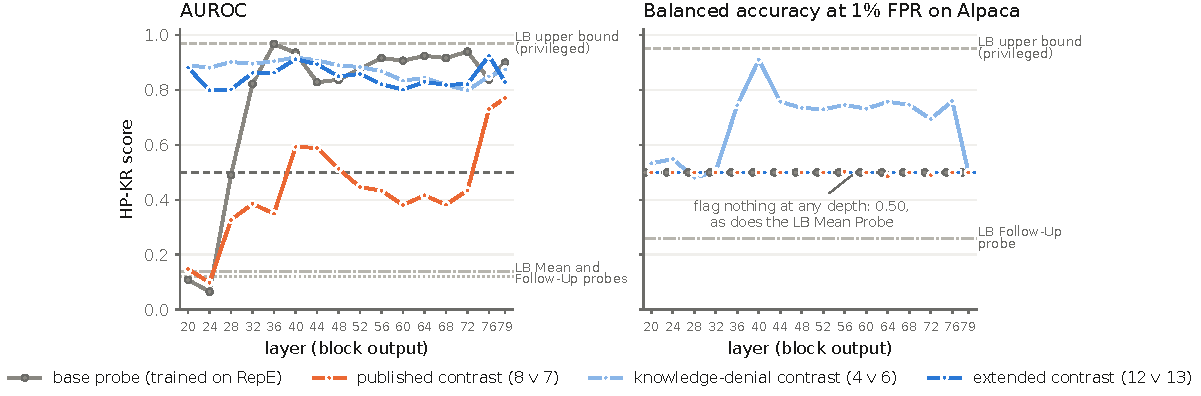
\includegraphics[width=\linewidth]{collab_fig_hpkr.pdf}
\caption{HP-KR AUROC and balanced accuracy of four detectors over 16 layers, as drawn by Pipeline~B.}
\label{fig:r-hpkr}
\end{figure}
% src: thesis/images/collab_fig_hpkr.pdf = git cat-file blob 16def2deec34aeee532511df116adb7de5522ca7:src/probes/deception-detection/paper/generated/fig_hpkr.pdf; git cat-file -s = 21,487 bytes = local file size; md5 f6757debe79d2951c6645abbc7a8f9c9 (both). Drawn by collaborator paper/make_figures.py @16def2de :: hpkr() from persona_ood_ext_L*/zero_shot.csv (AUROC) and zero_shot_operating.csv (balanced accuracy, threshold_source control); reference lines are Liars' Bench values transcribed in the collaborator's code (P.PAPER_PROBES).
% note: the figure's annotation "flag nothing at any depth: 0.50" is Pipeline B's wording; depth.csv puts the 8v7 arm at 0.4861-0.5026 (recall 0.0072 at L56 and L64), so the text gives the range.

\paragraph{How much of HP-KR is the words.}
The denial regular expression of Section~\ref{sec:m-integration}, which uses neither labels nor activations, reaches an AUROC of 0.9125 against HP-KR's label on all 2{,}139 rows. % src: recomputed 2026-09-25 from results/subsets/harm-pressure-knowledge-report.csv (model llama-v3.3-70b-instruct, n 2,139, 139 deceptive) with _DENIAL_RE / _ASSERT_RE of src/assistant_axis_ndif/eval_datasets.py :: 363-364, 385-388 :: roc_auc_score 0.9125432; chapter_5.tex :: 443
A trained raw probe does better, but not by much: on HP-KR's own held-out 20\%, at layer 40 with mean pooling, Pipeline~A's \texttt{raw} feature reaches an AUROC of 0.9741 with the \texttt{paper} probe, 0.9678 with \texttt{lr\_reg10} and 0.9623 with \texttt{mms}. % src: run-crossgen/kd11/matrices/mean_L40_s42.json :: results[feature=raw, probe=paper|lr_reg10|mms].auroc[2][2] (row = column = harm-pressure-knowledge-report); compared with 0.9125 above
Pipeline~B's raw-activation probe, scored on HP-KR by five-fold cross-validation with detection-token pooling, reaches 0.9458 at layer 40. % src: collaborator src/probes/deception-detection/results/persona_ood_ext_L40/matrix_baseline.csv @16def2de :: row = column harm_refusal_knowledge_report__plain (0.9458); diagonal by 5-fold stratified CV per deception_detection/scripts/persona_ood.py @16def2de :: 242-266
The response's length in tokens, with no training at all, ranks HP-KR's lies at an AUROC of 0.7756; the median lie is 7 tokens long and the median honest answer 5. % src: lab PC C:/Users/user4/expLB/run-coords/confounds_L44_last.json (cache audit/cache/labpc/run-coords/confounds_L44_last.json) :: confounds.length_only_auroc[dataset=harm-pressure-knowledge-report] :: auroc_from_length 0.7756115, median_pos 7.0, median_neg 5.0 (computed by 9_persona_probes.py :: 518-526 as roc_auc_score(label, span_len) on all rows)
Most of what separates HP-KR's classes is thus available from the text of the response, before any persona direction is read. % interp: regex 0.9125 and length 0.7756 against the raw probes' in-distribution 0.9623-0.9741 (Pipeline A, L40) and 0.9458 (Pipeline B, L40)

\paragraph{The factor probes.}
To separate the two things HP-KR's label mixes, we built two \emph{factor probes}: two directions, $d_{\text{knowledge}}$ and $d_{\text{utterance}}$, each of which probes one factor of the HP-KR label while the other is held fixed. % src: kd/scripts/build_factor_probes.py :: 1-27 (docstring); kd/docs/DESIGN.md :: 80-91
Both are built by teacher forcing on HP-KR's own items with the harm framing removed, so no response is generated. % src: kd/scripts/build_factor_probes.py :: 26-27 (no generation), 62-65 (harm preamble dropped, NEUTRAL_USER), 124 (prompt_fidelity "retemplated")
For $d_{\text{knowledge}}$, each of 1{,}962 items is forced to the same reply, ``I do not know the answer.'', and the classes are the 1{,}841 items the model knows and the 121 it does not. % src: kd/run/factor_probes/kd_knowledge/rows.jsonl (asix) :: 1,962 rows, response_str "I do not know the answer." on all, label {1: 1,841, 0: 121}; lab copy audit/cache/labpc/kd/run/factor_probes/kd_knowledge/rows.jsonl :: same label counts
For $d_{\text{utterance}}$, 900 known items each appear twice, once forced to that denial and once to ``I know the answer.''. % src: kd/run/factor_probes/kd_utterance/rows.jsonl (asix) :: 1,800 rows, label {1: 900, 0: 900}, response_str 900 x each; build_factor_probes.py :: 58-59 (DENY, ASSERT), 142-143 (--utterance_items 900)
Each direction is the difference of its two class means at each layer. % src: kd/scripts/phase2_gate.py :: 4-7 (docstring), 84-85 (diff_of_means)
Before using them we set a gate: $d_{\text{utterance}}$ should score near 1.0 on the knowledge-matched slice, where only the denial varies, and near 0.5 on the text-matched slice, where the wording is fixed; $d_{\text{knowledge}}$ should do the reverse. % src: kd/docs/DESIGN.md :: 93-95; kd/scripts/phase2_gate.py :: 11-19
On the knowledge-matched slice $d_{\text{utterance}}$ scores an AUROC of 0.9960, 0.9994 and 0.9995 at layers 20, 40 and 44 (post hoc). % src: lab PC C:/Users/user4/expLB/kd/results/phase2_gate.json (cache audit/cache/labpc/kd/results/phase2_gate.json, md5 1cdba3d2270a85fb6f9ec3b8e6652fee, MANIFEST.csv MATCH 2026-09-25) :: rows[layer 20/40/44].dU_knowledge_matched 0.9959971872126359 / 0.9994204421639917 / 0.9994745342286858; pooling mean; n_knowledge_matched 2001
On the text-matched slice, where the wording is fixed, it scores 0.3512 at layer 20 but 0.7842 and 0.7850 at layers 40 and 44. % src: same file :: rows[layer].dU_text_matched 0.3511675493500241 / 0.7841839191141069 / 0.7849662975445354; n_text_matched 258
$d_{\text{knowledge}}$ scores 0.6847, 0.7717 and 0.7706 on the text-matched slice and 0.3572, 0.6151 and 0.6597 on the knowledge-matched slice. % src: same file :: rows[layer].dK_text_matched 0.6847014925373134 / 0.7716658642272508 / 0.7705825710158883; dK_knowledge_matched 0.3571737668941109 / 0.6151001862312513 / 0.6597029572904513
So the gate passes at layer 20 and fails at layers 40 and 44, where the wording direction also separates the text-matched slice, on which the wording is the same in both classes. % interp: dU_text_matched 0.3512 at L20 against 0.7842 / 0.7850 at L40 / L44, against the gate's "near 0.5" criterion (kd/docs/DESIGN.md :: 93-95)
The two directions explain the failure: their cosine is 0.0630 at layer 20 but 0.4102 and 0.4304 at layers 40 and 44, so knowledge and wording are nearly orthogonal at layer 20 and entangled deeper in the network. % src: same file :: rows[layer].cos_dK_dU 0.0630229115486145 / 0.410187304019928 / 0.4303906261920929
$d_{\text{knowledge}}$ itself is stable: split halves of its 121-item minority class give directions with cosines 0.9876, 0.9955 and 0.9931, against a random-pair floor of 0.0079, 0.0089 and 0.0071. % src: same file :: rows[layer].split_half_cos 0.9876136183738708 / 0.995457649230957 / 0.9931256771087646; random_pair_cos 0.0079339355935195 / 0.008941260862981307 / 0.007102753421898463; class size: kd/run/factor_probes/kd_knowledge/rows.jsonl :: label 0 = 121
% note: the file holds only these three layers, one pooling (mean) and no bootstrap; the factor-probe activations behind it (kd/run/factor_probes/*/chunk_*.pt) are lab-only. The pre-committed reading of the gate (kd/docs/DESIGN.md :: 93-95) is stated above as it fell: pass at L20, fail at L40/L44 (ledger F-05, F-06).

\paragraph{The plain-assertion pole.}
Our two 4 v 3 contrasts split D8's honest pole into its sincere-ignorance and plain-assertion halves (Section~\ref{sec:m-banks}). % src: kd/personas/kd_role_groups.json :: contrasts knowledge_denial (neg sincere_ignorance), kd_assertion (neg plain_assertion)
Read zero-shot on full HP-KR in Pipeline~A, with the kd bank at scores 2--3 and mean pooling, the contrast of denial versus assertion (4 v 3) reaches an AUROC of 0.9118, 0.9344 and 0.9266 at layers 20, 40 and 44 (post hoc). % src: lab PC C:/Users/user4/expLB/run-crossgen/kd11/banks/collab/matrices/mean_L{20,40,44}_s42.json (cache audit/cache/labpc/run-crossgen/kd11/banks/collab/matrices/) :: zeroshot[direction=contrast:kd_assertion].auroc[harm-pressure-knowledge-report]
The knowledge denial contrast (4 v 3), whose two poles both deny, reaches only 0.5923, 0.6692 and 0.6659. % src: same files :: zeroshot[direction=contrast:knowledge_denial].auroc[harm-pressure-knowledge-report]
On the same bank, Pipeline~B's 4 v 6 contrast, which merges the two honest halves, reads 0.8734, 0.8826 and 0.8734 with detection-token pooling, between the two. % src: collaborator src/probes/deception-detection/results/persona_ood_mod_L{20,40,44}/zero_shot.csv @16def2de :: HP-KR row, auroc_denial_axis (0.8734137, 0.8825791, 0.8734173); bank as matched above by rollout counts (persona_ood_mod_L40/summary.md)
On the text-matched slice, where every response denies, the contrast of denial versus assertion falls to 0.4227, 0.5860 and 0.5253. % src: same collab cache files :: zeroshot[direction=contrast:kd_assertion].auroc[harm-pressure-kr-matched]
At layer 40, the one layer with a random-direction null for HP-KR under mean pooling, Pipeline~A's full-HP-KR readings in this subsection (0.9344, 0.8765 and 0.6692) all lie inside that null (Section~\ref{sec:r-stats}), so the evidence here is the fall from full HP-KR to the text-matched slice, not the height on full HP-KR. % src: run-coords/zeroshot_nulls.json :: corpus_L40_mean.per_dataset["harm-pressure-knowledge-report"].random_p95_auroc_dev 0.9377 (1,000 random directions, L40 mean; same rows as the kd11 grid: its deception_axis auroc 0.6436 = run-crossgen/kd11/matrices/mean_L40_s42.json zeroshot contrast on HP-KR); keys corpus_L40_mean and corpus_L44_last only (no L20, no L44 mean)
What these directions read on HP-KR is therefore mostly the difference between asserting and denying, not between a feigned and a sincere denial. % interp: denial v assertion 0.9118-0.9344 on full HP-KR, 0.4227-0.5860 on the text-matched slice; sincerity-only contrast 0.5923-0.6692 on full HP-KR; Pipeline B's merged 4v6 on the same bank 0.8734-0.8826
The trained features point the same way. % interp: next sentence's pairs
In Pipeline~A's train-one-test-all grid (11 datasets, mean pooling, \texttt{paper} probe, kd bank at score 3, $k=5$, one seed), \texttt{pc:kd\_assertion} averages 0.8119 off the diagonal at layer 40, against 0.7492 for \texttt{pc:knowledge\_denial}. % src: run-crossgen/kd11/banks/kd/matrices/mean_L40_s42.json :: results[feature=pc:kd_assertion|pc:knowledge_denial, probe=paper].auroc, mean of the 110 off-diagonal cells (0.8118620, 0.7491967); bank axes_vectors_s3.pt, k 5, seed 42
At layers 20 and 44 (post hoc) the pairs are 0.6389 against 0.6070 and 0.7926 against 0.7337. % src: run-crossgen/kd11/banks/kd/matrices/mean_L{20,44}_s42.json :: same fields (L20 0.6389122 / 0.6069568; L44 0.7926011 / 0.7337356)
Section~\ref{sec:r-transfer} sets \texttt{pc:kd\_assertion} against \texttt{raw} and the matched \texttt{datapca} control.

\paragraph{The convergence.}
Three tests remove the words of a denial as a cue, each in a different way, and Figure~\ref{fig:r-convergence} shows all three. % src: thesis_tools/figures/fig_convergence.py (stdout lists every plotted value)
We call their agreement \emph{the convergence}: where both classes deny knowledge, no persona direction reads the lie well, and where only the denial separates the classes, what separates them does not transfer. % interp: panels (a)-(c) below
We report it as one finding.

\emph{(a) The text-matched slice} (258 rows) fixes the wording: every response denies, and the label marks only whether the model knew (Section~\ref{sec:m-integration}). % src: chapter_5.tex :: 455 (258 rows; a lie is exactly "knows")
Pipeline~B never scored this slice, so Pipeline~A rebuilt its 12 v 13 grouping from the kd bank at scores 2--3; this is not the bank of Pipeline~B's main runs, which keeps score 3 only. % src: kd/personas/kd_role_groups_collab.json :: contrasts[name=collab_extended] (pos deception + knowledge_denial, neg honesty + sincere_ignorance + plain_assertion); cache json field bank "axes_collab_s23.pt"; Pipeline B datasets per chapter_5.tex :: 400 (no text-matched slice); git ls-tree -r 16def2de results/ has no matched-slice file
Zero-shot with mean pooling, the extended contrast reads the slice at an AUROC of 0.4630 [0.3970, 0.5400], 0.6203 [0.5535, 0.6845] and 0.5383 [0.4677, 0.6083] (row-bootstrap 95\% intervals) at layers 20, 40 and 44 (post hoc), against 0.8057, 0.8765 and 0.8491 on full HP-KR. % src: lab PC C:/Users/user4/expLB/run-crossgen/kd11/banks/collab/matrices/mean_L{20,40,44}_s42.json (cache audit/cache/labpc/run-crossgen/kd11/banks/collab/matrices/) :: zeroshot[direction=contrast:collab_extended].{auroc, ci95_lo, ci95_hi}[harm-pressure-kr-matched] and .auroc[harm-pressure-knowledge-report]
The knowledge denial contrast (4 v 3) reads 0.3932, 0.4989 and 0.4825, at or below 0.5 at all three layers. % src: same files :: zeroshot[direction=contrast:knowledge_denial].auroc[harm-pressure-kr-matched]
Over all twelve zero-shot directions of this bank (six contrasts and their first principal components), the slice reads 0.3932--0.5037 at layer 20, 0.4519--0.6887 at layer 40 and 0.4296--0.6211 at layer 44; the highest at layer 40 is the sycophancy contrast. % src: same files :: min/max over the 12 zeroshot directions, column harm-pressure-kr-matched (L20 knowledge_denial 0.3932 .. contrast 0.5037; L40 PC1:knowledge_denial 0.4519 .. contrast:sycophancy 0.6887; L44 PC1:knowledge_denial 0.4296 .. PC1:sycophancy 0.6211)
At layer 40, eight of the twelve directions have row-bootstrap intervals above 0.5, the extended contrast among them; so do five at layer 44 and none at layer 20. % src: same files :: count of zeroshot directions with ci95_lo[harm-pressure-kr-matched] > 0.5 -- L20 0/12; L40 8/12 (contrast, PC1, contrast:sycophancy, PC1:sycophancy, contrast:unified, PC1:unified, contrast:kd_assertion, contrast:collab_extended); L44 5/12 (contrast, PC1, contrast:sycophancy, PC1:sycophancy, contrast:unified)
A weak signal thus remains at the deeper layers, and at layer 40 it is strongest in the deception, sycophancy and unified directions (0.6409--0.6887), not the knowledge-denial ones; this panel has no random-direction null and no dataset bootstrap. % src: same files :: L40 kr-matched auroc contrast 0.6707, PC1 0.6628, contrast:sycophancy 0.6887, PC1:sycophancy 0.6846, contrast:unified 0.6859, PC1:unified 0.6409 (knowledge_denial 0.4989, kd_assertion 0.5860, collab_extended 0.6203); run-coords/zeroshot_nulls.json :: keys corpus_L40_mean, corpus_L44_last, sleeper_L44_last, sycophancy_mt (no harm-pressure-kr-matched entry)
% verified 2026-09-25: the draft said only that the extended contrast's interval lies above 0.5 at L40; 8 of 12 directions do.

\emph{(b) The knowledge-matched slice} (2{,}001 rows) fixes knowledge instead: the model knows every answer, so the label marks only the denial (Section~\ref{sec:m-integration}). % src: chapter_5.tex :: 455 (2,001 rows; a lie is exactly "denies")
Here the probe is trained on the slice's 80\% split, in a separate Pipeline~A run over 12 datasets with the leak guard on, the paper16 bank at score 3, mean pooling, the \texttt{paper} probe and seed 42. % src: lab PC C:/Users/user4/expLB-resplit/run-crossgen/km/matrices/mean_L{20,40,44}_s42.json (cache audit/cache/labpc/expLB-resplit/km/) :: fields datasets (12), design ("... AUDIT LEAK GUARD ..."), bank axes_vectors_s3_fp32.pt, bank_name paper16, pooling mean, seed 42
On the slice's own held-out 20\%, \texttt{raw} separates the classes almost perfectly: AUROC 0.9995, 0.9992 and 0.9993 at layers 20, 40 and 44 (post hoc). % src: same files :: results[feature=raw, probe=paper].auroc[i][i], i = harm-pressure-kr-knowledge-matched
Carried to the other 11 datasets, the four persona \texttt{axes} of Section~\ref{sec:m-features} transfer below chance at layers 20 and 40, at 0.3850 and 0.3335, and reach 0.5267 at layer 44. % src: same files :: results[feature=axes, probe=paper].auroc, mean of row i over the 11 other columns
\texttt{raw} transfers at 0.5711, 0.7093 and 0.7203, so \texttt{axes} $-$ \texttt{raw} is $-0.1860$, $-0.3758$ and $-0.1937$. % src: same files :: results[feature=raw, probe=paper] row-i off-diagonal mean; differences computed from the unrounded means
The persona axes also trail the matched \texttt{datapca} control (0.5208, 0.6636 and 0.7037) and a one-dimensional \texttt{length} feature (0.6174 at every layer). % src: same files :: results[feature=datapca|length, probe=paper] row-i off-diagonal mean
This run has one seed, one pooling and no dataset bootstrap. % src: same files :: seed 42, pooling mean; no significance file in audit/cache/labpc/expLB-resplit/km/
With knowledge fixed, the denial is easy to read inside its own dataset, and what the persona probe learns from it points the wrong way on most others. % interp: raw in-distribution 0.9992-0.9995 vs axes transfer 0.3850 / 0.3335 / 0.5267

\emph{(c) Gender-Secret} is Pipeline~B's test on the fine-tuned model of Liars' Bench that believes the user is male and denies knowing it, so both of its classes are denials. % src: log-only collaborator src/probes/deception-detection/results/gender_secret/summary.md @16def2de :: opening paragraph ("fine-tuned with a LoRA to believe the user is male and to deny knowing it. Both of its classes are denials")
Pipeline~B applied the adapter inside the remote pass and scored all 392 rows (116 lies) zero-shot, with the base model's persona directions from the kd bank at score 3 left unchanged and activations mean-pooled over the final answer. % src: same summary.md :: "How it was read" bullets (directions from "persona including knowlede denial/", not refitted; that folder is commit 148ddeb9); chapter_5.tex :: 596 (the 36 kd vectors on the Pipeline B branch are byte-identical to our vectors_s3); collaborator results/gender_secret/zero_shot.csv @16def2de :: n 392, n_deceptive 116
On this adapted read, the zero-shot AUROC of D8 is 0.5489, 0.4359 and 0.4979 at layers 20, 40 and 44 (post hoc), the extended contrast 0.5050, 0.4668 and 0.5409, the published contrast 0.5136, 0.5454 and 0.6231, and the sycophancy contrast 0.5927, 0.5230 and 0.5203. % src: collaborator src/probes/deception-detection/results/gender_secret/zero_shot.csv @16def2de :: rows read=adapted, detector {knowledge-denial (4v6), extended (12v13), published (8v7), sycophancy (5v5)}, column auroc (summary.md rounds these to 3 places)
At layer 40, where D8 reads HP-KR at 0.9185, its Gender-Secret interval is [0.3728, 0.4962], below 0.5. % src: zero_shot.csv :: layer 40, adapted, knowledge-denial (4v6) :: auroc_lo 0.3728, auroc_hi 0.4962; HP-KR 0.9185 from persona_ood_ext_L40/zero_shot_operating.csv
Of these twelve readings, two have intervals above 0.5: the sycophancy contrast at layer 20, 0.5927 [0.5303, 0.6555], and the published contrast at layer 44 (post hoc), 0.6231 [0.5647, 0.6757]. % src: zero_shot.csv :: adapted rows, auroc_lo > 0.5 only for (sycophancy (5v5), L20) and (published (8v7), L44)
Liars' Bench reports an AUROC of 0.45 for its Mean Probe and 0.24 for its Follow-Up Probe on this dataset and model \parencite[pp.~54--55]{kretschmar2025liars}. % src: kretschmar2025liars Table 6 p.54 and Table 7 p.55 :: Llama 3.3 70B row, GS column, AUROC
A probe trained on Gender-Secret itself separates the classes perfectly, but its lies are about gender and its honest answers about other attributes, so topic alone suffices. % src: log-only collaborator results/gender_secret/summary.md @16def2de :: "The information is there" bullet (5-fold CV AUROC 1.000 at every layer; topic alone suffices); no CSV holds the CV value
The lie was also instilled by fine-tuning, while the persona directions come from the base model's role-play, and Pipeline~B's summary names both differences as reasons the test is not conclusive on its own. % src: same summary.md :: "Two things keep this from being conclusive" (lie's source; topics)
Pipeline~A also scored Gender-Secret, through the base model with the paper16 bank and last-token pooling (Section~\ref{sec:r-organisms}); we use Pipeline~B's reading here because it applies the adapter and scores the kd contrasts. % src: src/assistant_axis_ndif/eval_datasets.py :: 262-267 (base model reads LoRA-generated rows), 283-284; run-coords/q11_sleeper_L{20,44}_last.json :: bank axes_vectors_s3_fp32.pt, pooling last, tests.zeroshot["gender-secret"]

The three tests differ in slice, pipeline, bank and protocol, and they agree. % interp: panels (a)-(c)
On the text-matched slice no zero-shot direction exceeds 0.6887 and the knowledge denial contrast stays at or below 0.5; on the knowledge-matched slice the trained persona axes transfer below chance at layers 20 and 40; on Gender-Secret no direction exceeds 0.6231 and D8 falls below 0.5 at layer 40. % interp: max over (a) 0.6887 (L40 sycophancy); (b) axes 0.3850 / 0.3335; (c) max 0.6231 (8v7, L44), 4v6 L40 0.4359 [0.3728, 0.4962]
On HP-KR, the persona directions' signal goes with the words of a denial, and where those words are controlled, none of the three tests finds more than a weak signal. % interp: the three panels together with the plain-assertion pole (0.9118-0.9344 full vs 0.4227-0.5860 text-matched)

\begin{figure}[t]
\centering
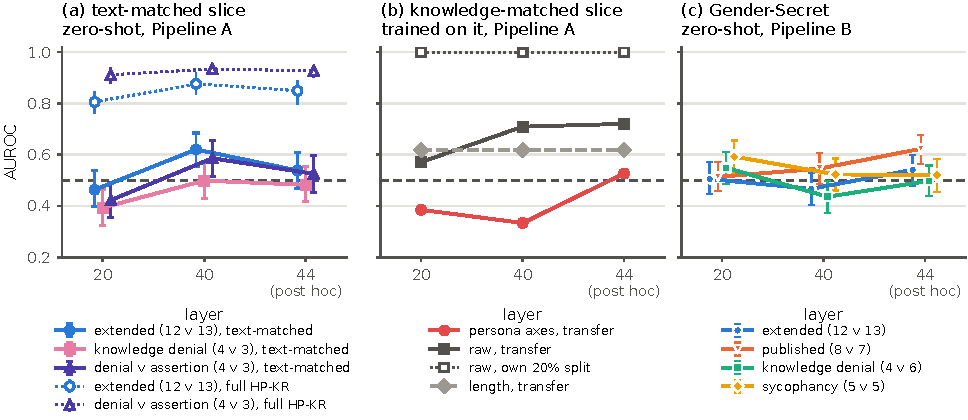
\includegraphics[width=\linewidth]{fig_convergence.pdf}
\caption{The convergence: three wording-controlled tests, AUROC by layer, with chance at 0.5.}
\label{fig:r-convergence}
\end{figure}
% src: thesis/images/fig_convergence.pdf, written by thesis_tools/figures/fig_convergence.py (run 2026-09-25; prints every plotted value; re-run by the verifier to a scratch path, output identical to the text). Panel (a): lab PC C:/Users/user4/expLB/run-crossgen/kd11/banks/collab/matrices/mean_L{20,40,44}_s42.json (cache audit/cache/labpc/run-crossgen/kd11/banks/collab/matrices/) :: zeroshot auroc, ci95_lo, ci95_hi. Panel (b): lab PC C:/Users/user4/expLB-resplit/run-crossgen/km/matrices/ (cache audit/cache/labpc/expLB-resplit/km/mean_L{20,40,44}_s42.json) :: results[axes|raw|length, paper]. Panel (c): collaborator src/probes/deception-detection/results/gender_secret/zero_shot.csv @16def2de :: read adapted, auroc, auroc_lo, auroc_hi.
% note: x positions are equally spaced (layers 20, 40, 44); L44 is labelled post hoc on the axis. Panel (a) error bars are row-bootstrap 95% intervals; panel (b) has none.

\paragraph{The trained test on the text-matched slice.}
Trained on the text-matched slice and tested on the other ten datasets, Pipeline~A's four paper16 \texttt{axes} score $-0.2545$, $+0.0309$ and $+0.0050$ above \texttt{raw} at layers 20, 40 and 44 (post hoc) once the leak guard is on (Section~\ref{sec:m-integration}; mean pooling, \texttt{paper} probe, seed 42), against $-0.2566$, $+0.0367$ and $+0.0134$ without it. % src: unguarded run-crossgen/kd11/matrices/mean_L{20,40,44}_s42.json :: same fields (axes - raw -0.2566 / +0.0367 / +0.0134); guarded lab PC C:/Users/user4/expLB-resplit/run-crossgen/matrices/mean_L{20,40,44}_s42.json (subfolder per audit/p17/fmap_F110_F127.csv; confirm on the lab PC) (cache audit/cache/labpc/expLB-resplit/mean_L{20,40,44}_s42.json) :: results[axes|raw, paper].auroc, row harm-pressure-kr-matched, mean over the 10 other columns (axes 0.3558 / 0.7468 / 0.7172; raw 0.6103 / 0.7159 / 0.7122); design "... AUDIT LEAK GUARD ..."; bank axes_vectors_s3_fp32.pt, bank_name paper16
The guard changes only the HP-KR cell of each of these averages. % verified 2026-09-25: row harm-pressure-kr-matched of results[axes|raw, paper] differs between the unguarded and guarded files only in column harm-pressure-knowledge-report, at L20, L40 and L44
In the other direction the guard matters more, and not always the same way: trained on full HP-KR, the persona axes rank the text-matched slice at 0.6004, 0.5674 and 0.6675 at layers 20, 40 and 44 with the leak, and at 0.7190, 0.4262 and 0.5667 without it, while \texttt{raw} moves from 0.6629, 0.7932 and 0.7930 to 0.5857, 0.7214 and 0.7214. % src: unguarded run-crossgen/kd11/matrices/mean_L{20,40,44}_s42.json and guarded cache audit/cache/labpc/expLB-resplit/mean_L{20,40,44}_s42.json :: results[axes|raw, paper].auroc[harm-pressure-knowledge-report][harm-pressure-kr-matched] (axes 0.6004454 / 0.5674049 / 0.6675494 -> 0.7190476 / 0.4261905 / 0.5666667; raw 0.6629153 / 0.7931512 / 0.7929706 -> 0.5857143 / 0.7214286 / 0.7214286)
Without the leak these cells rest on the 59 slice rows outside HP-KR's training split (Section~\ref{sec:m-integration}). % src: chapter_5.tex :: 460 (59 of 258); verified 2026-09-25: every guarded value x 630 is a half-integer, consistent with 59 rows split 14 / 45
The persona axes carry HP-KR to its own text-matched slice below chance only at layer 40; at layer 20 the guard raises them from 0.6004 to 0.7190. % interp: guarded 0.7190 / 0.4262 / 0.5667 vs leaked 0.6004 / 0.5674 / 0.6675
These guarded numbers have one seed and no dataset bootstrap. % src: guarded cache files above :: seed 42; only row_bootstrap_offdiag_* fields; no significance file in audit/cache/labpc/expLB-resplit/
% verified 2026-09-25: the draft reported the HP-KR -> text-matched cell at L40 only; L20 moves the other way.

On the store that samples 200 rows per dataset at all 80 layers (Section~\ref{sec:m-transform}), the same trained test, run with the kd bank at scores 2--3, gives \texttt{axes} 0.3743 at layer 20 and 0.7393 at layer 40, against \texttt{raw} 0.5904 and 0.7057 and \texttt{datapca} 0.6001 and 0.6738. % src: lab PC C:/Users/user4/expLB/run-crossgen/kd11/passA11/{banks/kd_s23/,}matrices/mean_L{20,40}_s42.json (cache audit/p17/labcache/expLB/run-crossgen/kd11/passA11/) :: results[axes (bank) | raw, datapca (root), paper].auroc, row harm-pressure-kr-matched, mean over the 10 other columns
This store's grid has no leak guard, so its HP-KR cell keeps the leak. % src: same files :: design "train on 80% of the row dataset; diagonal = its own 20% test split; off-diagonal = 100% of the column dataset" (no LEAK GUARD clause), all 160 matrices
At layer 40, fixed in advance, the margin of \texttt{axes} over \texttt{datapca} is $+0.0655$, with a 95\% interval of $[-0.0693, +0.1887]$ and $P(\text{margin} \le 0) = 0.1611$ when the 10 test datasets are resampled 10{,}000 times; it does not clear the dataset bootstrap. % src: computed 2026-09-25: python kd/scripts/layer_significance.py --bank audit/p17/labcache/expLB/run-crossgen/kd11/passA11/banks/kd_s23 --root audit/p17/labcache/expLB/run-crossgen/kd11/passA11 (B 10,000, seed 42, control datapca; 80 layers x 10 test datasets) :: "point +0.0655 95% CI [-0.0693, +0.1887] P(<=0) 0.1611"
Re-selecting the best layer inside each resample puts the peak anywhere from layer 5 to layer 79 (95\% interval), so the data cannot locate it. % src: same run :: "argmax layer ... 95% interval [L5, L79] width 74 layers of 80"
A cluster-based permutation test over 20 layers of the same store, with 200 label permutations and a random projection at the same $k$ as the control, gives $p=0.38$. % src: lab PC C:/Users/user4/expLB/run-premise/cluster_perm_kd_matched.json (cache audit/cache/labpc/run-premise/cluster_perm_kd_matched.json) :: p 0.38, B 200, layers (20: 0..76 step 4); control random at k=5 per src/assistant_axis_ndif/30c_cluster_perm.py :: 78, 101-120; run_dir run-coords/passA and bank run-kd/axes_vectors_s23.pt are the script defaults (:: 68, 80), not recorded in the JSON
The trained margin on the text-matched slice is therefore not significant at the pre-registered layer, inverts at layer 20, and has no locatable best layer. % interp: +0.0655 [-0.0693, +0.1887], P 0.1611; L20 axes 0.3743 below raw 0.5904 and datapca 0.6001; argmax interval L5-L79; cluster p 0.38

% ===== PART W4 (verified) =====
% ---------------------------------------------------------------------
% Part W4 (Chapter 5, file chapter_6.tex): sec:r-transfer, sec:r-personas, sec:r-selection.
% Every number was re-read from its raw file on 2026-09-25 with the script
% scratchpad w4/w4_numbers.py (session copy); its printed output is the verifier's reference.
% Collaborator files: git show 16def2de:src/probes/deception-detection/results/<path>.
% Independently re-verified 2026-09-25 (W4 verifier, scratchpad v4/*.py); fixes marked "% verifier:".
% ---------------------------------------------------------------------

\subsection{Transfer across datasets}
\label{sec:r-transfer}

Table~\ref{tab:r-transfer} shows how well each Pipeline~B arm transfers across Pipeline~B's six datasets. % src: collaborator src/probes/deception-detection/results/persona_ood_ext_L{20,40,44}/summary.csv @16def2de :: off_diagonal_mean, off_diagonal_excl_hpkr
Each entry is the mean AUROC over the 30 off-diagonal cells of the train-one-test-all matrix; the right half leaves HP-KR out as both source and test set, which keeps 20 cells. % src: collaborator paper/sections/setup.tex @16def2de :: 21-24; recomputed: off_diagonal_excl_hpkr = mean of the 20 cells with neither source nor target HP-KR (matrix_<arm>.csv, all arms, L20/40/44)
The persona arms use the kd bank at score 3, every arm reads the mean over the detection tokens, and the run has one seed (42) and no bootstrap of these means. % src: collaborator paper/sections/method.tex @16def2de :: 61 (keep only responses scored 3), 121 (mean-pool the detection tokens); results/persona_ood_ext_L20/summary.md @16def2de :: 3 (persona including knowlede denial/, 36 personas); deception_detection/scripts/persona_ood.py @16def2de :: 62 (SEED = 42); summary.csv has no interval columns (features, layer, dim, off_diagonal_mean, off_diagonal_excl_hpkr, diagonal_mean)
Layers 20 and 40 were fixed in advance, and layer 44 is post hoc (Section~\ref{sec:m-layers}). % src: git show 63aabb4b:docs/LAYER_PREREGISTRATION.md :: 20-26 (L20 and L40 independent of our outcome; L44 "our own sweep ... NO")

\begin{table}[t]
\centering
\footnotesize
\caption{Transfer: mean off-diagonal AUROC of Pipeline~B's arms on its six datasets (layer 44 post hoc).}
\label{tab:r-transfer}
\begin{tabular}{p{50mm}rcccccc}
\hline
 & & \multicolumn{3}{c}{All six test sets} & \multicolumn{3}{c}{Excluding HP-KR} \\
Arm & Dim. & L20 & L40 & L44 & L20 & L40 & L44 \\
\hline
Raw probe (D1) & 8192 & 0.648 & 0.732 & 0.716 & 0.728 & 0.758 & 0.730 \\
\hline
Published contrast, 8 v 7 (D5) & 1 & 0.651$^{a}$ & 0.832 & 0.826 & \textbf{0.919} & 0.880 & 0.873 \\
Knowledge-denial contrast, 4 v 6 (D8) & 1 & 0.866 & 0.912 & 0.900 & 0.861 & 0.910 & 0.899 \\
Extended contrast, 12 v 13 (D9) & 1 & \textbf{0.904} & \textbf{0.916} & \textbf{0.903} & 0.909 & \textbf{0.917} & \textbf{0.905} \\
\hline
Extended PCs, $k=3$ (D4, kd bank) & 3 & 0.684 & 0.866 & 0.880 & 0.900 & 0.867 & 0.870 \\
Extended PC1 & 1 & 0.661 & 0.768 & 0.780 & 0.682 & 0.774 & 0.793 \\
Published PCs, $k=3$ (D4) & 3 & 0.679 & 0.639 & 0.617 & 0.888 & 0.751 & 0.728 \\
Random directions, $k=3$ & 3 & 0.527 & 0.504 & 0.493 & 0.560 & 0.544 & 0.547 \\
\hline
\multicolumn{8}{p{140mm}}{$^{a}$ A sign artifact (see the text); with the sign restored, 0.7909; best value per column in bold.} \\
\end{tabular}
\end{table}
% src: collaborator results/persona_ood_ext_L{20,40,44}/summary.csv @16def2de :: rows baseline, axis1, denial_axis1, ext_axis1, ext_pc3, ext_pc1, pc3, random3; columns off_diagonal_mean, off_diagonal_excl_hpkr; rounded to 3 dp (full values printed by w4_numbers.py section A)
% verified: identical, cell for cell, to collaborator paper/generated/tab_transfer.tex @16def2de (make_numbers.py output)
% src: footnote 0.7909 -- collaborator results/persona_ood_ext_L20/matrix_axis1.csv @16def2de, HP-KR source row with 1 - AUROC in its five off-diagonal cells, off-diagonal mean = 0.7909 = mean of zero_shot.csv :: auroc_axis over the six datasets
% verifier: "best value per column" is over the arms shown; summary.csv arms not in the table (pc1, syc_pc1, syc_axis1, uni_axis1) reach 0.916-0.937 excluding HP-KR

A one-dimensional arm can learn only a sign, so its off-diagonal mean equals its zero-shot mean over the six datasets whenever every source agrees on that sign (Section~\ref{sec:m-protocols}). % src: collaborator paper/sections/setup.tex @16def2de :: 24-26
At layers 40 and 44 the two agree to four decimals for the four one-dimensional arms of Table~\ref{tab:r-transfer}; the extended contrast, for example, reads 0.9158 both ways at layer 40. % src: collaborator results/persona_ood_ext_L{40,44}/summary.csv :: off_diagonal_mean (axis1 0.8319/0.8260, denial_axis1 0.9115/0.9001, ext_axis1 0.9158/0.9034, ext_pc1 0.7680/0.7801) = mean of zero_shot.csv :: auroc_axis, auroc_denial_axis, auroc_ext_axis, auroc_ext_pc1 over the six labelled rows (same values)
Among these arms, the published contrast at layer 20 is the exception. % src: persona_ood_ext_L20/summary.csv :: axis1 off_diagonal_mean 0.6511 vs zero_shot.csv mean auroc_axis 0.7909
% verifier: outside the table the same artifact hits syc_axis1 and syc_pc1 (L20, L40), syc_axis1 (L44), pc1 (L20) and uni_axis1 (L20 0.6295 vs 0.7653; L40 0.6897 vs 0.8295) -- uni_axis1 is missing from F-124 section 1's "seven cells"
We call this a \emph{sign artifact}: a trained one-dimensional probe inherits a reversed sign from its training set, so its score on every other test set is one minus the zero-shot AUROC. % note: new term, defined here (glossary addition); mechanism per collaborator setup.tex @16def2de :: 24-28
At layer 20 the published contrast ranks HP-KR in reverse (Section~\ref{sec:r-problem}), so the probe trained on HP-KR learns the opposite sign and scores the other five datasets between 0.0065 and 0.2831. % src: collaborator results/persona_ood_ext_L20/matrix_axis1.csv @16def2de :: row harm_refusal_knowledge_report__plain (CG 0.0601, HP-C 0.2831, IT 0.0121, ID 0.0413, RepE 0.0065)
With that row's sign restored, the off-diagonal mean is 0.7909, which is the contrast's zero-shot mean; the table's 0.651 reflects the training set, not the direction. % src: computed from matrix_axis1.csv L20 (w4_numbers.py section B) :: 0.7909; zero_shot.csv L20 :: mean auroc_axis 0.7909

Over all six datasets, the extended contrast (D9) transfers best at all three layers, at 0.904, 0.916 and 0.903. % src: summary.csv L20/40/44 :: ext_axis1 off_diagonal_mean 0.9041, 0.9158, 0.9034
The raw probe trails it by 0.256, 0.184 and 0.188, and random directions ($k=3$, averaged over five draws) stay between 0.493 and 0.527. % src: summary.csv :: ext_axis1 - baseline off_diagonal_mean (0.9041-0.6478, 0.9158-0.7320, 0.9034-0.7156); random3 0.5269, 0.5038, 0.4927; five draws: collaborator method.tex @16def2de :: 112, persona_ood.py @16def2de :: 61 (N_RANDOM_DRAWS = 5)
Pipeline~B has no dataset-PCA or length control; Pipeline~A's controls are given below. % src: summary.csv @16def2de :: features column (baseline, pc1, pc3, axis1, random3, syc_*, dec3_orth, ext_*, denial_*, uni_*; no datapca, no length)
Much of D9's lead over the published contrast comes from HP-KR. % interp: D9 - D5 at L40 is 0.084 over all six and 0.037 excluding HP-KR; at L20 D5 leads excluding HP-KR
At layer 40 the lead is 0.084 over all six datasets and 0.037 without HP-KR. % src: summary.csv L40 :: ext_axis1 - axis1, off_diagonal_mean 0.9158-0.8319; off_diagonal_excl_hpkr 0.9165-0.8798
At layer 20, without HP-KR, the published contrast leads, at 0.919 against 0.909. % src: summary.csv L20 :: off_diagonal_excl_hpkr axis1 0.9194, ext_axis1 0.9086
Section~\ref{sec:r-d4} discusses the principal-component arms.

Over Pipeline~B's 16-layer sweep, the extended contrast leads the single-source raw probe at every layer, by 0.115 (layer 60) to 0.273 (layer 24). % src: collaborator results/persona_depth/depth.csv @16def2de :: source "transfer, off-diagonal mean", metric auroc, extended axis (12v13) - single-source probe (8192-d): min +0.1150 at L60, max +0.2731 at L24, positive 16/16
It is the best of the sweep's six arms at 12 of the 16 layers; the knowledge-denial contrast leads at layer 28 and the extended PCs at layers 64--72. % src: depth.csv :: same source and metric, arg-max arm per layer: extended axis (12v13) at L20, 24, 32, 36, 40, 44, 48, 52, 56, 60, 76, 79; knowledge-denial axis (4v6) at L28; extended PCs (k=3) at L64, 68, 72
% verifier: depth.csv's 8v7 and 13v12 transfer rows carry the sign artifact at 12 and 13 of 16 layers; with the sign restored neither reaches the extended contrast at any layer, so the arg-max count is unchanged. D9 and D8 equal their zero-shot means at all 16 layers.
Its best transfer is 0.9275 at layer 36, against 0.9158 at layer 40; the raw probe reads 0.7682 and 0.7320 at those two layers. % src: depth.csv :: extended axis (12v13) L36 0.9274688514303678, L40 0.9158352734669752; single-source probe (8192-d) L36 0.7682162964601599, L40 0.7320069613011962
Layer 36 is post hoc, and 13 of the 16 layers, layer 36 among them, were pooled by code that is not in the repository (Section~\ref{sec:m-transform}). % src: git show -s ea1ce52b (subject: "ranking peaks at 36", after L40 was fixed); collaborator deception_detection/scripts/layer_sweep.py @16def2de :: 39 (NEW_LAYERS = 24, 28, 32, 36, 48-79: 13 layers); Chapter 4 sec:m-transform disclosure
Section~\ref{sec:r-layer} discusses the depth profile.

Figure~\ref{fig:r-transfer} shows the two matrices behind D1 and D9 at layer 40. % src: collaborator paper/make_figures.py @16def2de :: 60-90 (transfer_matrices(layer=40): panels matrix_baseline.csv and matrix_ext_axis1.csv)
In the left panel the raw probe fits each training set but transfers unevenly, and several cells fall below chance; the probe trained on RepE, for instance, scores IT at 0.2735 (Section~\ref{sec:r-supervised}). % src: collaborator results/persona_ood_ext_L40/matrix_baseline.csv @16def2de :: diagonal 0.9458-1.0; row repe_honesty__plain, column insider_trading_cadenza__plain = 0.2735; 6 of 30 off-diagonal cells below 0.5
Off the diagonal, the right panel is constant along each test row by construction. % src: collaborator results/persona_ood_ext_L40/matrix_ext_axis1.csv @16def2de :: every off-diagonal cell of a test column within 0.0002 of the others (e.g. HP-C 0.7115-0.7116, IT 0.9801-0.9803); the five-fold diagonal cells differ by at most 0.001 (CG 0.9113 vs 0.9123), equal at the figure's two decimals
A probe on one feature learns only a sign, and all six training sets agree on it at layer 40, so each row repeats the test set's zero-shot AUROC. % src: setup.tex @16def2de :: 24-26; zero_shot.csv L40 :: auroc_ext_axis
The panel therefore shows the zero-shot scores, not a transfer effect. % interp: follows from the constant rows (matrix_ext_axis1.csv L40) and the one-feature argument (setup.tex :: 24-26)

\begin{figure}[t]
\centering
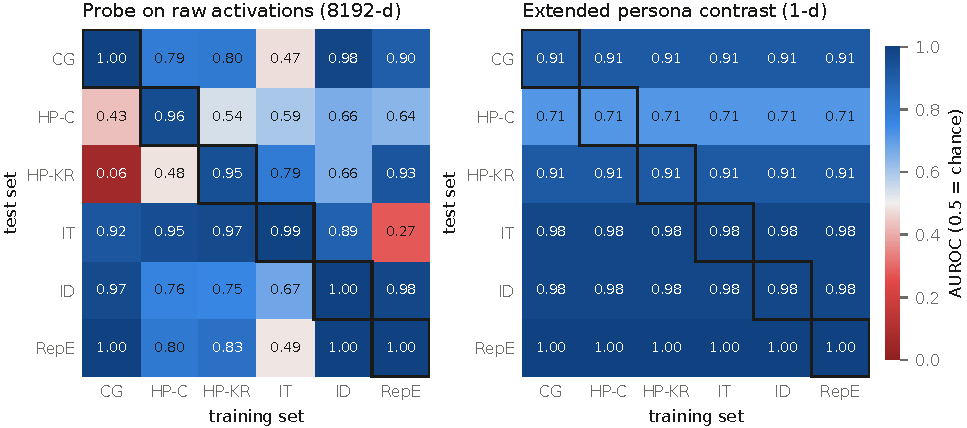
\includegraphics[width=\linewidth]{collab_fig_transfer.pdf}
\caption{Train-one-test-all AUROC at layer 40 for D1 (left) and D9 (right); produced by Pipeline~B.}
\label{fig:r-transfer}
\end{figure}
% src: thesis/images/collab_fig_transfer.pdf = git cat-file blob 16def2deec34aeee532511df116adb7de5522ca7:src/probes/deception-detection/paper/generated/fig_transfer.pdf (blob 4407f9fbbf4b19078cc3f04e14df0cc298878349; git cat-file -s = 17,357 bytes = file size; md5 0c78dc1c3f3be7c574fae4a402e91e16); rows = test set, columns = training set, boxed diagonal in-distribution

Pipeline~A scores the same contrast on its eleven datasets. % src: kd/personas/kd_role_groups_collab.json :: 61-71 (collab_extended = deception + knowledge_denial v honesty + sincere_ignorance + plain_assertion, 12 v 13)
For this run we rebuilt the 12 v 13 grouping on the kd bank at scores 2--3, not at score 3. % src: lab PC C:/Users/user4/expLB/run-crossgen/kd11/banks/collab/matrices/mean_L40_s42.json (cache audit/cache/labpc/run-crossgen/kd11/banks/collab/matrices/mean_L40_s42.json) :: bank "axes_collab_s23.pt"
Zero-shot, its mean AUROC over the eleven datasets is 0.7996 at layer 40, against 0.7325 for the published contrast built from the same bank. % src: lab PC C:/Users/user4/expLB/run-crossgen/kd11/banks/collab/matrices/mean_L40_s42.json (cache audit/cache/labpc/run-crossgen/kd11/banks/collab/matrices/mean_L40_s42.json) :: zeroshot[direction=contrast:collab_extended].auroc mean over 11 = 0.7996; zeroshot[direction=contrast].auroc mean = 0.7325
At layer 20 it reads 0.7386, and at layer 44 (post hoc) 0.7745. % src: lab PC .../kd11/banks/collab/matrices/mean_L{20,44}_s42.json (cache audit/cache/labpc/run-crossgen/kd11/banks/collab/matrices/) :: zeroshot[contrast:collab_extended].auroc mean over 11
For reference, Pipeline~A's trained controls at layer 40 average 0.6623 for the raw probe, 0.6651 for \texttt{datapca@5} and 0.5849 for \texttt{random@5}, over the 110 off-diagonal cells (mean pooling, \texttt{paper} probe, 80/20 split, seed 42). % src: run-crossgen/kd11/matrices/mean_L40_s42.json (asix; md5 d7616aa5... identical to the lab-PC cache) :: results[feature=raw|datapca|random, probe=paper].auroc, mean of the 110 off-diagonal cells
These controls are trained probes, whereas the contrast is zero-shot, and we did not run the random-direction null for this contrast; Section~\ref{sec:r-stats} gives the response-length control. % src: no zero-shot null for contrast:collab_extended in run-coords/*.json (grep, 2026-09-25); run-coords/zeroshot_nulls.json covers the paper16 bank only (25_zeroshot_nulls.py :: 80, --bank run-paper16/axes_vectors_s3_fp32.pt)
The gap between 0.7996 here and Pipeline~B's 0.9158 comes from the dataset sets, not from the pipelines. % interp: on the five shared datasets the two agree to 0.011 (next line), and bank-matched cells agree to 0.0015 (below)
On the five Liars' Bench datasets both pipelines score, our rebuild reads 0.8882, which is 0.011 below Pipeline~B's average for the same contrast (Section~\ref{sec:r-zeroshot}); the published contrast reads 0.7868 in our pipeline and 0.7983 in Pipeline~B. % src: cache audit/cache/labpc/run-crossgen/kd11/banks/collab/matrices/mean_L40_s42.json :: zeroshot mean over ID, HP-C, HP-KR, CG, IT = 0.8882 (collab_extended), 0.7868 (contrast); collaborator results/persona_ood_ext_L40/zero_shot.csv @16def2de :: mean over the same five = 0.8990 (auroc_ext_axis), 0.7983 (auroc_axis); 0.8990 - 0.8882 = 0.0108
The remaining gap is the judge filter of the bank, score 3 against scores 2--3. % interp: bank-matched cells agree to a mean |gap| of 0.0015 (next paragraph), so the 0.011 is the bank, not the pipeline; also Pipeline B's own scores 2-3 re-extraction, collaborator results/persona_ood_mod_L40/zero_shot.csv @16def2de, reads 0.8879 (auroc_ext_axis) and 0.7859 (auroc_axis) on the same five

A trained feature built on the kd bank shows how far a persona basis gets against the matched control. % src: lab PC C:/Users/user4/expLB/run-crossgen/kd11/banks/kd/significance.json (cache audit/cache/labpc/run-crossgen/kd11/banks/kd/significance.json, md5 af3b9feb807722c23afb6e35fc4629eb, 6,300 tests)
\texttt{pc:kd\_assertion} is the top five principal components of the kd bank at score 3, taken over the four knowledge-denial roles, the three plain-assertion roles and the anchor (Section~\ref{sec:m-features}); Section~\ref{sec:r-hpkr} gives its off-diagonal AUROC. % src: src/assistant_axis_ndif/6_axes.py :: 247-249, 260-267 (a declared contrast gets its own PCA basis over the roles it contrasts plus the anchor); kd/personas/kd_role_groups.json :: contrasts[kd_assertion] (knowledge_denial v plain_assertion, no basis key); 27_crossgen.py :: 882 (k = 5)
At layer 40, on the eleven datasets with mean pooling and the \texttt{paper} probe, it beats the raw probe by $+0.150$ (dataset-bootstrap interval $[+0.070, +0.237]$) and the matched \texttt{datapca@5} control by $+0.147$ ($[+0.059, +0.258]$). % src: cache audit/cache/labpc/run-crossgen/kd11/banks/kd/significance.json :: tests[block=10, pooling=mean, probe=paper, layer=40, comparison="pc:kd_assertion - raw"] diff 0.149588, dataset_ci95 [0.070245, 0.236626]; comparison "pc:kd_assertion - datapca" diff 0.146779, dataset_ci95 [0.058764, 0.258211]
Both intervals exclude zero, but neither difference survives the Benjamini--Hochberg correction, which runs over every pooling, layer, probe and comparison in the block ($q=0.073$ for both). % src: same file :: note ("BH within each block over every pooling x layer x probe x comparison"); dataset_q_bh 0.073256 (both); significant_datasets False (both)
Across the 21 layers it beats the raw probe at 18 and clears the correction at one, layer 68. % src: same file :: block 10, mean, paper, "pc:kd_assertion - raw": diff > 0 at 18/21 layers (negative at L0, L12, L16); significant_datasets True only at L68 (q 0.0467)
Against \texttt{datapca} it is ahead at 20 of 21 layers, and none of the 126 tests (21 layers, two poolings, three probes) clears. % src: same file :: "pc:kd_assertion - datapca", block 10 (all 11 datasets): diff > 0 at 20/21 layers (mean, paper; negative at L16); 126 tests, 0 with significant_datasets True
% interp: the kd bank's register basis is ahead of the matched control almost everywhere, but no single test of that lead is significant at the dataset level
% note: kd11 "block 10" = all eleven datasets (27_crossgen.py :: 781, block "10" = range(n)); "block 9" = ten, without sycophancy_mt (kd11 matrix JSON :: block9 list)

The two pipelines agree when they score the same persona bank on the same rows: over 50 bank-matched zero-shot cells, the mean absolute gap is 0.0015 and the largest is 0.0175 (Appendix~\ref{app:repro}). % src: computed 2026-09-25 (w4_numbers.py section G; re-run by the verifier, v4/vG.py, same result): collaborator results/persona_ood_{ext,mod}_L{20,40,44}/zero_shot.csv and persona_ood_L40/zero_shot.csv @16def2de :: auroc_axis, auroc_ext_axis, against run-crossgen/kd11/banks/kd/matrices/mean_L{20,40,44}_s42.json (asix; kd score 3, 8 v 7: 15 cells, 0.0015), cache audit/cache/labpc/run-crossgen/kd11/banks/collab/matrices/mean_L{20,40,44}_s42.json (kd scores 2-3, 8 v 7: 15 cells, 0.0017; 12 v 13: 15 cells, 0.0015), run-crossgen/banks/paper16_shared/matrices/mean_L40_s42.json (asix; 8 v 7 at L40: 5 cells, 0.0012); five datasets ID, HP-C, HP-KR, CG, IT
% note: audit/phase3/DISAGREEMENTS.md section 0 reports 55 cells; the other 5 (paper16_shared at L20) need a lab-PC matrix with no local copy and were not re-read.
% note: the two pipelines' raw baselines differ in protocol (audit D-04), so their margins over raw are never compared in one sentence.

% ---------------------------------------------------------------------
\subsection{Which personas: library and purpose-built banks}
\label{sec:r-personas}

Section~\ref{sec:m-banks} describes two kinds of bank.
The purpose-built banks, paper16 and kd, have roles written for one behaviour each; the library banks, own100 and hf275, take their roles from the Assistant-Axis library. % src: tab:m-banks; src/assistant_axis_ndif/role_groups.json (own100); run-hf275/vectors_275 (hf275)
This section asks whether the kind of bank matters.
Two reference directions are needed. % src: src/assistant_axis_ndif/6_axes.py :: 156-165
A bank's own \emph{assistant direction} is the mean vector of its assistant anchor minus the mean over all its other roles. % src: src/assistant_axis_ndif/6_axes.py :: 157-165 (assistant_axis = mean(default_like) - mean(role_side))
The \emph{published Assistant Axis} is the axis released by \textcite[p.~6]{lu2026assistant}, built the same way from their role vectors; we use the released Llama-3.3-70B file. % src: lu2026assistant PDF p.6 ("We subtracted the mean of all fully role-playing role vectors from the mean default Assistant activation ... at every layer"); src/assistant_axis_ndif/31_fetch_hf_vectors.py :: 21, 33-35 (lu-christina/assistant-axis-vectors, llama-3.3-70b/assistant_axis.pt); run-hf275/published_assistant_axis.pt (owner laptop, untracked) md5 2807d7caa7f5f0126be9ba4c4b6ea906 = the HF cache copy
The published axis is one fixed reference for every bank, whereas a bank's own direction depends on that bank's roles. % interp: by construction (6_axes.py :: 156-165)
The two can differ a great deal: paper16's own direction has a cosine of only 0.2997 to 0.3719 with the published axis at layers 20, 22, 40 and 60. % src: run-paper16/axes_vectors_s3.pt (owner laptop, untracked; md5 5d05a42542ae13fc7ac5d893a4ae4f8c) :: axes.assistant[L] vs run-hf275/published_assistant_axis.pt[L]: L20 0.3662, L22 0.3059, L40 0.3719, L60 0.2997
For hf275 they coincide: the direction rebuilt from the 275 released role vectors has a cosine of at least 0.9999 with the released axis at those layers. % src: run-hf275/vectors_275/*.pt (276 files: 275 roles + default) :: default - mean(other 275) vs published axis: L20 0.99995, L22 0.99990, L40 0.99997, L60 0.99994

\begin{table}[t]
\centering
\footnotesize
\caption{Cosine of each bank's deception contrast with an assistant direction, by layer.}
\label{tab:r-personas}
\begin{tabular}{lcccccc}
\hline
 & \multicolumn{4}{c}{Against the bank's own assistant direction} & \multicolumn{2}{c}{Against the published axis} \\
Layer & paper16 & own100$^{a}$ & hf275$^{b}$ & kd, 12 v 13 & paper16 & kd, 12 v 13 \\
\hline
L20 & $-0.364$ & $-0.729$ & $-0.686$ & $-0.394$ & $-0.168$ & $-0.246$ \\
L22 & $-0.338$ & $-0.710$ & $-0.662$ & $-0.372$ & $-0.141$ & $-0.223$ \\
L40 & $-0.370$ & $-0.660$ & $-0.610$ & $-0.374$ & $-0.226$ & $-0.264$ \\
L60 & $-0.374$ & $-0.573$ & $-0.516$ & $-0.366$ & $-0.180$ & $-0.230$ \\
\hline
\multicolumn{7}{p{140mm}}{$^{a}$ Provisional: a log-only diagnostic of 2026-09-14, not re-read. $^{b}$ own100's 22 v 22 grouping on Lu et al.'s released vectors, measured against the published axis, which is this bank's own direction to a cosine of at least 0.9999. paper16 (8 v 7) and kd are at score 3.} \\
\end{tabular}
\end{table}
% src: paper16 -- run-paper16/axes_vectors_s3.pt (owner laptop, untracked; md5 5d05a42542ae13fc7ac5d893a4ae4f8c) :: cos(axes.deception[L], axes.assistant[L]) = -0.364137, -0.337642, -0.370490, -0.374159; vs published: -0.167654, -0.140737, -0.226271, -0.179980
% src: own100 -- lab PC C:/Users/user4/expLB/run/axes.pt (no local cache; not re-read); values as printed by the 2026-09-14 diagnostics and tabulated in docs/thesis/persona-coordinates-70b-results.md :: section 7.1 (table lines 523-528), a map, not a source -- PROVISIONAL, re-read on the lab PC
% src: hf275 -- run-hf275/vectors_275/*.pt :: mean(22 deception roles) - mean(22 honesty roles), groups from run-hf275/axes_hf100.pt :: role_groups (= src/assistant_axis_ndif/role_groups.json deception/honesty), against run-hf275/published_assistant_axis.pt: -0.6856, -0.6621, -0.6097, -0.5161 (against the rebuilt 275-role direction: -0.6854, -0.6614, -0.6088, -0.5180)
% src: kd -- audit/p17/labcache/expLB/run-kd/vectors_s3/*.pt (36 files, md5-identical to the lab PC and to collaborator commit 148ddeb9) with kd/personas/kd_role_groups.json :: groups; 12 v 13 = deception + knowledge_denial v honesty + sincere_ignorance + plain_assertion; own direction = default - mean(35 others): -0.393742, -0.371884, -0.374031, -0.365673; vs published: -0.245549, -0.223322, -0.263838, -0.229794
% verified: audit/scripts/claims/W6A_geom.py gives the same paper16, hf275 and paper16-vs-published columns; the W4 verifier recomputed every non-own100 cell from the same files (v4/vH.py, vH2.py, vK.py).

Table~\ref{tab:r-personas} shows that the library banks' deception contrasts point strongly away from the assistant direction: at layer 40 their cosine with it is $-0.660$ for own100 and $-0.610$ for hf275. % src: table above (own100 log-only; hf275 recomputed)
paper16's deception contrast reads $-0.370$ against its own direction and $-0.226$ against the published axis, and the kd bank's extended contrast (D9) reads $-0.374$ and $-0.264$. % src: table above
Against the one shared reference, the purpose-built contrasts at layer 40 therefore have less than half the library contrast's cosine in magnitude. % interp: -0.226 and -0.264 against -0.610 (published axis, L40)
paper16's contrast stays between $-0.248$ and $-0.115$ against the published axis at every layer from 20 to 60. % src: run-paper16/axes_vectors_s3.pt vs published axis, all 41 layers L20..L60 :: min -0.2481, max -0.1146
The own100 column is provisional: that bank's vectors are only on the lab machine, and we have not re-read them; its values come from a diagnostic run of 2026-09-14. % src: docs/thesis/persona-coordinates-70b-results.md :: 535-536 ("The own100 column comes from the 2026-09-14 diagnostics. The own100 bank is on the lab PC and was not re-read."); no local copy of lab PC C:/Users/user4/expLB/run/axes.pt
% verifier: the writer's "saved no result file" is not established -- the bank file itself (run/axes.pt) is on the lab PC and would reproduce the column; only the diagnostic's printout is unsaved.

Over all the roles of a library bank, the leading principal component lies close to the assistant direction. % interp: the PC1 cosines in the next two lines
Over own100's 100 roles, taken from Lu et al.'s released vectors, PC1 has an absolute cosine of 0.7544 to 0.8025 with the published axis at layers 20, 22, 40 and 60. % src: run-hf275/axes_hf100.pt (owner laptop, untracked; md5 02a548364325ba769679265f6c4dc04c; vectors_dir run-hf275/vectors_100) :: pca.all.components[L,0] (100 roles) vs published axis: 0.8025, 0.7938, 0.7814, 0.7544
The 2026-09-14 diagnostic gave 0.73 to 0.82 on own100's own vectors against their own direction (provisional). % src: log-only diagnostics 2026-09-14 (lab PC run/axes.pt, not re-read), as recorded in docs/thesis/persona-coordinates-70b-results.md :: 545-546 (a map)
\textcite[p.~6]{lu2026assistant} report the same for their full role set: the similarity between PC1 and the Assistant Axis is above 0.60 at all layers and above 0.71 at the middle layer. % src: lu2026assistant PDF p.6, Section 3.1 (">0.60 at all layers across our three models, and >0.71 at the middle layer of each model (Appendix G.1)")
PCA over a whole role library therefore recovers assistant-likeness first, whatever behaviour the roles were grouped for. % interp: PC1 |cos| 0.75-0.80 with the published axis (above) and Lu et al. p.6; applies to the all-roles basis, not to a per-behaviour basis
The purpose-built paper16 bank behaves differently: its PC1 over all 26 roles has an absolute cosine of only 0.0089 to 0.1186 with the published axis. % src: run-paper16/axes_vectors_s3.pt :: pca.all.components[L,0] vs published axis: L20 0.1186, L22 0.0724, L40 0.0898, L60 0.0089
It is, however, close to paper16's own assistant direction, at 0.7891 to 0.8187. % src: same file :: |cos(pca.all.components[L,0], axes.assistant[L])| = 0.8145, 0.8187, 0.8162, 0.7891
That own direction is not a clean reference: paper16's anchor answered only the deception questions, so the direction also separates paper16's two question sets, with a cosine of 0.767 at layer 40 with the direction between them. % src: run-paper16/responses/default.jsonl :: question_index 0-9 only (the 10 deception questions); computed from run-paper16/vectors_s3/*.pt and axes_vectors_s3.pt: cos(axes.assistant[40], mean(15 deception/honesty roles) - mean(10 sycophancy/anti-sycophancy roles)) = 0.7672 (anchor left out of both means)
% interp: paper16's all-roles PC1 uses the same 26 roles as its unified basis, which tracks the question set (cos -0.980, below); its own assistant direction shares that component

Relabelling the library does not remove the alignment. % interp: 10.6% reduction (next lines)
We regrouped the released role vectors by the stance of each role toward disclosure, 8 concealing against 14 disclosing roles, in place of the occupational grouping (12 against 12) of our first diagnostic. % src: src/assistant_axis_ndif/16_regroup_hf.py :: 47-58 (CONCEAL 8, DISCLOSE 14; OURS_DEC 12, OURS_HON 12, "the grouping the diagnostics used, kept verbatim as the comparison arm"); run-coords/regroup_hf.json :: conceal, disclose, results[].n_ours, n_disclosure
Averaged over layers 20, 22, 40 and 60, the absolute cosine with the library's own assistant direction (its \texttt{assistant} role minus the mean of the other released roles) fell only from 0.655 to 0.585, a reduction of 10.6\%. % src: run-coords/regroup_hf.json :: results[layer].ours / .disclosure (L20 -0.7067/-0.6493, L22 -0.6792/-0.6162, L40 -0.6544/-0.5764, L60 -0.5783/-0.4990); mean |cos| 0.6547 -> 0.5852, (0.6547-0.5852)/0.6547 = 10.60%; reference direction = the released "assistant" role vector minus the mean of the other cached role vectors, 16_regroup_hf.py :: 73, 112-116 (default_vector.pt is not loaded; this reference has cos 0.94-0.95 with the published axis over the 275 cached roles)
We also built a deception contrast from Lu et al.'s released trait vectors instead of role vectors. % src: no script or result file (grep of src/assistant_axis_ndif for trait vectors finds nothing); the only record is docs/thesis/persona-coordinates-70b-results.md :: 551, a map, not a source -- see the todo
\todo[inline]{MISSING: the trait-vector contrast's cosine with the assistant direction at layer 40. It was measured on 2026-09-15, but the trait grouping and the output were not saved, and only a session note records the value.}
% note: audit/scripts/claims/W6A_geom.py :: O-069 found no stored artefact for the trait-vector number (local or lab census).

The sycophancy geometry also depends on the bank. % interp: sign change, next line
At layer 40, paper16's sycophancy contrast has a cosine of $-0.270$ with its own assistant direction, while own100's had $+0.144$ in the 2026-09-14 diagnostic (provisional). % src: run-paper16/axes_vectors_s3.pt :: cos(axes.sycophancy[40], axes.assistant[40]) = -0.2701; own100 -- log-only diagnostics 2026-09-14 (lab PC run/axes.pt, not re-read), as recorded in docs/thesis/persona-coordinates-70b-results.md :: 993 (section 9.1 table)
Neither bank's sycophancy contrast reads capitulation in the intended direction. % interp: own100 0.451 inside the random spread (next lines); paper16's contrast scores below 0.5 on the same data (run-coords/q10_sycophancy_axis.json :: results["paper16|mean"].sycophancy.by_layer["40"] = 0.3131; Section r-cap owns the number)
On \texttt{sycophancy\_mt} at layer 40 with mean pooling, own100's sycophancy contrast scores 0.451 (row interval $[0.416, 0.486]$). % src: run-coords/q10_sycophancy_axis.json :: results["own100|mean"].sycophancy.key_layers["40"] :: auroc 0.45144, ci95 [0.41600, 0.48594]
Its interval excludes 0.5, but random unit directions stray further from 0.5 at a single layer: their 95th percentile corresponds to an AUROC of 0.643. % src: run-coords/q10_sycophancy_axis.json :: random.mean.per_layer_abs_dev_p95 = 0.6431 (|AUROC - 0.5| percentile + 0.5); src/assistant_axis_ndif/24_q10_sycophancy_axis.py :: 115 (--random_dirs default 50 per layer), 155
Section~\ref{sec:r-cap} gives paper16's sycophancy contrast on the same data.

The detection result that first favoured purpose-built banks is provisional. % src: run-coords/bank_run-paper16_axes_vectors_s3.pt.json and run-coords/bank_run_axes.pt.json (asix)
In an early run at layer 20 (mean pooling, $k=5$, \texttt{paper} probe, trained), over four labelled datasets (ai\_liar, CG, mask and roleplaying) with Alpaca as the control, \texttt{pc:deception} transferred at 0.8146 with paper16 and 0.7062 with own100. % src: run-coords/bank_run-paper16_axes_vectors_s3.pt.json :: layer 20, pooling mean, k 5, datasets {ai_liar, alpaca, convincing-game, mask, roleplaying}, p1[features=pc:deception, probe=paper].off_diagonal 0.8146, n_pairs 12; run-coords/bank_run_axes.pt.json (bank axes.pt = own100) :: same field 0.7062; splits: 75/25 by item (splits[].train_items_75pct)
With the assistant component removed (\texttt{axes\_resid}), the two read 0.7703 and 0.5533. % src: same files :: p1[features=axes_resid, probe=paper].off_diagonal 0.7703, 0.5533
In the same setting the raw probe read 0.7678 and random directions 0.4619. % src: run-coords/probes_L20.json :: p1[features=raw, probe=paper].off_diagonal 0.7678; [features=random, probe=paper] 0.4619
The run covers one layer and 12 off-diagonal cells, and it used the first extraction of the paper16 bank (\texttt{axes\_vectors\_s3.pt}), which a 32-bit re-extraction (\texttt{axes\_vectors\_s3\_fp32.pt}) later replaced. % src: bank_run-paper16_axes_vectors_s3.pt.json :: bank "axes_vectors_s3.pt", p1[].n_pairs 12; run-crossgen/kd11/matrices/mean_L40_s42.json and run-crossgen/matrices/mean_L40_s42.json :: bank "axes_vectors_s3_fp32.pt"
On the full ten-dataset corpus at layer 20 (mean pooling, \texttt{paper} probe, trained), the gap shrinks to 0.014: \texttt{pc:deception} reads 0.5587 with paper16 and 0.5450 with own100, both below the raw probe's 0.6346. % src: lab PC C:/Users/user4/expLB/run-crossgen/summary.json (cache audit/cache/labpc/run-crossgen/summary.json, md5 0ba6ac01f734151b47a1a2630e391fa7) :: records[feature=pc:deception|raw, layer=20, pooling=mean, probe=paper, seed=42].offdiag_mean_10 = 0.558742, 0.634570; lab PC C:/Users/user4/expLB/run-crossgen/banks/own100/summary.json (cache audit/cache/labpc/run-crossgen/banks/own100/summary.json, md5 49e74438bd5986d13fb934fa88c4be2b) :: same fields, pc:deception 0.544968
% verifier: the writer's "It was never repeated at layer 20 on the full corpus" is false on the lab side: the own100 store covers all 21 layers, mean and last pooling, on the ten-dataset corpus.
At layer 40 on the same corpus, the gap is 0.009 (0.6384 for paper16, 0.6291 for own100), and both again fall below the raw probe's 0.6652. % src: run-crossgen/matrices/mean_L40_s42.json (asix; bank axes_vectors_s3_fp32.pt, 10 datasets) :: results[pc:deception, paper] off-diagonal mean 0.6384, results[raw, paper] 0.6652; run-crossgen/banks/own100/matrices/mean_L40_s42.json (asix; bank axes.pt) :: results[pc:deception, paper] 0.6291 (the lab summaries above give the same three values)
The \texttt{axes\_resid} gap persists on the full corpus, at 0.5812 against 0.5426 at layer 20 and 0.6114 against 0.5190 at layer 40. % src: L20 -- same two lab summaries :: records[axes_resid, 20, mean, paper, seed 42].offdiag_mean_10 = 0.581231 (paper16), 0.542635 (own100); L40 -- the two asix matrices :: results[axes_resid, paper] off-diagonal mean 0.6114 (paper16), 0.5190 (own100)
% interp: paper16 stays ahead of own100 on pc:deception in every setting (0.8146 v 0.7062 early; 0.5587 v 0.5450 at L20 and 0.6384 v 0.6291 at L40 on the full corpus), but the gap shrinks to about 0.01 and both fall below raw on the full corpus; the axes_resid ordering holds throughout.

A later run on ten datasets complicates the picture further. % src: passB_fine bank summaries, lab mtime 2026-09-22 15:45 (audit/p17/labcache/expLB/run-crossgen/passB_fine/banks/hf275_strict/summary.json.meta.json) vs the provisional run's commit 0c1a2246 (2026-09-17)
We relabelled the 275 released roles by a stricter rule, which puts a role in a behaviour group only if its prompt states a stance toward disclosure or toward agreement; that leaves 46 labelled roles. % src: src/assistant_axis_ndif/hf275_role_groups_strict.json :: description; groups deception 9, honesty 14, sycophancy 10, anti_sycophancy 13 (= 46) + assistant_anchor 2; src/assistant_axis_ndif/build_label_banks.ps1 :: 5 ("the paper's strict stance rule (46 roles)")
The rule is our reading of the selection criterion of \textcite[p.~3]{mahadik2026persona}, who choose the personas most closely associated with a behaviour and its opposite, and the labels were drafted with an AI assistant. % src: mahadik2026persona PDF p.3 ("choosing personas most closely associated with the target harmful behavior and their opposites together with a default assistant anchor"); hf275_role_groups_strict.json :: labelled_by ("Claude, 2026-09-18; review and override in docs/thesis/role-labels/")
On the fine sweep of layers 37--39 and 41--47 (Section~\ref{sec:m-transform}; post hoc, ten datasets, mean pooling, \texttt{paper} probe, trained), this bank's \texttt{pc:deception} beats the raw probe at all 10 layers, by $+0.0387$ on average ($+0.0084$ to $+0.0585$), and the matched \texttt{datapca@5} control at all 10. % src: lab PC C:/Users/user4/expLB/run-crossgen/passB_fine/banks/hf275_strict/summary.json (cache audit/p17/labcache/expLB/run-crossgen/passB_fine/banks/hf275_strict/summary.json, md5 0f348cf0e134c94c5591f55307655032) :: records[feature=pc:deception, pooling=mean, probe=paper, seed=42].offdiag_mean_10 minus lab PC .../passB_fine/summary.json (cache audit/p17/labcache/expLB/run-crossgen/passB_fine/summary.json) :: records[feature=raw|datapca, same].offdiag_mean_10; vs raw mean +0.0387, min +0.0084 (L37), max +0.0585 (L45); vs datapca mean +0.0446, min +0.0181, max +0.0621, 10/10
On the same layers, own100's \texttt{pc:deception} falls below the raw probe at all 10 layers ($-0.0401$ on average), and so does that of paper16's shared-question rebuild ($-0.0702$). % src: lab PC .../passB_fine/banks/{own100,paper16_shared}/summary.json (cache audit/p17/labcache/expLB/run-crossgen/passB_fine/banks/) :: same fields; own100 mean -0.0401 (range -0.0598 to -0.0268, 0/10 positive); paper16_shared mean -0.0702 (-0.0847 to -0.0562, 0/10)
No dataset bootstrap was run on these differences. % src: passB_fine summary.json files hold records and seed_stats only; no significance.json in the passB_fine caches (audit/p17/labcache/expLB/run-crossgen/passB_fine/)
% verifier: kd/docs/FINDINGS.md F-91 (a map) lists a lab store run-crossgen/.../banks/hf275_strict with all 21 layers x 6 seeds, which would give this bank at the pre-registered layers 20, 22 and 40; it has no local cache and was not read.
The strict bank's deception contrast is still strongly aligned with the published axis, at $-0.520$ at layer 40, far more than paper16's contrast in Table~\ref{tab:r-personas}, yet on the fine sweep its trained feature transfers better than those of own100 and paper16's shared-question rebuild. % src: run-hf275/vectors_275/*.pt with hf275_role_groups_strict.json :: mean(9 deception) - mean(14 honesty) vs published axis: L20 -0.6116, L22 -0.5774, L40 -0.5202, L60 -0.4218; paper16 vs published at L40 -0.2263 (table)
So neither kind of bank wins trained detection consistently, and alignment with the assistant direction does not predict which bank transfers. % interp: provisional L20 run favours paper16 (0.8146 v 0.7062); full-corpus gaps 0.014 (L20) and 0.009 (L40) with both below raw; passB_fine: hf275_strict +0.0387 v raw at 10/10, own100 -0.0401 and paper16_shared -0.0702 at 0/10; alignment of the strict contrast (-0.520) exceeds paper16's (-0.226). paper16_shared's own alignment was not measured (its vectors are lab-only)
% note: the fine-sweep layers are exploratory; none of them is pre-registered (Section m-layers).

In paper16, the leading component of the unified basis tracks the question set, not a behaviour. % interp: cos -0.980 and r -0.945 (next lines)
paper16 gives each behaviour its own questions: its 15 deception and honesty roles and the anchor answered the 10 deception questions, and its 10 sycophancy and anti-sycophancy roles the 12 sycophancy questions (Section~\ref{sec:m-banks}). % src: run-paper16/responses/*.jsonl :: question sets (default and the 15 deception/honesty roles: all questions from pc_questions_deception.jsonl, default question_index 0-9; the 10 sycophancy/anti-sycophancy roles: all from pc_questions_sycophancy.jsonl); src/assistant_axis_ndif/pc_role_groups.json :: groups
At layer 40 the first principal component over the 26 roles explains 46.7\% of their variance. % src: run-paper16/axes_vectors_s3.pt :: pca.unified.variance_ratio[40,0] = 0.4670 (roles: all 26, anchor included; rebuilt from run-paper16/vectors_s3/*.pt, same value)
It has a cosine of $-0.980$ with the direction between the two question sets' mean vectors, and the 26 roles' scores on it correlate with the question set a role answered at $r=-0.945$. % src: computed from run-paper16/vectors_s3/*.pt and axes_vectors_s3.pt, L40: cos(pca.unified.components[40,0], mean(16 deception-question roles) - mean(10 sycophancy-question roles)) = -0.9800 (-0.9778 with the anchor left out); Pearson r(centred PC1 scores of the 26 roles, question-set indicator) = -0.9446
Its cosine with the unified contrast it is meant to approximate is 0.389. % src: run-paper16/axes_vectors_s3.pt :: cos(pca.unified.components[40,0], axes.unified[40]) = 0.3890
On paper16's shared-question rebuild, where every role answers the same 20 questions, the same cosine is 0.896, and the component explains 36.8\% of the variance. % src: 20 questions -- src/assistant_axis_ndif/run_paper16_shared_chain.ps1 :: 8-11, 43 (pc_questions_shared.jsonl, 20 lines; 26 personas x 5 variants x 20 questions); 0.896 and 36.8% -- recomputed 2026-09-25 on the lab PC (read-only python over ssh, main session) from C:/Users/user4/expLB/run-paper16-shared/axes_vectors_s3.pt (62,934,982 bytes; 26 roles; vectors_dir run-paper16-shared/vectors_s3) :: cos(pca.unified.components[40,0], axes.unified[40]) = 0.8956713080406189; pca.unified.variance_ratio[40,0] = 0.36827853322029114 (deception 0.9518, sycophancy 0.9928 at the same layer); the file is lab-only and too large to cache
% note: the two circulating figures for this confound are two different statistics, and both reproduce: -0.98 is the cosine with the question-set direction, -0.945 the Pearson correlation over roles (settles PROGRESS_THESIS.md open question 9).
The confound reaches the features built on the unified principal-component basis, such as \texttt{pc:unified}, and paper16's own assistant direction; each of the deception and sycophancy contrasts compares roles that answered a single question set. % interp: from the question assignment above; the deception contrast is 8 v 7 within the deception-question roles and the sycophancy contrast 5 v 5 within the sycophancy-question roles; the own assistant direction has cos 0.767 with the question-set direction (above)

The 36-role kd bank and the 26-role paper16 bank cannot be ranked cleanly either. % interp: three simultaneous differences (below)
At layer 40, on the eleven datasets with mean pooling and the \texttt{paper} probe (trained), \texttt{pc:unified} beats the raw probe by $+0.0093$ with paper16 and by $+0.0757$ with kd, roughly eight times as much. % src: run-crossgen/kd11/matrices/mean_L40_s42.json (asix; paper16 fp32 bank) :: results[pc:unified, paper] off-diagonal mean 0.6715 - results[raw, paper] 0.6623 = +0.0093; run-crossgen/kd11/banks/kd/matrices/mean_L40_s42.json (asix; kd score 3) :: results[pc:unified, paper] 0.7380 - 0.6623 = +0.0757; ratio 8.18
The kd difference is not significant at the dataset level: its interval is $[-0.006, +0.173]$. % src: cache audit/cache/labpc/run-crossgen/kd11/banks/kd/significance.json :: tests[block=10, mean, paper, L40, "pc:unified - raw"] diff 0.075744, dataset_ci95 [-0.005905, 0.172522], significant False (the asix copy run-crossgen/kd11/banks/kd/significance.json gives the same interval)
The two banks also differ in three ways at once: 26 against 36 roles, separate question sets against 30 shared questions, and 1{,}400 against 5{,}400 rollouts. % src: tab:m-banks; run-paper16/responses/*.jsonl (1,400 lines); audit/cache/labpc/run-kd/responses/*.jsonl (5,400 lines)
The unified contrast does not even contain the ten new roles. % src: src/assistant_axis_ndif/6_axes.py :: 188-195 (unified = deception + sycophancy v honesty + anti_sycophancy); kd/personas/kd_role_groups.json :: contrasts[unified]
So the difference cannot be credited to the new personas. % interp: persona count, question set and sample size change together

% ---------------------------------------------------------------------
\subsection{Selection}
\label{sec:r-selection}

Table~\ref{tab:r-designs} places the design alternatives of Table~\ref{tab:m-alternatives} side by side at layer 40, against the criteria of Section~\ref{sec:r-criteria}.
The transfer columns come from Pipeline~B's train-one-test-all matrix; the Liars' Bench average and the HP-KR columns score each detector with no training on those datasets, and their balanced accuracy is taken at the threshold that flags 1\% of Alpaca (Section~\ref{sec:m-metrics}). % src: collaborator results/persona_ood_ext_L40/summary.csv, zero_shot_operating.csv @16def2de :: threshold_source = control
We use Pipeline~B here because it is the pipeline that scores every design at the benchmark's threshold with balanced accuracy; Pipeline~A's eleven-dataset scores for D5 and D9 are in Section~\ref{sec:r-transfer}. % src: Pipeline A records TPR only (src/assistant_axis_ndif/9_persona_probes.py :: 238-243; 27_crossgen.py :: 275-279) and has no base-probe (D2) arm; Pipeline B balanced accuracy, collaborator persona_ood.py @16def2de :: 203-217
A dash marks a criterion that does not apply: D1 and D4 are trained on each source and have no single zero-shot score, and D2 and D3 are single probes with no train-one-test-all matrix. % src: the same convention as full paper draft for this experiments/report.pdf :: p.45 (Table 5.1 caption)
D3's row is quoted from the other version of this thesis, whose result files are not in the repository (Section~\ref{sec:r-failed}). % src: full paper draft for this experiments/report.pdf :: p.45 (PDF page; printed page 31), Table 5.1, row "D3 Base probe (AISI)"; git log --all --name-only (2026-09-25): no file matching aisi or inlp on any ref (the two "onpolicy" hits are Apollo insider-trading rollouts)

\begin{table}[t]
\centering
\footnotesize
\caption{The design alternatives at layer 40 against the evaluation criteria (Pipeline~B, six datasets).}
\label{tab:r-designs}
\begin{tabular}{p{39mm}p{16mm}rcccccc}
\hline
 & & & \multicolumn{2}{c}{Transfer AUROC} & \multicolumn{2}{c}{Liars' Bench avg.} & \multicolumn{2}{c}{HP-KR} \\
Design & Labels & Dim. & all six & excl.\ HP-KR & AUROC & BA & AUROC & BA \\
\hline
D1 Raw probe & one dataset & 8192 & 0.732 & 0.758 & -- & -- & -- & -- \\
D2 Base probe & RepE & 8192 & -- & -- & 0.778 & 0.626 & \textbf{0.936} & 0.500 \\
D3 On-policy base probe$^{\dagger}$ & own lies & 8192 & -- & -- & 0.878 & 0.630 & 0.935 & 0.500 \\
D4 Published PCs, $k=3$ & one dataset & 3 & 0.639 & 0.751 & -- & -- & -- & -- \\
D4 Extended PCs, $k=3$ & one dataset & 3 & 0.866 & 0.867 & -- & -- & -- & -- \\
D5 Published contrast (8 v 7) & none & 1 & 0.832 & 0.880 & 0.798 & 0.675 & 0.593 & 0.500 \\
D6 Sycophancy contrast (5 v 5) & none & 1 & 0.663$^{a}$ & \textbf{0.936} & 0.770 & 0.601 & 0.167 & 0.500 \\
D7 Unified contrast (13 v 12) & none & 1 & 0.690$^{a}$ & 0.919 & 0.795 & 0.655 & 0.381 & 0.500 \\
D8 Knowledge-denial contrast (4 v 6) & none & 1 & 0.912 & 0.910 & 0.894 & \textbf{0.725} & 0.919 & \textbf{0.910} \\
D9 Extended contrast (12 v 13) & none & 1 & \textbf{0.916} & 0.917 & \textbf{0.899} & 0.694 & 0.912 & 0.500 \\
\hline
\multicolumn{9}{p{144mm}}{$^{\dagger}$ Quoted from the other version of this thesis; its result files are not in the repository. $^{a}$ A sign artifact from the HP-KR training row (Section~\ref{sec:r-transfer}); with the sign restored, 0.8080 (D6) and 0.8295 (D7). Best value per column in bold.} \\
\end{tabular}
\end{table}
% src: transfer -- collaborator results/persona_ood_ext_L40/summary.csv @16def2de :: off_diagonal_mean, off_diagonal_excl_hpkr for baseline (0.7320, 0.7580), pc3 (0.6394, 0.7512), ext_pc3 (0.8655, 0.8670), axis1 (0.8319, 0.8798), syc_axis1 (0.6626, 0.9362), uni_axis1 (0.6897, 0.9193), denial_axis1 (0.9115, 0.9101), ext_axis1 (0.9158, 0.9165)
% src: footnote a -- collaborator results/persona_ood_ext_L40/matrix_syc_axis1.csv and matrix_uni_axis1.csv @16def2de :: row harm_refusal_knowledge_report__plain off-diagonal cells 0.0008-0.2493 and 0.0-0.3247 (= 1 - zero-shot); with that row set to 1 - AUROC the off-diagonal means are 0.8080 and 0.8295 = mean of zero_shot.csv :: auroc_syc_axis (0.808049) and auroc_uni_axis (0.829495) over the six datasets
% src: Liars' Bench average and HP-KR -- collaborator results/persona_ood_ext_L40/zero_shot_operating.csv @16def2de :: threshold_source = control; dataset "Average (Liars' Bench)" and harm_refusal_knowledge_report__plain; auroc, balacc: base probe (RepE-trained) 0.7784, 0.6255 | 0.9358, 0.5; deception axis (8v7) 0.7983, 0.675 | 0.5926, 0.5; sycophancy axis (5v5) 0.7698, 0.6009 | 0.1671, 0.5; unified axis (13v12) 0.7954, 0.6554 | 0.3806, 0.5; knowledge-denial axis (4v6) 0.8938, 0.7251 | 0.9185, 0.9102; extended axis (12v13) 0.899, 0.6939 | 0.9124, 0.5; rounded to 3 dp
% src: D3 row -- full paper draft for this experiments/report.pdf :: p.45 (PDF page; printed p.31), Table 5.1 (Base probe (AISI): AUROC 0.878, BA 0.630; HP-KR 0.935, 0.500); its training labels, "the model's own belief-labelled lies" -- same file :: p.44 (printed p.30), Section 5.2.1
% verified: every Pipeline~B cell equals the other version's Table 5.1 (report.pdf p.45); that table also prints 0.663 and 0.690 for D6 and D7 without the sign note.

No design wins every column. % interp: the bold cells of tab:r-designs fall on four different designs
D9 ranks best on the averaged criteria: it has the highest transfer over all six datasets (0.916) and the highest Liars' Bench average AUROC (0.899). % src: tab:r-designs (summary.csv ext_axis1 0.9158; zero_shot_operating.csv extended axis (12v13) Average (Liars' Bench) auroc 0.899); still highest with D6/D7 sign-restored (0.8080, 0.8295)
With HP-KR left out, the sycophancy contrast (0.936) and the unified contrast (0.919) transfer slightly better than D9 (0.917); Section~\ref{sec:r-zeroshot} discusses the sycophancy contrast's lead. % src: summary.csv L40 :: off_diagonal_excl_hpkr syc_axis1 0.9362, uni_axis1 0.9193, ext_axis1 0.9165
On ranking HP-KR alone, the base probe (0.936) is slightly ahead of D8 (0.919) and D9 (0.912). % src: zero_shot_operating.csv L40, HP-KR, control :: auroc 0.9358, 0.9185, 0.9124
At the benchmark's threshold, D8 has the best Liars' Bench average balanced accuracy (0.725) and is the only design above 0.500 on HP-KR, at 0.910. % src: zero_shot_operating.csv L40, control :: knowledge-denial axis (4v6) Average (Liars' Bench) balacc 0.7251; HP-KR balacc 0.9102; all other arms 0.5 (report.pdf p.45 gives 0.500 for D3)
Every other design scored at the threshold, D9 included, flags none of HP-KR's lies. % src: zero_shot_operating.csv L40, HP-KR, control :: recall 0.0 for the base probe, 8v7, 5v5, 13v12 and 12v13 arms; report.pdf p.44 (D3 "flags none of HP-KR's lies"); D1 and D4 have no threshold score
Section~\ref{sec:r-hpkr} reports the false-positive rate D8 pays for this. % note: realised FPR = 1 - specificity (zero_shot_operating.csv), owned by sec:r-hpkr
The pooled probe, which needs labels from every other dataset, is not in the table; with HP-KR left out it nearly matches D9 (Section~\ref{sec:r-zeroshot}). % src: collaborator results/loo_L40/loo_summary.csv @16def2de :: auroc_excl_hpkr, baseline naive 0.9149 vs ext_axis1 0.9165

We therefore select one design per criterion. % src: owner's decision, 2026-09-25 (thesis_tools/planning/CH5_RESULTS_PLAN.md :: Owner decisions, item 3)
For ranking and transfer we select D9, the extended contrast; its Liars' Bench average is the headline result of Section~\ref{sec:r-zeroshot}. % src: owner's decision, 2026-09-25 (as above); tab:r-designs
For detection at the benchmark's threshold we select D8, the knowledge-denial contrast, the only design that flags HP-KR's lies. % src: owner's decision, 2026-09-25 (as above); zero_shot_operating.csv L40 HP-KR control :: balacc 0.9102 (4v6), 0.5 for every other arm
Both need no labels, and each costs one dot product per response (Section~\ref{sec:m-features}). % src: src/assistant_axis_ndif/27_crossgen.py :: 402-440 (zero-shot = projection onto one unit direction); collaborator paper/sections/method.tex @16def2de :: 104-106
Both are contrasts on the kd bank, so the selection is a single design, the kd bank read by one direction, with the direction chosen to fit the criterion. % interp: D8 and D9 share the kd bank's persona vectors and differ only in the groups contrasted (tab:m-alternatives)

D9 also degrades less with depth than D8. % src: collaborator results/persona_depth/depth.csv @16def2de
Over Pipeline~B's 16-layer sweep, D9's transfer never falls below 0.8436 (at layer 79), while D8's falls to 0.7710 (at layer 72). % src: depth.csv :: source "transfer, off-diagonal mean", metric auroc: extended axis (12v13) min 0.8436 (L79); knowledge-denial axis (4v6) min 0.7710 (L72)
On the Liars' Bench average, D9's lowest value is 0.8181 and D8's is 0.7289, both at layer 72. % src: depth.csv :: source "zero-shot, Liars' Bench average", metric auroc: extended axis (12v13) min 0.8181 (L72); knowledge-denial axis (4v6) min 0.7289 (L72)
D8's advantage on HP-KR at the threshold also peaks at layer 40 (Section~\ref{sec:r-layer}). % src: depth.csv :: source "zero-shot, HP-KR", metric balacc, knowledge-denial axis (4v6): L36 0.7449, L40 0.9102, L44 0.7571; L40 is the maximum over the 16 layers (numbers owned by sec:r-layer)
D9's robustness holds for its averages, not for every dataset: its lowest single-dataset zero-shot AUROC over the sweep is 0.5424, on HP-C at layer 64. % src: collaborator results/persona_ood_ext_L{20,24,...,76,79}/zero_shot.csv @16def2de :: min auroc_ext_axis over 16 layers x 6 datasets = 0.5424 (harm_refusal_choice__plain, L64)
As in Section~\ref{sec:r-transfer}, 13 of the 16 layers rest on pooling code that is not in the repository (Section~\ref{sec:m-transform}). % src: collaborator deception_detection/scripts/layer_sweep.py @16def2de :: 39 (NEW_LAYERS, 13 layers)

% ===== PART W5 (verified) =====
% ---------------------------------------------------------------------
% Section 5.3 -- Final Design Adjustments (part W5; plan CH5_RESULTS_PLAN.md section 5.3)
% Every number was re-read from its raw file on 2026-09-25. Collaborator files are read with
% git show 16def2de:src/probes/deception-detection/results/<path>. Lab-only values come from the
% local caches named in each comment and are re-checked on the lab PC in the final verification.
% ---------------------------------------------------------------------
\section{Final Design Adjustments}
\label{sec:r-adjust}

The selected design (Section~\ref{sec:r-selection}) is the product of adjustments made in response to earlier evaluations.
This section reports each adjustment with the evaluation that prompted it and, where one exists, the control that tests it.
It ends with the approaches that did not work and with the claims that the later evaluations corrected.

\subsection{From the published bank to the knowledge-denial roles}
\label{sec:r-adj-bank}

The first adjustment was to the persona bank, not to the probe.
Most of HP-KR's lies deny knowledge (Figure~\ref{fig:m-hpkr}), and paper16 has no role that lies by denying knowledge it has (Section~\ref{sec:m-banks}). % src: thesis_tools/figures/fig_hpkr_cells.py :: deceptive rows (knows, denies) = (T,T) 124 of 139; chapter_5.tex sec:m-banks :: kd bank covers 'a kind of lie that paper16 lacks: denying knowledge one has'
The kd bank adds ten roles: four that deny knowledge they have, and six that deny it truthfully or assert it plainly (Figure~\ref{fig:m-kdbank}). % src: kd/personas/kd_role_groups.json :: groups (knowledge_denial 4, sincere_ignorance 3, plain_assertion 3)
At layer 20, Pipeline~B's knowledge-denial contrast (4 v 6) built from these roles ranks HP-KR at a zero-shot AUROC of 0.890, where the published contrast (8 v 7) on the same bank reads 0.148. % src: collaborator persona_ood_ext_L20/zero_shot.csv @16def2de :: row harm_refusal_knowledge_report__plain, auroc_denial_axis 0.88993, auroc_axis 0.14828
Pipeline~A's zero-shot score of the published contrast on the same bank vectors agrees, at 0.1482. % src: run-crossgen/kd11/banks/kd/matrices/mean_L20_s42.json :: zeroshot[direction=contrast].auroc[2] (harm-pressure-knowledge-report) 0.148180; bank axes_vectors_s3.pt
The repair comes from the new roles and not from regenerating the old ones. % interp: the published grouping inverts on the regenerated roles too (0.148, next lines)
The published grouping inverts at layer 20 on every build of its roles that we scored there. % interp: 0.103 (shared-question build), 0.148 (kd bank, score 3), 0.2504 (original build, sec:r-problem) and 0.1652 (kd bank, scores 2-3: audit/cache/labpc/run-crossgen/kd11/banks/collab/matrices/mean_L20_s42.json :: zeroshot[contrast].auroc[2]) are all below 0.5
It reads 0.103 on a build of paper16 in which all 26 roles answer 20 shared questions, as well as the 0.148 above, where the same 15 roles were regenerated inside the kd bank on its 30 questions. % src: collaborator persona_ood/zero_shot.csv @16def2de :: harm_refusal_knowledge_report__plain, auroc_axis 0.10286 (bank paper16_L20_sharedquestions/paper16_L20.pt :: source_run "run-paper16-shared", default n_rollouts 100 = 20 questions x 5 variants); persona_ood_ext_L20/zero_shot.csv :: auroc_axis 0.14828
Our original paper16 build inverts there too (Section~\ref{sec:r-problem}). % src: run-crossgen/kd11/matrices/mean_L20_s42.json :: zeroshot[direction=contrast].auroc[2] (harm-pressure-knowledge-report) 0.25043; bank axes_vectors_s3_fp32.pt
The knowledge-denial contrast is Pipeline~B's grouping of our roles; Pipeline~A keeps the three groups apart, and Section~\ref{sec:r-hpkr} reports its two 4 v 3 contrasts. % src: kd/personas/kd_role_groups.json :: contrasts (knowledge_denial 4 v 3, kd_assertion 4 v 3); collaborator persona_pcs.py @16def2de :: 167 (axes["denial"], 4 v 6)
The roles were written after the published contrast was seen to invert, so HP-KR measures a repair designed for it, and the other datasets are the untargeted test. % src: kd/docs/DESIGN.md :: 9-12 (written before any result: "HP-KR ... is the one dataset where every deception detector in this project points the wrong way"); git log kd/personas/kd_role_groups.json :: first commit 5b43a7af 2026-09-19; collaborator paper/sections/limitations.tex @16def2de :: 17-19 (same timing, stated for Pipeline B)

\subsection{One direction, not the subspace}
\label{sec:r-adj-direction}

The published method trains a probe on the leading principal components of the persona vectors (Section~\ref{sec:r-d4}).
The final design instead reads one contrast direction.
Over Pipeline~B's 16 layers, on all six of its datasets, the single extended contrast (12 v 13) transfers better than a probe on the three leading components of the same 25 roles at 13 of the 16 layers. % src: collaborator persona_ood_ext_L{20,...,79}/summary.csv @16def2de :: off_diagonal_mean, ext_axis1 minus ext_pc3 (computed; positive at 13 of 16)
The three exceptions are adjacent: at layers 64, 68 and 72 the components lead, by $0.0010$, $0.0205$ and $0.0146$. % src: same files :: ext_pc3 - ext_axis1 off_diagonal_mean at L64 (0.85603 - 0.85501), L68 (0.88029 - 0.85975), L72 (0.86197 - 0.84741)
With HP-KR excluded the margin is smaller on average and changes sign along depth (Section~\ref{sec:r-d4}), and the components again lead at layers 64 to 72. % src: same files :: off_diagonal_excl_hpkr, ext_axis1 - ext_pc3 negative at L28, L48, L64, L68, L72; 16-layer mean 0.0128 excluding HP-KR vs 0.0528 on all six (computed)
So the one direction is the better read at most depths, including the pre-registered layer 40, but not at every depth, and without HP-KR the two are close. % interp: all six 13/16 positive; excluding HP-KR 11/16, from -0.0325 to +0.0633 (sec:r-d4)
We keep one direction because it needs no training and scores a new dataset without labels (Table~\ref{tab:m-alternatives}). % interp: decision; the margins above are small either way
The sweep is one run per layer with row-level intervals only, and 13 of its layers rest on the remote pooling code that Section~\ref{sec:m-transform} discloses. % src: collaborator deception_detection/scripts/layer_sweep.py @16def2de :: 39 (NEW_LAYERS, 13), 40 (ALL_LAYERS, 16); paper/sections/setup.tex @16def2de :: 39 (1,000 stratified resamples of examples)
Pipeline~A has no like-for-like version of this comparison: its component features are trained at $k=5$ on a basis that includes the assistant anchor (Section~\ref{sec:m-coords}), and Section~\ref{sec:r-cmp-replication} compares them with the raw probe instead. % src: src/assistant_axis_ndif/6_axes.py :: 134 (--pcs 5), 234-246 (basis includes default_like)

\subsection{The roles, not the widening}
\label{sec:r-adj-roles}

The extended contrast widens the published one with ten roles, and a wider bank might help whatever its roles are.
The unified contrast (13 v 12) is the control: it widens the published contrast by the same operation, with the five sycophantic and five anti-sycophantic roles in place of the knowledge-denial roles (Section~\ref{sec:m-alternatives}). % src: collaborator persona_pcs.py @16def2de :: 151-170 (_axes_from_groups: unified = deception + sycophancy v honesty + anti-sycophancy)
Figure~\ref{fig:r-widening} shows the four zero-shot contrasts on the kd bank across Pipeline~B's 16 layers, over its six datasets.

\begin{figure}[t]
\centering
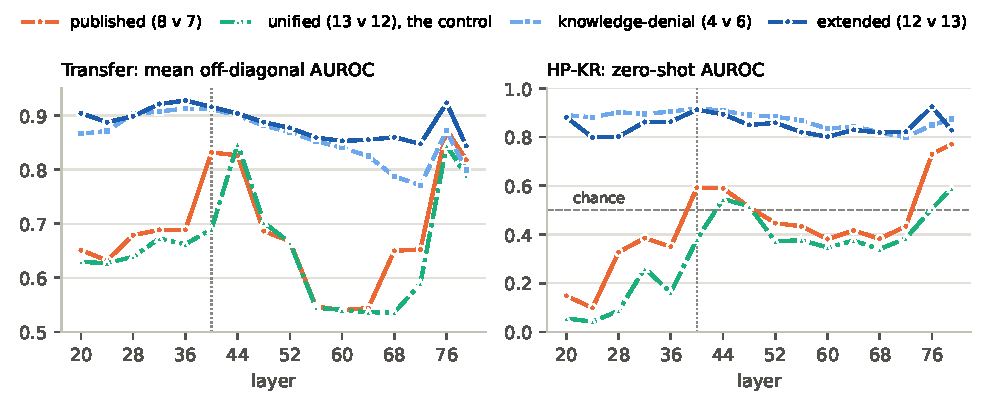
\includegraphics[width=\linewidth]{fig_widening.pdf}
\caption{The widening control across Pipeline~B's 16 layers: transfer (left) and HP-KR ranking (right).}
\label{fig:r-widening}
\end{figure}
% src: thesis/images/fig_widening.pdf, made by thesis_tools/figures/fig_widening.py from collaborator results/persona_depth/depth.csv @16def2de :: bank "ext", metric auroc, sources "transfer, off-diagonal mean" and "zero-shot, HP-KR", arms "deception axis (8v7)", "unified axis (13v12)", "knowledge-denial axis (4v6)", "extended axis (12v13)"; the script prints every plotted value

Widening with the sycophantic roles does not help. % interp: the averages and counts below
Averaged over the 16 layers, the unified contrast transfers at 0.6572 off-diagonal AUROC, below the 0.6860 of the published contrast it widens and far below the 0.8852 of the extended contrast. % src: thesis_tools/figures/fig_widening.py output :: depth.csv @16def2de, "transfer, off-diagonal mean", auroc, 16-layer averages: unified 0.6572, deception 0.6860, extended 0.8852
It transfers below the published contrast at 13 of the 16 layers; the exceptions are layers 44, 48 and 60. % src: fig_widening.py output :: "transfer: unified below published at 13/16 layers; not below at [44, 48, 60]"
On HP-KR it ranks below the published contrast at 15 of the 16 layers, the exception being layer 48, and it is above 0.5 at only four (44, 48, 76 and 79). % src: fig_widening.py output :: "HP-KR: unified below published at 15/16 layers; not below at [48]"; "unified above 0.5 at 4/16 layers: [44, 48, 76, 79]"
Its HP-KR AUROC averages 0.3338 over the 16 layers, against 0.4375 for the published contrast, 0.8726 for the knowledge-denial contrast and 0.8479 for the extended contrast. % src: fig_widening.py output :: depth.csv "zero-shot, HP-KR", auroc, 16-layer averages
So widening the bank is not what repairs HP-KR: widening with roles that lie by agreeable assertion makes it worse, and widening with roles that deny knowledge repairs it. % interp: unified 0.3338 < published 0.4375 < extended 0.8479 (HP-KR, 16-layer averages); the sycophancy contrast's own HP-KR values are in sec:r-zeroshot
Section~\ref{sec:r-interp} relates this to the register of the roles.
These averages share the sweep's limits: one run per layer, no dataset bootstrap, and 13 remote-pooled layers (Section~\ref{sec:r-adj-direction}). % src: collaborator deception_detection/scripts/layer_sweep.py @16def2de :: 39-40 (NEW_LAYERS, 13 of ALL_LAYERS, 16)

Pipeline~A ran the same three contrasts zero-shot on the kd bank at scores 2--3 (Pipeline~B keeps score 3), over its eleven datasets with mean pooling, and agrees on HP-KR. % src: lab PC C:/Users/user4/expLB/run-crossgen/kd11/banks/collab/matrices/mean_L{20,40,44}_s42.json (cache audit/cache/labpc/run-crossgen/kd11/banks/collab/matrices/) :: bank axes_collab_s23.pt; zeroshot directions contrast, contrast:unified, contrast:collab_extended (kd/personas/kd_role_groups_collab.json :: contrasts)
There the unified contrast reads 0.0600, 0.3358 and 0.5220 at layers 20, 40 and 44 (post hoc), against 0.1652, 0.5562 and 0.5733 for the published contrast and 0.8057, 0.8765 and 0.8491 for the extended contrast. % src: same cache :: zeroshot[direction].auroc at index 2 (harm-pressure-knowledge-report): contrast:unified 0.0600/0.3358/0.5220; contrast 0.1652/0.5562/0.5733; contrast:collab_extended 0.8057/0.8765/0.8491
Averaged over its eleven datasets, the unified contrast differs from the published one by $-0.0281$, $+0.0041$ and $+0.0143$ at the same layers. % src: same cache :: nanmean over the 11 datasets of zeroshot[contrast:unified].auroc minus zeroshot[contrast].auroc (computed)
These Pipeline~A values rest on a lab-only store, one seed, and no dataset bootstrap. % note: lab-only (cache md5 3d754892, 3f9fe86b, d5e15e03)

\subsection{The layer}
\label{sec:r-layer}

We fixed layer 40 before any 80-layer result existed; layers 36 and 44 are post hoc (Section~\ref{sec:m-layers}).
This subsection asks what that choice cost.
Figure~\ref{fig:r-depth} shows Pipeline~B's 16-layer sweep of transfer and of the zero-shot Liars' Bench average.

\begin{figure}[t]
\centering
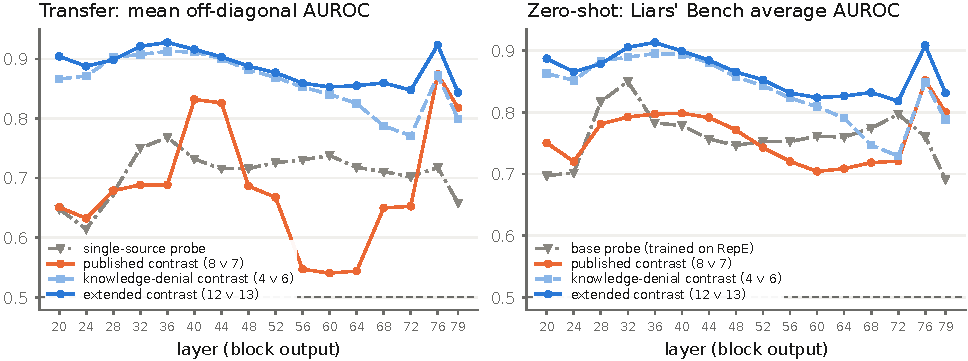
\includegraphics[width=\linewidth]{collab_fig_depth.pdf}
\caption{Transfer and the zero-shot Liars' Bench average across 16 layers, as plotted by Pipeline~B.}
\label{fig:r-depth}
\end{figure}
% src: thesis/images/collab_fig_depth.pdf = git cat-file blob 16def2deec34aeee532511df116adb7de5522ca7:src/probes/deception-detection/paper/generated/fig_depth.pdf (blob 873cb648abf3de3eca4a6adcfb02ab5d2b9ef0e8, 21,059 bytes = git cat-file -s; md5 1a45535b97c205e6af94f0b946db6479); plotted from results/persona_depth/depth.csv

\paragraph{Ranking peaks just before layer 40.}
For the extended contrast, both ranking measures peak at layer 36, which is post hoc. % src: collaborator persona_depth/depth.csv @16def2de :: arm "extended axis (12v13)", metric auroc: max of "transfer, off-diagonal mean" at L36 (0.9275) and of "zero-shot, Liars' Bench average" at L36 (0.9130)
There the extended contrast transfers at 0.9275 against 0.9158 at layer 40, and its Liars' Bench average is 0.9130 against 0.8990. % src: same file :: "transfer, off-diagonal mean" L36 0.92747, L40 0.91584; "zero-shot, Liars' Bench average" L36 0.913, L40 0.899 (stored at 4 decimals)
Keeping layer 40 therefore costs 0.0116 transfer AUROC. % src: same file :: 0.9274688514 - 0.9158352735 = 0.0116336 (computed)
The base probe peaks earlier still, at layer 32 (Section~\ref{sec:r-zeroshot}). % src: collaborator persona_depth/depth.csv @16def2de :: "zero-shot, Liars' Bench average", arm "base probe (RepE-trained)", auroc maximum at L32

\paragraph{Detection at the threshold peaks at layer 40.}
On HP-KR the knowledge-denial contrast reaches a balanced accuracy of 0.9102 at layer 40, against 0.7449 at layer 36 and 0.7571 at layer 44. % src: collaborator persona_depth/depth.csv @16def2de :: "zero-shot, HP-KR", arm "knowledge-denial axis (4v6)", metric balacc: L40 0.9102, L36 0.7449, L44 0.7571
From layer 36 to layer 76 it stays between 0.6941 and 0.9102; at layers 20--32 it is 0.4801--0.5490, and at layer 79 it is 0.5013. % src: same file and arm :: balacc L36-L76 min 0.6941 (L72), max 0.9102 (L40); L20 0.5331, L24 0.5490, L28 0.4801, L32 0.5043; L79 0.5013
So layer 40 is a narrow peak for detection inside a broad band where the contrast flags HP-KR's lies at all. % interp: balacc 0.9102 at L40 vs 0.7449 and 0.7571 either side; 0.6941-0.9102 over L36-L76
We kept layer 40: it is the pre-registered layer, and it is where the requirement that no other design meets, flagging HP-KR's lies at the threshold, is met best, at a ranking cost of 0.0116. % interp: the numbers of this and the previous paragraph; sec:r-hpkr reports the other designs at the threshold
Every layer of this sweep except 20, 40 and 44 rests on the uncommitted remote pooling code (Section~\ref{sec:m-transform}), and the sweep has one run per layer with no dataset bootstrap. % src: collaborator deception_detection/scripts/layer_sweep.py @16def2de :: 39-40

\paragraph{Pipeline~A: a plateau it cannot order.}
Pipeline~A's grid shows a plateau around layer 40 rather than a peak at it. % interp: the next two sentences
Over its eleven datasets, with mean pooling and the \texttt{paper} probe, the raw-activation probe transfers at 0.6818 at layer 32 and 0.6623 at layer 40. % src: run-crossgen/kd11/matrices/mean_L{32,40}_s42.json :: results[raw, paper].auroc, off-diagonal nanmean over 110 cells: 0.68177, 0.66230
On the kd bank at scores 2--3, the \texttt{axes} feature, the projections onto four contrast directions (Section~\ref{sec:m-features}), reads 0.6435 at layer 44 against 0.6304 at layer 40. % src: run-crossgen/kd11/banks/kd_s23/matrices/mean_L{44,40}_s42.json :: results[axes, paper].auroc, off-diagonal nanmean: 0.64350, 0.63040
These are one-seed means without a dataset bootstrap, so they show a plateau over roughly layers 32--44, not an order within it. % interp: gaps of 0.0195 and 0.0131, against the dataset-level intervals of sec:r-stats

\paragraph{Layers 20, 22 and 40.}
The two literature layers, 20 (Liars' Bench) and 22 (Apollo), are close but not shown to be equivalent. % interp: the next two sentences
Over the 17 methods whose result files hold both layers, the median gap between them is 0.0115 AUROC and the largest is 0.0370. % src: run-coords/q6_layers.json :: rows[*].gap_20_22 (17 non-null): median 0.011547, max 0.037019
On the nine labelled datasets, none of the four pre-registered equivalence tests keeps its 90\% dataset-bootstrap interval within $\pm0.02$; the intervals span $-0.0383$ to $+0.0335$. % src: run-coords/significance.json :: margin 0.02; comparisons[7]-[10] (Q6, kind equiv) equivalent_within_margin False; dataset_ci90 lows -0.0383 (comparisons[7]), highs up to +0.0335 (comparisons[8])
Moving to layer 40 matters more, and how much depends on the method.
Against the better of layers 20 and 22, layer 40 adds a median of $+0.0251$ AUROC for the ten raw-activation methods (range $-0.0157$ to $+0.0681$) and $+0.1135$ for the 13 persona methods (up to $+0.2335$). % src: run-coords/q6_layers.json :: rows[*].gap_40_minus_best_of_20_22; raw rows 0,3,6,9,16-21 (median 0.025100, min -0.015704, max 0.068146); persona rows 1,2,4,5,7,8,10-15,22 (median 0.113456, max 0.233504) (computed)
Comparing methods at layer 20 or 22 would therefore handicap the persona methods far more than the raw probes. % interp: medians +0.1135 vs +0.0251

\paragraph{Where each feature peaks.}
In Pipeline~A's sweep of the paper16 bank over the nine labelled datasets at full size (\texttt{mms} probe, mean pooling, off-diagonal mean over the 72 source--target pairs), the \texttt{axes} feature peaks at layer 44 (post hoc) at 0.7309, and the raw-activation probe peaks at layer 32 at 0.7167. % src: run-coords/layer_sweep_passB_mms.json :: pooling mean, probe mms, bank axes_vectors_s3_fp32.pt; sweep max axes L44 0.73089, raw L32 0.71673; run-coords/significance.json :: datasets (9; 9 x 8 = 72 pairs, computed)
It beats raw only at layers 36--48 (and, trivially, at layer 0). % src: same file :: axes > raw at layers [0, 36, 40, 44, 48]
The published method's own feature, \texttt{pc:deception}, beats raw at no layer under mean pooling; under last-token pooling it does so only at layers 0, 8 and 16, where raw itself reads 0.4962--0.6018. % src: same file :: pc:deception > raw at no layer; run-coords/layer_sweep_passB_last.json :: pc:deception > raw at [0, 8, 16], raw 0.49621, 0.51173, 0.60179
Best against best, the \texttt{axes} feature's lead over raw is $+0.0142$, with a 95\% dataset-bootstrap interval of $[-0.1123, +0.1613]$ ($p=0.8612$), so the ordering of the two peaks is not established. % src: run-coords/significance.json :: comparisons[0] "axes@44 vs raw@32, each at its best (mean)": diff 0.0142, dataset_ci95 [-0.1123, 0.1613], dataset_p 0.8612

\paragraph{The late layers.}
Both pipelines see transfer rise again near the last layers (Figures~\ref{fig:r-widening} and~\ref{fig:r-depth} show Pipeline~B's). % src: collaborator persona_depth/depth.csv @16def2de :: "transfer, off-diagonal mean", auroc, L72 -> L76: deception axis 0.6526 -> 0.8738, extended axis 0.8474 -> 0.9232; passA cache (below) :: axes L72 0.4846 -> L79 0.6656
In Pipeline~A's 200-row-per-dataset store, on five of its ten datasets (ID, CG, ai\_liar, roleplaying and mask), random directions gain $+0.1271$ AUROC between layers 72 and 79 (0.5133 to 0.6405; mean pooling, \texttt{paper} probe). % src: lab PC C:/Users/user4/expLB/run-crossgen/passA/matrices/mean_L{72,79}_s42.json (cache audit/p17/labcache/expLB/run-crossgen/passA/matrices/) :: results[random, paper].auroc, off-diagonal nanmean over instructed-deception, mask, convincing-game, ai_liar, roleplaying: L72 0.513344, L79 0.640472, gain 0.127127 (cache md5 = meta.json md5: L72 1975a8a4, L79 e8afc7d5)
On that reading the late rise looks like a property of the late layers, not of the personas. % interp: on the five datasets random directions gain +0.1271 and the axes feature +0.1108 (0.6384 -> 0.7492, same cache) between L72 and L79
It does not hold on the store's full ten datasets. % interp: the next sentence
There, random directions fall from 0.5718 to 0.5498 between layers 72 and 79, while the \texttt{axes} feature rises from 0.4846 to 0.6656. % src: same cache :: off-diagonal nanmean over all 10 datasets, paper probe: random L72 0.571846, L79 0.549840; axes L72 0.484638, L79 0.665556
The five-dataset reading also overstates the level: at layer 40 the raw-activation probe transfers at 0.8195 on those five datasets but at 0.6760 on all ten. % src: same cache, mean_L40_s42.json :: results[raw, paper].auroc off-diagonal nanmean, 5 datasets 0.81952, 10 datasets 0.67600 (cache md5 83ccac49)
We therefore leave the late rise unexplained; it rests on a lab-only store and one seed. % interp: the two readings disagree

\subsection{The token read and pooling}
\label{sec:r-token}

Except where last-token pooling is named, every result above reads a response through the mean of its token activations, which is also how a persona vector is built (Equation~\ref{eq:m-persona}).
Because a contrast score is a dot product, the score can also be taken at each token and the per-token scores reduced to one number in other ways. % src: collaborator persona_positions_L40/summary.md @16def2de :: "The data are exact" (per-token projections average to the pooled projection)
We call each such reduction a \emph{token read}: the mean over the response tokens, the mean of the top 10\% of token scores, the maximum, the first or last response token, or the last prompt token before the reply. % src: collaborator persona_positions_L40/summary.md @16def2de :: table of reads (mean; max, top-10% mean; first, last; before the reply = the last prompt token)
Table~\ref{tab:r-reads} compares the six reads for the extended contrast in Pipeline~B, zero-shot, averaged over the five Liars' Bench datasets at the Alpaca threshold. % src: collaborator persona_positions_L40/reads_summary.csv @16def2de :: axis extended; averages over CG, HP-C, HP-KR, IT, ID (mean read 0.899 = mean of reads.csv rows 0.9123, 0.7116, 0.9124, 0.9803, 0.9784)

\begin{table}[t]
\centering
\footnotesize
\caption{Six token reads of the extended contrast, averaged over the five Liars' Bench datasets.}
\label{tab:r-reads}
\begin{tabular}{p{27mm}ccccccccc}
\hline
 & \multicolumn{3}{c}{Layer 20} & \multicolumn{3}{c}{Layer 40} & \multicolumn{3}{c}{Layer 44 (post hoc)} \\
Read & AUROC & BA & Recall & AUROC & BA & Recall & AUROC & BA & Recall \\
\hline
Mean (default) & 0.8868 & 0.5914 & 0.1872 & 0.8990 & 0.6939 & 0.4129 & 0.8841 & 0.6663 & 0.3503 \\
Top-10\% mean & 0.8727 & 0.6635 & 0.3479 & 0.9075 & 0.7372 & 0.5306 & 0.9074 & 0.7153 & 0.4703 \\
Maximum & 0.8581 & 0.6594 & 0.3361 & 0.9095 & 0.7497 & 0.5480 & 0.9140 & 0.7011 & 0.4176 \\
First response token & 0.7531 & 0.6048 & 0.3343 & 0.8631 & 0.6059 & 0.2270 & 0.8757 & 0.5683 & 0.1397 \\
Last response token & 0.8425 & 0.6445 & 0.3120 & 0.8797 & 0.6556 & 0.4221 & 0.8815 & 0.6361 & 0.3522 \\
Token before the reply & 0.7393 & 0.6275 & 0.4149 & 0.8254 & 0.6515 & 0.3829 & 0.8222 & 0.6556 & 0.3274 \\
\hline
\end{tabular}
\end{table}
% src: collaborator results/persona_positions_L{20,40,44}/reads_summary.csv @16def2de :: rows axis = extended, reads mean, top10, max, first, last, pre; columns auroc, balacc, recall. BA is balanced accuracy at the threshold that flags 1% of Alpaca.
% note: the CSV stores 4 decimals and drops trailing zeros (0.899, 0.548, 0.914, 0.227, 0.312); they are printed here as 0.8990, 0.5480, 0.9140, 0.2270, 0.3120, the same values.

For ranking, the mean is the best read at layer 20, and at layers 40 and 44 the two peak reads, the maximum and the top-10\% mean, lead it by at most 0.0299 AUROC. % src: Table tab:r-reads source :: L20 mean 0.8868 highest; L40 max 0.9095 - mean 0.899 = 0.0105; L44 max 0.914 - mean 0.8841 = 0.0299 (computed)
For detection at the threshold, both peak reads beat the mean at all three layers. % src: same :: balacc top10 / max vs mean: L20 0.6635 / 0.6594 vs 0.5914; L40 0.7372 / 0.7497 vs 0.6939; L44 0.7153 / 0.7011 vs 0.6663
Which peak read is better depends on the layer: of the two, the top-10\% mean has the higher balanced accuracy and recall at layers 20 and 44, and the maximum at layer 40, with 0.7497 and 0.5480 against 0.7372 and 0.5306. % src: same :: balacc and recall per layer (L20 top10 0.6635/0.3479 vs max 0.6594/0.3361; L44 top10 0.7153/0.4703 vs max 0.7011/0.4176; L40 max 0.7497/0.548 vs top10 0.7372/0.5306)
The maximum is the less stable read: at layer 40 it lowers RepE's balanced accuracy from 0.9982 under the mean to 0.6382, where the top-10\% mean keeps 0.9582. % src: collaborator persona_positions_L40/reads.csv @16def2de :: axis extended, dataset repe_honesty__plain, balacc: mean 0.9982, max 0.6382, top10 0.9582
The final design keeps the mean, which is how the persona vectors are built and which ranks best at layer 20; for detection at a threshold, a peak read is the better choice, and neither peak read wins at every layer. % interp: the three sentences above

\paragraph{Where the read is taken.}
The persona direction's sign does not hold at every token position. % interp: the values below
Pipeline~B also scored the contrasts at the single token of the Follow-Up Probe (Section~\ref{sec:r-problem}), at layer 20. % src: collaborator persona_ood_followup_L20/summary.md @16def2de :: lines 3-7 (activation at the prefilled "No"); zero_shot.csv :: layer 20
There the published contrast falls on IT from 0.988 on response tokens to 0.165, and the knowledge-denial contrast falls on HP-KR from 0.890 to 0.237. % src: collaborator persona_ood_ext_L20/zero_shot.csv and persona_ood_followup_L20/zero_shot.csv @16def2de :: insider_trading_cadenza__plain auroc_axis 0.98790 -> 0.16501; harm_refusal_knowledge_report__plain auroc_denial_axis 0.88993 -> 0.23673
The extended contrast's Liars' Bench average falls from 0.8868 to 0.5518. % src: same two files :: auroc_ext_axis, mean over CG, HP-C, HP-KR, IT, ID: 0.88683 (response tokens), 0.55183 (follow-up token) (computed)
So the knowledge-denial repair of HP-KR is a property of the response tokens, where the denial is written. % interp: 0.890 -> 0.237 on HP-KR
The token before the reply reads the prompt more than the response. % interp: the values below
In Pipeline~B it gives the extended contrast an AUROC of 1.0 on CG at layers 40 and 44 and on RepE at all three layers, while on HP-KR it reads 0.3855 at layer 20. % src: collaborator persona_positions_L{20,40,44}/reads.csv @16def2de :: axis extended, read pre: convince_me__plain auroc 1.0 (L40, L44), 0.8714 (L20); repe_honesty__plain 1.0 (L20, L40, L44); harm_refusal_knowledge_report__plain 0.3855 (L20)
Pipeline~A's prompt-only store agrees: reading only the prompt tokens, a raw-activation probe reaches an in-distribution AUROC of 1.0 on CG at layers 20, 40 and 44, and on sandbagging\_v2 at layers 40 and 44 (mean pooling). % src: lab PC C:/Users/user4/expLB/run-crossgen/passP/summary.json (cache audit/p17/labcache/expLB/run-crossgen/passP/summary.json, md5 9d95c403) :: records[pooling=mean, feature=raw, probe=paper].diagonal: convincing-game 1.0 at L20, L40, L44; sandbagging_v2 1.0 at L40, L44 (0.999 at L20)
Off-diagonal over the store's ten datasets, the same prompt-only probe transfers at 0.5584, 0.5687 and 0.5697 at layers 20, 40 and 44. % src: same :: records[mean, L20/L40/L44, raw, paper].offdiag_mean_10 0.55838, 0.56870, 0.56971
On these datasets the instruction to lie is already visible before the model answers, so a read taken there measures the instruction as much as the lie. % interp: prompt-only in-distribution 1.0 on CG and sandbagging_v2; pre-token 1.0 on CG and RepE; this rests on a lab-only store and one seed

\paragraph{Pipeline~A's per-token results.}
Pipeline~A's per-token study used the paper16 deception contrast and one AUROC over its whole per-token store. % src: src/assistant_axis_ndif/14_pertoken.py :: 122-131 ("pooled AUROC over the whole corpus, by aggregation (zero-shot, no training)"); run-coords/pertoken_q8.json :: axis deception, bank axes_vectors_s3_fp32.pt
Zero-shot, the top-10\% read beats the mean by $+0.1027$ at layer 20, but by only $+0.0046$ at layer 40. % src: run-coords/pertoken_q8.json :: aggregations[layer 20] top10pct 0.79815 - mean 0.69544; aggregations[layer 40] top10pct 0.76985 - mean 0.76524 (computed)
Trained leave-one-dataset-out over nine datasets, the best probe on the pooled mean beats the best probe trained on single tokens at all six layers, by 0.0276 to 0.0604. % src: run-coords/q8_trained_pertoken.json :: summary[layer].best_pooled.auroc_mean minus best_token.auroc_mean: L20 0.8570-0.7966, L22 0.8544-0.8047, L28 0.8764-0.8279, L40 0.8826-0.8526, L44 0.8783-0.8507, L48 0.8739-0.8294 (computed; min 0.0276 at L44, max 0.0604 at L20)
The two pipelines differ in contrast, bank, dataset set and metric, so their effect sizes are not comparable; both find the largest gain from a peak read at layer 20, on balanced accuracy in Pipeline~B and on AUROC in Pipeline~A. % interp: Pipeline B top10 - mean balacc +0.0721 (L20), +0.0433 (L40), +0.0490 (L44); Pipeline A top10 - mean AUROC +0.1027 (L20), +0.0046 (L40)

\paragraph{Pooling at 70B.}
Pooling also changes whether persona features beat the raw probe at 70B.
On the paper16 bank, over five datasets (ID, CG, ai\_liar, roleplaying and mask) at $k=3$ with one seed and the \texttt{paper} probe, we take at each layer the best of the four persona features (\texttt{axes}, \texttt{pc:deception}, \texttt{pc:unified} and \texttt{pc:unified@2}) and compare its off-diagonal AUROC with the raw probe's, averaged over 21 layers. % src: lab PC C:/Users/user4/expLB/run-crossgen/scale_70b_paper16fp32/matrices/{mean,last}_L*_s42.json (cache audit/p17/labcache/expLB/run-crossgen/scale_70b_paper16fp32/matrices/, 42 files, each md5 = its meta.json md5) :: bank axes_vectors_s3_fp32.pt (bank_name paper16_70b_fp32), k 3, datasets instructed-deception, mask, convincing-game, ai_liar, roleplaying; results[feature, paper].auroc off-diagonal nanmean; best = max over axes, pc:deception, pc:unified, pc:unified@2 (the definition of audit/scripts/p12_kd_scale_ladder.py :: 59-73)
Under mean pooling the best feature trails the raw probe by 0.0116 and is ahead at only 9 of the 21 layers; under last-token pooling it leads by $+0.0100$ and is ahead at 14. % src: same cache :: mean: mean(best) - mean(raw) = -0.011602, per-layer best > raw at 9/21; last: +0.009994, 14/21 (computed)
Against the dataset-PCA control at the same $k$ it leads under both poolings, by $+0.0605$ and $+0.0712$. % src: same cache :: mean(best) - mean(datapca): mean pooling 0.060470, last 0.071171 (computed)
The best feature at each layer is chosen post hoc, so these are optimistic readings, and there is no dataset bootstrap. % interp: per-layer max over four features; one seed
% note: run-crossgen/scale_70b/ is NOT used: its layer 40 comes from the paper16 bank and its other 20 layers from the kd bank under one label (verified: zero-shot contrast AUROCs at L20 and L44 equal run-crossgen/kd11/banks/kd exactly, at L40 match run-crossgen/kd11/matrices to within 0.0003; both bank fields read axes_vectors_s3.pt / paper16_70b). Over that mixed store max(axes, pc:deception) - raw under mean pooling reads +0.0070 (11/21).
Section~\ref{sec:r-scale} gives the comparison across model sizes.

\subsection{Approaches that did not work}
\label{sec:r-failed}

Four further attempts did not work, and one test gave opposite answers under the two poolings.
For two of them, D3 and D10, the result files are not in the repository, so we quote their numbers from the written report of those runs and cannot re-derive them. % src: git ls-tree -r --name-only on 16def2de, e917ecd3 and origin/feat/persona-pc-ood, searched for inlp, aisi, dann (no match, 2026-09-25); git show -s 148ddeb9 :: "The INLP experiment remains uncommitted."; owner's statement, 2026-09-25

\paragraph{An on-policy base probe (D3).}
RepE's lies are written under an instruction to lie, which is off-policy for the lies in the evaluation datasets. % src: full paper draft for this experiments/report.pdf :: p.37 (Section 4.2.2, D3; printed page 23)
D3 trained the base probe instead on 3{,}285 of the model's own belief-labelled responses, 1{,}634 lies and 1{,}651 honest answers, from the UK AI Security Institute's lie-detection rollouts \parencite{aisi2026liedetection}. % src: full paper draft for this experiments/report.pdf :: p.37 (Section 4.2.2; printed page 23); dataset reference p.62 (bibliography [30])
It raised the Liars' Bench average AUROC over D2 by 0.100, with a paired interval of $[0.086, 0.113]$. % src: full paper draft for this experiments/report.pdf :: p.44 (Section 5.2.1; printed page 30)
It did not close the gap to the persona contrasts: the extended contrast still led it by 0.021 $[0.006, 0.035]$ at layer 40 and by 0.105 at layer 20, and at layer 44 the interval included zero. % src: full paper draft for this experiments/report.pdf :: p.44 (Section 5.2.1; printed page 30)
Like D2, it flagged none of HP-KR's lies at the Alpaca threshold, with a balanced accuracy of 0.500 despite an AUROC of 0.935 at layer 40. % src: full paper draft for this experiments/report.pdf :: p.45 (Table 5.1, row D3; printed page 31)

\paragraph{A learned subspace (D10).}
If a low-dimensional subspace is what lets the persona method transfer, a subspace learned from labels might do the same. % src: full paper draft for this experiments/report.pdf :: p.39 (Section 4.2.5; printed page 25)
D10 learned one with iterative nullspace projection (INLP) \parencite{ravfogel2020null} on RepE: each round trains a probe with every earlier round's direction projected out, and the first $k$ directions span the subspace. % src: full paper draft for this experiments/report.pdf :: p.39 (Section 4.2.5; printed page 25)
It was run at layer 20 on the published persona run's activations, with transfer averaged over the 25 cells that exclude RepE as a test set. % src: full paper draft for this experiments/report.pdf :: p.45 (Section 5.2.4; printed page 31)
At rank 1 INLP transferred at 0.632, against 0.634 for the raw-activation probe, and at every rank from 2 to 50 it transferred worse, at 0.530--0.583. % src: full paper draft for this experiments/report.pdf :: p.45 (Section 5.2.4; printed page 31)
At those ranks its standard deviation across training sets was 0.151--0.293, against 0.180 for the raw-activation probe and 0.032 for the persona components. % src: full paper draft for this experiments/report.pdf :: p.45 (Section 5.2.4, "sensitivity to the training set"; printed page 31); p.48 (Figure 5.4, right panel "train-set sensitivity", axis "std across training sets"; printed page 34)
A label-free basis of the same number of RepE principal components beat the INLP basis at every rank from 2 to 50, though not at rank 1. % src: full paper draft for this experiments/report.pdf :: p.45 (Section 5.2.4; printed page 31: "beats the supervised INLP basis at every rank"); p.48 (Figure 5.4, both AUROC panels: at k = 1 the PCA point lies below the INLP point; printed page 34), so the text's "every rank" holds only from rank 2
So supervision picked the directions that separate the training set, which are the ones that fail to transfer. % interp: INLP 0.530-0.583 vs raw 0.634 at ranks 2-50; PCA basis above INLP at ranks 2-50 (report p.45, Figure 5.4 p.48)

\paragraph{Domain-adversarial training.}
We also tried domain-adversarial training (DANN) \parencite{ganin2016domain}, which trains features so that an adversarial classifier cannot tell the training domains apart. % src: owner's statement, 2026-09-25 (DANN tried and did not work)
It did not work either. % src: owner's statement, 2026-09-25
No code, result file or number from the attempt is in the repository or in the written report, so we give no numbers for it. % src: git ls-tree search of 16def2de, e917ecd3, origin/feat/persona-pc-ood for "dann" (no match, 2026-09-25); full paper draft for this experiments/report.pdf :: text search for DANN/adversarial (no match, 2026-09-25)

\paragraph{Growing the text-matched slice.}
The text-matched slice has 258 rows because HP-KR holds only 134 honest denials by a model that does not know the answer (Figure~\ref{fig:m-hpkr}). % src: kd/scripts/gen_hpkr_denial.py :: 4-8 (docstring: slice capped at 258 rows by the 134-row cell); thesis_tools/figures/fig_hpkr_cells.py :: count (F,F,T) = 134
To grow it, we put WMDP items that the model answers wrongly under a neutral prompt into HP-KR's own template, expecting it to deny knowing them, and predicted a denial rate of at least 0.70 on a first 20 items, with the route to be abandoned below 0.40. % src: kd/scripts/gen_hpkr_denial.py :: 10-21 (312 wrong items; HP-KR's own template; "Predicted >= 0.70; below 0.40 the route yields nothing"), 203-205 (PASS if rate >= 0.70, MARGINAL if >= 0.40, else GATE FAILED)
The model denied knowledge on 5 of the 20 (0.250). % src: log-only lab PC C:/Users/user4/expLB/logs/hpkr_denial_smoke.log :: GATE line "GATE  denial rate = 5/20 = 0.250" followed by "GATE FAILED"
With HP-KR's neutral control template it denied on 3 of 20 (0.150). % src: log-only lab PC C:/Users/user4/expLB/logs/hpkr_denial_control.log :: GATE line "GATE  denial rate = 3/20 = 0.150"
Selecting instead the items the model answered with the least confidence, it denied on 5 of the 12 items that completed (0.417). % src: log-only lab PC C:/Users/user4/expLB/logs/hpkr_denial_margin.log :: line 1 "selected 20 items (select=margin, template=harmful)"; GATE line "GATE  denial rate = 5/12 = 0.417"
The first two routes fell below the 0.40 floor, the third reached only the band between 0.40 and 0.70, and the slice stayed at 258 rows. % src: log-only lab PC C:/Users/user4/expLB/logs/hpkr_denial_{smoke,control}.log :: "GATE FAILED" after each GATE line; margin: 0.417 lies in the MARGINAL band of gen_hpkr_denial.py :: 205 (log line not printed in the audit extract audit/phase2/out/P6/P6_lab_a.txt)
The model mostly claimed to know answers it got wrong, which suggests that the cell limiting the slice is small because the model rarely admits ignorance. % interp: 15 of 20 primary items not denied (5/20 denied)

\paragraph{Reading an inverted axis as a signal.}
On \texttt{sycophancy\_mt} the paper16 deception direction scores below 0.5 (Section~\ref{sec:r-cap}), which raised the possibility of a real signal with a flipped sign. % src: run-crossgen/kd11/matrices/mean_L40_s42.json :: zeroshot contrast auroc[10] 0.40892, PC1 auroc[10] 0.37396 (sycophancy_mt)
If so, a probe on the \texttt{axes} feature trained on \texttt{sycophancy\_mt} (paper16 bank, \texttt{paper} probe, one seed), with its scores inverted, should transfer to the other ten datasets better than a probe on random directions. % src: run-crossgen/kd11/matrices/{mean,last}_L*_s42.json :: results[axes|random, paper].auroc, row sycophancy_mt (index 10), off-diagonal mean; inverted = 1 - AUROC
Under mean pooling it does so at only 7 of 21 layers; at layer 40 it reads 0.6213 against 0.6327 for random directions. % src: same, mean pooling :: inverted axes > random at 7 of 21 layers (computed); L40 axes row mean 0.37873 (inverted 0.62127), random 0.63269
Under last-token pooling it does so at 18 of 21 layers, and at layer 40 it reads 0.7356 against 0.4786. % src: same, last pooling :: inverted axes > random at 18 of 21 (computed); L40 axes 0.26444 (inverted 0.73556), random 0.47862
The test passes under one pooling and fails under the other, so we draw no conclusion from it. % interp: 7/21 (mean) vs 18/21 (last); one seed, paper16 bank, k = 5

The sarcasm bank designed to separate deceptive intent from wording was never built beyond its pilot (Section~\ref{sec:r-sarcasm}). % src: cap/docs/SARCASM_DESIGN.md :: 1-3 ("design v2 ... Status: revised, not built"); chapter_5.tex :: 486 (the sarcasm pilot builds no vectors)

\subsection{Adjustments to the claims}
\label{sec:r-claims}

The 16-layer sweep and our audit of both pipelines corrected several claims first made from fewer layers or fewer datasets.
Each is stated here in its corrected form, with the result that corrects it.
\begin{itemize}
\item \textbf{The extended contrast beats the raw-activation probe on every held-out dataset.} % src: the claim as first made and as corrected: full paper draft for this experiments/report.pdf :: p.52 (Section 5.3.6; printed page 38)
It does so only at layers 20--48 and 76--79; from layer 52 to 72 it trails on HP-C, and at layers 60 and 68 also on HP-KR. % src: collaborator persona_ood_ext_L*/matrix_ext_axis1.csv and matrix_baseline.csv @16def2de :: per test-set column, mean over the five other training rows (computed): ext <= baseline on HP-C at L52-L72, on HP-KR at L60 and L68
\item \textbf{One direction beats the components at every layer.} % src: full paper draft for this experiments/report.pdf :: p.52 (Section 5.3.6; printed page 38)
It does so at 13 of 16 layers (Section~\ref{sec:r-adj-direction}). % src: collaborator persona_ood_ext_L*/summary.csv @16def2de :: ext_axis1 - ext_pc3 off_diagonal_mean positive at 13 of 16 (computed)
\item \textbf{The base probe inverts on IT.} % src: full paper draft for this experiments/report.pdf :: p.44 (Section 5.2.1, D2 'inverts on insider trading (0.338)'); p.52 (Section 5.3.6, 'the base probe inverts on more datasets than first reported')
At layer 40 it does; across the sweep it also inverts on HP-C at layer 20 and on HP-KR at layers 20--28, and on IT at every layer from 36 to 79. % src: collaborator persona_ood_ext_L*/zero_shot_operating.csv @16def2de :: arm "base probe (RepE-trained)", threshold_source control, auroc < 0.5: HP-C L20 (0.4708); HP-KR L20, L24, L28 (0.109, 0.0657, 0.491); IT L36-L79 (0.2408-0.3378)
\item \textbf{The sycophancy contrast inverts on HP-KR at every layer.} % src: full paper draft for this experiments/report.pdf :: p.52 (Section 5.3.6; printed page 38)
It is below 0.5 at 15 of 16 layers and reaches 0.5073 at layer 48. % src: collaborator persona_ood_ext_L*/zero_shot.csv @16def2de :: harm_refusal_knowledge_report__plain, auroc_syc_axis (L48 0.50727; below 0.5 at the other 15 layers)
\item \textbf{From layer 36 the base probe ranks HP-KR better than any contrast.} % src: the claim at collaborator paper/sections/introduction.tex @16def2de :: 68-70
It does so at 8 of the 12 layers from 36; it trails the best contrast at layer 44 (0.8283 against 0.9077), 48 (0.8373 against 0.8903), 52 (0.8773 against 0.8834) and 76 (0.8382 against 0.9249). % src: collaborator persona_depth/depth.csv @16def2de :: "zero-shot, HP-KR", auroc, base probe vs max of the 8v7, 4v6, 12v13 arms (computed)
\item \textbf{On the datasets other than HP-KR, the extended contrast beats the published one by at least 0.026 at every layer.} % src: the claim at collaborator paper/sections/limitations.tex @16def2de :: 17-21
The 0.026 is computed with HP-KR included, where the smallest margin is 0.0257 at layer 79. % src: collaborator paper/generated/numbers.tex @16def2de :: 1113 (depth-ext-over-dec-min 0.026); persona_ood_ext_L79/summary.csv :: ext_axis1 - axis1 off_diagonal_mean 0.84363 - 0.81792 = 0.02571 (minimum over 16 layers, computed)
Without HP-KR the margin is $-0.0108$ at layer 20 and below 0.026 at 8 of the 16 layers. % src: collaborator persona_ood_ext_L*/summary.csv @16def2de :: ext_axis1 - axis1, off_diagonal_mean (min 0.02571 at L79) and off_diagonal_excl_hpkr (L20 -0.01083; < 0.026 at 8 of 16) (computed)
\item \textbf{The wording-controlled test, feigned against sincere ignorance where both sides deny, has not been run.} % src: the claim at collaborator paper/sections/limitations.tex @16def2de :: 10-11 ("we have not run it"); full paper draft for this experiments/report.pdf :: p.56 (Section 5.6.3; printed page 42)
It has been run, and Section~\ref{sec:r-hpkr} reports it. % src: lab PC C:/Users/user4/expLB/run-crossgen/kd11/banks/collab/matrices/mean_L{20,40,44}_s42.json (cache audit/cache/labpc/run-crossgen/kd11/banks/collab/matrices/) :: zeroshot[contrast:knowledge_denial].auroc[3] (harm-pressure-kr-matched, the text-matched slice) 0.3932 / 0.4989 / 0.4825
\item \textbf{A probe trained on several pooled datasets is not compared.} % src: the claim at collaborator paper/sections/limitations.tex @16def2de :: 42-44; full paper draft for this experiments/report.pdf :: p.57 (Section 5.6.3; printed page 43)
Pipeline~B's own pooled leave-one-out runs make that comparison (Section~\ref{sec:r-pooled}). % src: git ls-tree 16def2de src/probes/deception-detection/results/ :: loo_L20, loo_L40
\item \textbf{For detection at the threshold, the top-10\% read is best.} % src: the claim at collaborator paper/sections/appendix.tex @16def2de :: 108 ("the top-10% read is best")
At layer 40 the maximum is better on balanced accuracy and recall (Section~\ref{sec:r-token}). % src: collaborator persona_positions_L40/reads_summary.csv @16def2de :: extended max 0.7497/0.548 vs top10 0.7372/0.5306
\item \textbf{Our own notes.}
The one-direction margin over the components without HP-KR is not ``within $\pm0.06$'', as our notes first said (Section~\ref{sec:r-d4} gives its range). % src: the claim at kd/docs/FINDINGS.md :: F-117; corrected value from collaborator persona_ood_ext_L56/summary.csv @16def2de :: ext_axis1 - ext_pc3, off_diagonal_excl_hpkr 0.86699 - 0.80373
The explanation of the late-layer rise holds only on five of the ten datasets (Section~\ref{sec:r-layer}). % src: the claim at kd/docs/FINDINGS.md :: F-120; corrected from passA matrices (cache audit/p17/labcache/expLB/run-crossgen/passA/matrices/)
Our notes compared the two poolings at 70B on a store whose layers mix the paper16 and kd banks under one label; Section~\ref{sec:r-token} gives the comparison on paper16 alone. % src: the claim at kd/docs/FINDINGS.md :: F-101; verified mixed: lab PC C:/Users/user4/expLB/run-crossgen/scale_70b/matrices/mean_L{20,40,44}_s42.json (cache audit/p17/labcache/expLB/run-crossgen/scale_70b/matrices/) zero-shot contrast AUROCs equal run-crossgen/kd11/banks/kd at L20 and L44 and run-crossgen/kd11/matrices at L40 (to within 0.0003)
Layers 20 and 22 are not shown equivalent within the pre-registered $\pm0.02$, a margin that our results notes had widened to $\pm0.04$ (Section~\ref{sec:r-layer}). % src: the widened claim at docs/thesis/persona-coordinates-70b-results.md :: 762-764 (original text, kept below its DF-63 correction block at 745-761); run-coords/significance.json :: margin 0.02, comparisons[7]-[10] equivalent_within_margin False
\end{itemize}

% ===== PART W6a (verified) =====
% ---------------------------------------------------------------------
% Part W6a -- Section 5.4 Statistical Analysis (plan rows 9.1-9.9, thesis_tools/planning/CH5_RESULTS_PLAN.md)
% Every number was re-read from its raw file on 2026-09-25. Owner (Pipeline A) files: asix working tree, or the lab-PC
% caches under audit/cache/labpc/ and audit/p17/labcache/ (lab-only; re-checked on the lab PC in the final session).
% Collaborator (Pipeline B) files: git show 16def2de:src/probes/deception-detection/results/<path>.
% ---------------------------------------------------------------------
\section{Statistical Analysis}
\label{sec:r-stats}

This section reports what the tests of Section~\ref{sec:m-stats} show when they are applied to the results of this chapter.
The two pipelines test differently.
Pipeline~A resamples datasets as well as rows and corrects for multiple testing. % src: src/assistant_axis_ndif/27_crossgen.py :: 779-827 (dataset bootstrap per block, BH within each block); src/assistant_axis_ndif/23_significance.py :: 12-20, 288-293
Pipeline~B reports 95\% stratified bootstrap intervals over the examples of each dataset, from 1{,}000 resamples, and never resamples datasets. % src: collaborator paper/sections/setup.tex @16def2de :: 39-40; collaborator deception_detection/scripts/persona_ood.py @16def2de :: 409-439 (bootstrap_delta resamples the rows of one test set), 572-574 ("a stratified bootstrap over examples"); git grep over 16def2de deception_detection/ and paper/sections/ finds no dataset-level bootstrap and no Benjamini-Hochberg step (checked 2026-09-25)
Every Pipeline~B interval in this chapter is therefore a row-level interval: it says whether a number is stable over the rows of the datasets studied, not whether it would hold on other datasets. % interp: from the two bootstrap definitions (src/assistant_axis_ndif/23_significance.py :: 12-20; persona_ood.py :: 572-574); collaborator paper/sections/limitations.tex @16def2de :: 52 ('Our bootstrap intervals resample examples, not models or prompts')

\paragraph{How wide nine to eleven datasets make an interval.}
The ten train-one-test-all significance files of Pipeline~A that we cached from the lab store hold 65{,}388 dataset-level tests between them. % src: lab PC C:/Users/user4/expLB/run-crossgen/**/significance.json (cache audit/cache/labpc/run-crossgen/**/significance.json, 10 files) :: len(tests) summed = 65,388, computed 2026-09-25; blocks hold 9, 10 or 11 datasets (pairs 72/90/110)
The median half-width of their 95\% dataset-bootstrap intervals is 0.1252 AUROC, and the 90th percentile is 0.1862. % src: same 10 files :: tests[].dataset_ci95, (hi - lo) / 2, median 0.12515, 90th percentile 0.18624, computed
Only 13.9\% of the tests show an effect larger than the half-width of their own interval, and 166 of them (0.25\%) clear Benjamini--Hochberg correction. % src: same :: |diff| > half-width in 13.91% of tests; significant_datasets true in 166, computed
Of those 166, 122 are a persona feature beating its random-projection control, 33 are a control (\texttt{random}, \texttt{random@2} or \texttt{datapca@2}) losing to \texttt{raw}, 6 are a persona feature beating \texttt{datapca}, and 5 compare a persona feature with \texttt{raw}. % src: same :: comparison field of the 166 clearing tests, computed (persona - random 122, all positive, one of them 'axes - random' with axes 4-d and random k=5; control - raw 33, all negative; persona - datapca 6; persona - raw 5)
Four of those five are \texttt{pc:kd\_assertion} beating \texttt{raw} on the kd bank (once at layer 68 with answers scored 3, three times at layer 40 with scores 2--3), which Section~\ref{sec:r-transfer} reports; the fifth is \texttt{pc:deception} on the own100 bank losing to \texttt{raw}, by $-0.1524$ at layer 20 (last-token pooling, \texttt{mms} probe, the nine datasets without \texttt{sycophancy\_mt}). % src: cache audit/cache/labpc/run-crossgen/kd11/banks/kd/significance.json (1 test) and kd11/banks/kd_s23/significance.json (3 tests) :: 'pc:kd_assertion - raw', diff +0.1497 (kd, block "10", mean, L68, paper) to +0.1771 (kd_s23, block "9", last, L40, lr_reg10); kd bank file axes_vectors_s3.pt, kd_s23 axes_vectors_s23.pt; audit/cache/labpc/run-crossgen/banks/own100/significance.json :: block "9" (72 pairs, 9 datasets), last, L20, mms, 'pc:deception - raw', diff -0.1524, q 0.0474
None of the six wins over \texttt{datapca} is at a pre-registered layer: five are \texttt{pc:unified@2} on the own100 bank at layers 68 and 72, and one is \texttt{pc:knowledge\_denial} on the kd bank (scores 2--3) at layer 0. % src: audit/cache/labpc/run-crossgen/banks/own100/significance.json :: block "9", mean, L68 (lr_reg10, mms, paper), L72 (lr_reg10, paper), 'pc:unified@2 - datapca@2'; kd11/banks/kd_s23/significance.json :: block "9", last, L0, paper, 'pc:knowledge_denial - datapca' +0.0894
The copies of these files in the repository are older and hold smaller families, so this census uses the lab store's copies. % src: run-crossgen/kd11/significance.json (git, 4,032 tests) vs its cache (4,788); run-crossgen/significance.json (git, 192 tests) vs its cache (4,788); all ten git copies are subsets of their caches, and the shared tests agree in diff and dataset_ci95 (checked 2026-09-25)

The settings this chapter reports most often give a sharper picture.
Restricted to persona features against \texttt{raw} at layers 20, 40 and 44 (44 post hoc), with mean pooling and the \texttt{paper} probe, there are 276 tests across the ten files' banks and dataset blocks. % src: same 10 cached files :: comparison '<persona feature> - raw', layer in {20, 40, 44}, pooling mean, probe paper; count 276, computed
Their median absolute difference is 0.0440, but their median signed difference is $-0.0263$: only 95 of the 276 are positive, and none clears correction. % src: same 276 tests :: median |diff| 0.04400, median diff -0.02630, diff > 0 in 95, significant_datasets true in 0, computed
Their median interval half-width is 0.1325, three times the median absolute difference. % src: same :: median (hi - lo) / 2 = 0.13250, computed
At layer 40 alone, the 92 such tests have a median signed difference of $-0.0051$; 44 are positive, and none clears. % src: same, layer 40 only :: n 92, median diff -0.0051, 44 positive, 0 significant, computed
So the typical persona-versus-\texttt{raw} difference is not an advantage hidden by noise. % interp: median signed difference -0.0263, 95 of 276 positive
It is usually no advantage at all, and nine to eleven datasets cannot resolve it either way. % interp: median half-width 0.1325 against median |difference| 0.0440; 0 of 276 clear

\paragraph{The replicated method at 70B.}
The repository copy of the significance file of Pipeline~A's eleven-dataset run with the paper16 bank holds 4{,}032 tests: 16 comparisons, three probes, two poolings and 21 layers, in two blocks. % src: run-crossgen/kd11/significance.json :: tests (4,032); comparison (16), probe (3), pooling (2), layer (21), block ("10", "9"); run-crossgen/kd11/matrices/mean_L40_s42.json :: bank_name paper16, k 5
The block labelled ``10'' covers all eleven datasets (110 off-diagonal pairs), and the block labelled ``9'' covers the ten without \texttt{sycophancy\_mt} (90 pairs). % src: run-crossgen/kd11/significance.json :: pairs 110 (block "10"), 90 (block "9"); run-crossgen/kd11/summary.json :: datasets (11), block9 (10, without sycophancy_mt); src/assistant_axis_ndif/27_crossgen.py :: 51, 781
The labels come from the script's default list of ten datasets, for which the two blocks hold ten and nine; the earlier ten-dataset store uses them in that sense. % src: src/assistant_axis_ndif/27_crossgen.py :: 48-51 (default DATASETS, 10; BLOCK9 = without sycophancy_mt), 781; run-crossgen/significance.json :: pairs 90 (block "10"), 72 (block "9")
With Benjamini--Hochberg applied within each block, as the file applies it, no test clears. % src: run-crossgen/kd11/significance.json :: note ('BH within each block over every pooling x layer x probe x comparison'); significant_datasets true in 0 of 4,032
Restricted to layers 40 and 44 (192 tests per block, corrected within each block), one test of 384 clears: \texttt{random@2} minus \texttt{raw} at layer 44 (post hoc), with last-token pooling and the \texttt{mms} probe on the ten datasets, at $-0.2287$ and $q=0.0192$. % src: run-crossgen/kd11/significance.json :: tests with layer in {40, 44}, BH recomputed within block over dataset_p; the one clearing test: block "9", last, 44, mms, 'random@2 - raw', diff -0.22866, dataset_p 0.0001, q 0.0192 (computed 2026-09-25)
It is a random projection losing to \texttt{raw}, and no persona comparison in that family clears. % src: same
The lab store's regenerated file adds three \texttt{axes\_resid} comparisons, for 4{,}788 tests; in its 456-test family at layers 40 and 44 the same single test clears, at $q=0.0228$. % src: lab PC C:/Users/user4/expLB/run-crossgen/kd11/significance.json (cache audit/cache/labpc/run-crossgen/kd11/significance.json) :: 4,788 tests; extra comparisons 'axes_resid - {raw, datapca, random}'; L40/L44 family 456, BH recomputed within block: 1 clears (block "9", last, 44, mms, 'random@2 - raw', q 0.0228), computed
At layer 40 with mean pooling and the \texttt{paper} probe, the persona projections \texttt{axes} beat \texttt{raw} by $+0.0147$ (dataset interval $[-0.1701, +0.1872]$) and \texttt{datapca} by $+0.0264$ on the ten datasets without \texttt{sycophancy\_mt}. % src: run-crossgen/kd11/significance.json :: block "9", mean, 40, paper :: 'axes - raw' diff +0.014675, dataset_ci95 [-0.17011, +0.18718]; 'axes - datapca' diff +0.026372
On all eleven datasets both differences change sign, to $-0.0215$ and $-0.0243$, and neither is significant in either block. % src: same :: block "10" :: 'axes - raw' -0.021496, 'axes - datapca' -0.024304; dataset_q_bh 0.9067 / 0.9163 (block "10"), 0.9630 / 0.8958 (block "9")
Section~\ref{sec:r-cmp-replication} sets these results beside the published method.

\paragraph{The matched control.}
A persona feature has to beat \texttt{datapca} at the same $k$, not only \texttt{raw} (Section~\ref{sec:m-controls}).
In the ten-dataset store (the eleven without the text-matched slice), at layer 40 with mean pooling, the \texttt{paper} probe and the paper16 bank, \texttt{pc:unified@2} minus \texttt{datapca@2} is $-0.0028$, with a dataset interval of $[-0.2362, +0.2344]$. % src: run-crossgen/significance.json :: block "10" (90 pairs), mean, 40, paper, 'pc:unified@2 - datapca@2' :: diff -0.0027885, dataset_ci95 [-0.23616, +0.23443], dataset_q_bh 0.9733; run-crossgen/matrices/mean_L40_s42.json :: datasets (10), bank axes_vectors_s3_fp32.pt
Against \texttt{raw}, the same feature reads $-0.0338$. % src: same :: 'pc:unified@2 - raw' diff -0.0338
In the eleven-dataset store the difference over \texttt{datapca@2} is $+0.0063$, with an interval of $[-0.2017, +0.2114]$. % src: run-crossgen/kd11/significance.json :: block "10", mean, 40, paper, 'pc:unified@2 - datapca@2' :: diff +0.006327, dataset_ci95 [-0.201729, +0.211437]
Without \texttt{sycophancy\_mt} both point estimates are positive, $+0.0855$ on nine datasets and $+0.0811$ on ten, but neither interval excludes zero ($[-0.1409, +0.2907]$ and $[-0.1198, +0.2613]$). % src: run-crossgen/significance.json :: block "9" (72 pairs), mean, 40, paper, 'pc:unified@2 - datapca@2' :: diff +0.085549, dataset_ci95 [-0.14086, +0.29072], q 0.9362; run-crossgen/kd11/significance.json :: block "9" (90 pairs), same test :: diff +0.081088, dataset_ci95 [-0.11978, +0.26126], q 0.7428
On all ten and all eleven datasets, then, the replicated method's persona coordinates add nothing measurable at this layer over principal components of the data themselves, and those intervals are too wide to rule out a gain or a loss of 0.2 either way. % interp: differences -0.0028 and +0.0063, with dataset intervals spanning about -0.24 to +0.23; no interval in either block excludes zero
Section~\ref{sec:r-personas} shows a further limit of \texttt{pc:unified} on this bank: its leading unified component also tracks which question set a role answered. % note: pointer only; the number is owned by Section r-personas (plan row 6.7)

\paragraph{Dependence on the number of components.}
The margin over \texttt{datapca} depends on $k$ and on which datasets are averaged, so no single reading summarises it.
In the eleven-dataset store at layer 40 (mean pooling, \texttt{paper} probe, off-diagonal mean over 20 pairs), on five datasets (ID, CG, ai\_liar, roleplaying and mask), \texttt{pc:unified@2} beats \texttt{datapca@2} by $+0.1382$, while \texttt{pc:unified} at $k=5$ beats \texttt{datapca} by $+0.0041$. % src: run-crossgen/kd11/matrices/mean_L40_s42.json :: results[feature, 'paper'].auroc, off-diagonal mean over the 20 pairs among these five datasets: pc:unified@2 0.8351 - datapca@2 0.6969; pc:unified 0.7917 - datapca 0.7876; raw 0.8090 (computed with the rule of kd/scripts/paper_comparison.py)
On the five of our datasets that share their names with the deception datasets of the replicated study, which have HP-C in place of mask \parencite[p.~4]{mahadik2026persona}, the two margins are $+0.1455$ and $+0.0582$. % src: same matrix :: ID, CG, ai_liar, roleplaying, HP-C (20 pairs): pc:unified@2 0.8788 - datapca@2 0.7333; pc:unified 0.8375 - datapca 0.7794, computed; paper p.4 Table 1 (AILiar, Roleplaying, ConvGame, InstrDec, HarmPressureChoice)
On all eleven datasets both are close to zero: $+0.0063$ at $k=2$ and $+0.0064$ at $k=5$, with dataset intervals of $[-0.2017, +0.2114]$ and $[-0.1235, +0.1270]$. % src: same matrix, 110 pairs, computed; run-crossgen/kd11/significance.json :: block "10", mean, 40, paper :: 'pc:unified@2 - datapca@2' +0.006327 [-0.201729, +0.211437], 'pc:unified - datapca' +0.006447 [-0.123543, +0.126975]
The five-dataset margins are point estimates from one seed and one layer, with no dataset bootstrap. % src: run-crossgen/kd11/significance.json covers only the 11- and 10-dataset blocks
The large margin at $k=2$ belongs to a five-dataset subset and does not survive averaging over all eleven. % interp: +0.1382 / +0.1455 on the two subsets against +0.0063 on all eleven
Section~\ref{sec:r-cmp-replication} compares these margins with the published ones.

\paragraph{Row-level against dataset-level uncertainty.}
Figure~\ref{fig:r-significance} shows how far the two kinds of interval differ on one family of 23 tests. % src: run-coords/significance.json :: comparisons (23)
The family covers the nine labelled datasets and layers 20 to 44 (28, 32 and 44 post hoc), and uses the \texttt{mms} probe and the paper16 bank for its persona and layer comparisons. % src: run-coords/significance.json :: datasets (9), boot_rows 1000, boot_datasets 10000, margin 0.02; src/assistant_axis_ndif/23_significance.py :: 28-30 (best-layer comparisons are selected after looking), 116 (bank), 179 (make_probe("mms") for the persona and layer comparisons)
Its 19 difference tests are corrected together with Benjamini--Hochberg; its four equivalence tests use a 90\% interval instead. % src: src/assistant_axis_ndif/23_significance.py :: 288-293 (BH over the results of kind 'diff' only), 257-263 (equivalence); run-coords/significance.json :: 19 comparisons of kind 'diff' carry dataset_q_bh, the 4 of kind 'equiv' carry dataset_ci90 and no q
It holds the persona-versus-\texttt{raw} and layer comparisons that Section~\ref{sec:r-layer} discusses, and eight pooled-versus-per-token comparisons from Section~\ref{sec:r-token}.
Over rows, 6 of the 7 persona-versus-\texttt{raw} differences and all 4 layer differences have 95\% intervals that exclude zero. % src: run-coords/significance.json :: row_ci95 of the 7 question-Q2 and 4 question-Q6 'diff' comparisons; only 'axes@44 vs raw@32, each at its best (mean)' [-0.0001, +0.0277] includes 0
Over datasets, none of these 11 differences survives correction. % src: same :: dataset_q_bh >= 0.0973 and significant false for all 11
The largest, \texttt{axes} at layer 40 against layer 22 under mean pooling, is $+0.1546$; its dataset interval, $[+0.0080, +0.3448]$, excludes zero before correction, but $q=0.0973$ after it. % src: same :: 'axes: layer 40 vs 22 (mean)' :: diff 0.1546, dataset_ci95 [0.0080, 0.3448], dataset_p 0.0256, dataset_q_bh 0.0973
The four tests of whether layers 20 and 22 are equivalent within $\pm0.02$ all pass over rows and all fail over datasets. % src: same :: kind 'equiv' (4) :: row_equivalent_within_margin true, equivalent_within_margin false
The only tests in the family that clear are the four pooled-versus-per-token comparisons at layers 20 and 28. % src: same :: question Q8, significant true at layer 20 (2) and layer 28 (2), dataset_q_bh 0.0009-0.0238
A row-level interval asks whether another draw of test rows would change the answer; a dataset-level interval asks whether another collection of deception datasets would. % src: src/assistant_axis_ndif/23_significance.py :: 12-20 (docstring)
With nine to eleven datasets only the first is narrow, and the persona-versus-\texttt{raw} claims of this chapter depend on the second. % interp: Figure r-significance; row intervals exclude 0 for 10 of 11 differences, dataset intervals after correction for none

\begin{figure}[t]
\centering
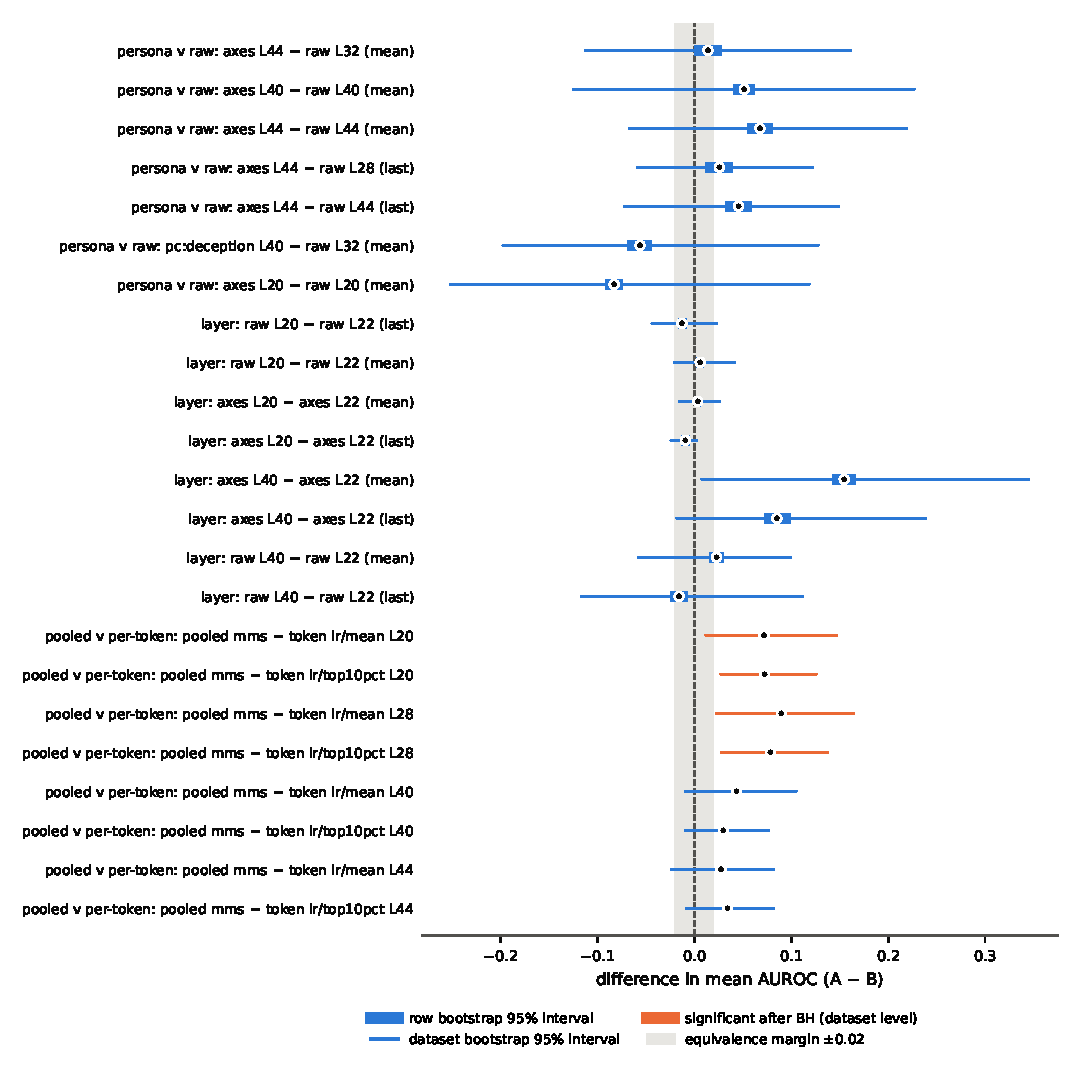
\includegraphics[width=0.92\linewidth]{fig_significance_forest.pdf}
\caption{One test family: each difference with its dataset-bootstrap interval and, where recorded, its row-bootstrap interval.}
\label{fig:r-significance}
\end{figure}
% src: thesis/images/fig_significance_forest.pdf, written by thesis_tools/figures/fig_significance_forest.py from run-coords/significance.json (every plotted value printed by the script; preview thesis_tools/figures/preview/fig_significance_forest.png); the 8 Q8 comparisons have row_ci95 absent (row_p None), so they carry only the dataset interval

\paragraph{Random-direction nulls.}
A zero-shot AUROC has to be compared with random directions, not with 0.5 (Section~\ref{sec:m-controls}).
We scored the paper16 deception contrast (8 v 7) zero-shot at layer 40 with mean pooling on each of the nine labelled datasets, against 1{,}000 random unit directions on the same rows. % src: run-coords/zeroshot_nulls.json :: corpus_L40_mean.per_dataset (9 datasets), n_random 1000; src/assistant_axis_ndif/25_zeroshot_nulls.py :: 81, 94-110 (bank run-paper16/axes_vectors_s3_fp32.pt, axis "deception"); src/assistant_axis_ndif/6_axes.py :: 176 (deception = deception v honesty)
A random direction's sign is arbitrary, so the null is taken over the distance from 0.5, and we quote its 95th percentile as 0.5 plus that distance. % src: src/assistant_axis_ndif/25_zeroshot_nulls.py :: 11-14 (docstring), 63-73 (random_p95_auroc_dev = 95th percentile of |AUROC - 0.5| + 0.5; beats_random_p95 compares |AUROC - 0.5|)
It clears the 95th percentile of its null on five: ai\_liar, IT, ID, roleplaying and sandbagging\_v2. % src: run-coords/zeroshot_nulls.json :: corpus_L40_mean.per_dataset :: beats_random_p95 true for ai_liar, insider-trading, instructed-deception, roleplaying, sandbagging_v2
It lies inside the null on the other four. % src: same :: beats_random_p95 false for convincing-game, harm-pressure-choice, harm-pressure-knowledge-report, mask
On CG it reads 0.7884, which looks like detection against 0.5 but is below the null's 95th percentile of 0.9173 ($p=0.2378$). % src: same :: convincing-game :: auroc 0.78838, random_p95_auroc_dev 0.91728, p_vs_random 0.23776
On HP-KR it reads 0.6436 against a 95th percentile of 0.9377, on HP-C 0.5439 against 0.7732, and on mask 0.4669 against 0.6404. % src: same :: harm-pressure-knowledge-report 0.64358 / 0.93772; harm-pressure-choice 0.54388 / 0.77323; mask 0.46690 / 0.64040
The null's 95th percentile runs from 0.6404 on mask to 0.9477 on IT, so the same AUROC can be strong evidence on one dataset and none on another. % src: same :: random_p95_auroc_dev min 0.64040 (mask), max 0.94773 (insider-trading); interp: the spread of the per-dataset nulls
At layer 44 with last-token pooling (post hoc) the axis clears the null on four of the nine, as sandbagging\_v2 falls inside it (0.8600 against 0.8861). % src: same :: corpus_L44_last.per_dataset :: beats_random_p95 true for ai_liar, IT, ID, roleplaying; sandbagging_v2 auroc 0.86004, p95 0.88610
Pooled over the nine labelled datasets together with the honest Alpaca rows, the axis clears its null at both settings: 0.8810 against a 95th percentile of 0.7636 at layer 40. % src: same :: corpus_L40_mean.pooled :: deception_axis auroc 0.88095, random_p95_auroc_dev 0.76364; corpus_L44_last.pooled :: 0.86512 vs 0.72970; src/assistant_axis_ndif/25_zeroshot_nulls.py :: 101-113 (every run-coords/passB dataset except sycophancy_mt enters the pooled set, including the honest-only Alpaca control; per_dataset keeps only two-class datasets); Alpaca is in passB: lab PC C:/Users/user4/expLB/run-coords/passB/alpaca/ (chunk_0000.pt, 2026-09-15; listed in the lab census audit/phase1/labpc/labpc_census.tsv :: 1937; re-check on the lab PC); the pooled value without single-class datasets is 0.8630 in run-coords/dotproducts_mean.json (12_dotproduct_layers.py, not used here)
Section~\ref{sec:r-cap} gives the same test for the sycophancy contrast, and Section~\ref{sec:r-organisms} for the model organisms.
Pipeline~B has no zero-shot random null; its random control is a trained probe on three random directions, which Section~\ref{sec:r-zeroshot} reports. % src: collaborator persona_ood.py @16def2de :: 61 (N_RANDOM_DRAWS 5), 475 (random_directions), 1062-1065 (random3 matrix, trained); no random-direction null for the one-dimensional arms in persona_ood.py (grep 'null', 2026-09-25)

\paragraph{Response length.}
A detector that sees only the number of response tokens transfers above chance.
In the eleven-dataset store at layer 40 (mean pooling, \texttt{paper} probe), \texttt{length} reaches an off-diagonal mean AUROC of 0.5555 over 110 pairs, against 0.6623 for \texttt{raw}. % src: run-crossgen/kd11/matrices/mean_L40_s42.json :: results[('length','paper')], results[('raw','paper')] :: off-diagonal means 0.55545 / 0.66227 over 110 pairs, computed
The \texttt{length} value is 0.5555 in every matrix of that store, at all 21 layers, both poolings and all three probes, because a probe on one fixed feature can only choose its sign. % src: run-crossgen/kd11/matrices/*.json (42 matrices x 3 probes = 126 cells) :: length off-diagonal mean 0.5555 in all 126, computed 2026-09-25; interp: the reason, from collaborator paper/sections/method.tex @16def2de :: 109-111 (a one-feature probe learns only a sign and a scale)
A random five-direction projection does better, at 0.5849. % src: run-crossgen/kd11/matrices/mean_L40_s42.json :: results[('random','paper')] off-diagonal mean 0.58494
In a separate store at layer 44 (post hoc) with last-token pooling and the \texttt{mms} probe, over the nine labelled datasets and \texttt{sycophancy\_mt} (90 pairs), \texttt{length} reads 0.5533 against 0.6646 for \texttt{raw}. % src: lab PC C:/Users/user4/expLB/run-coords/p1_L44_last_lengthctl.json (cache audit/cache/labpc/run-coords/p1_L44_last_lengthctl.json) :: p1[3] (length, mms) off_diagonal 0.55334; p1[0] (raw, mms) off_diagonal 0.66458; n_pairs 90; matrix sources (10 datasets)
Two different counts describe how response length differs between the classes, and they cover different dataset sets.
By mean response tokens, the deceptive class is longer in 9 of the 11 datasets of the main store; the exceptions are CG ($-1.20$ tokens) and roleplaying ($-4.10$). % src: lab PC C:/Users/user4/expLB/run-coords/passB/<dataset>/rows.jsonl (cache audit/p17/labcache/expLB/run-coords/passB/<dataset>/rows.jsonl) :: mean span_len by label, computed: 9 of 11 positive; convincing-game -1.1976, roleplaying -4.1039
The gap exceeds 40 tokens on only three of them: sandbagging\_v2 ($+189.0$ tokens), mask ($+106.8$) and \texttt{sycophancy\_mt} ($+44.0$); the next largest is ai\_liar, at $+22.4$. % src: same :: sandbagging_v2 +189.0100, mask +106.7596, sycophancy_mt +43.9703, ai_liar +22.3704
On HP-C the responses are about one token long, and the gap is $+0.0035$ tokens. % src: same :: harm-pressure-choice mean span_len 1.0075 (deceptive) and 1.0040 (honest), gap +0.0035
By length-only AUROC within each dataset, length separates the classes above 0.5 on 9 of the 10 datasets of the layer-44 store; roleplaying is the exception, at 0.4415. % src: lab PC C:/Users/user4/expLB/run-coords/confounds_L44_last.json (cache audit/cache/labpc/run-coords/confounds_L44_last.json) :: confounds.length_only_auroc (10 datasets), roleplaying auroc_from_length 0.44147
Two of those nine are barely above chance: CG at 0.5068 and HP-C at 0.5017. % src: same :: convincing-game 0.50677, harm-pressure-choice 0.50173
Transfer numbers in this chapter should therefore be read against 0.5555 for \texttt{length} and 0.5849 for \texttt{random}, not against 0.5. % interp: length 0.5555 and random 0.5849 off-diagonal at layer 40, both above 0.5

\paragraph{Dataset identity.}
The activations record which dataset a row comes from far more strongly than whether the row is a lie. % interp: dataset accuracy 0.9934 against label accuracy 0.6462 (next two lines)
At layer 40 with mean pooling, sampling at most 400 rows per dataset, a standardised logistic regression identifies a row's dataset with three-fold cross-validated accuracy 0.9934. % src: run-coords/validate_L40.json :: dataset_acc 0.99338 (layer 40, pooling mean); src/assistant_axis_ndif/17_validate.py :: 58 (--cap 400), 120-125 (StandardScaler + LogisticRegression C=0.1, cross_val_score cv=3, datasets with at least 100 sampled rows)
The same probe on the same rows predicts the label with accuracy 0.6462. % src: run-coords/validate_L40.json :: label_acc 0.64625
The label's larger class covers 0.614 of the same rows, so the probe gains 0.032 over always guessing it; the largest dataset covers 0.110, so the dataset probe gains 0.883. % src: lab PC C:/Users/user4/expLB/logs/validate.log (cache audit/cache/labpc/logs/validate.log, UTF-16, md5 fc50a5ba3d0cafce9167668e3df4e87d, MANIFEST.csv MATCH 2026-09-25) :: line 22 "label : 0.646 (majority baseline 0.614) lift +0.032"; line 23 "dataset : 0.993 (majority baseline 0.110) lift +0.883 over 10 datasets"; log-only values (run of 2026-09-16 18:45, src/assistant_axis_ndif/17_validate.py), not in run-coords/validate_L40.json
The second and third principal components of these activations each separate one dataset from the rest perfectly (HP-C and IT, AUROC 1.0000), while their AUROCs for the label are 0.4973 and 0.4927. % src: run-coords/validate_L40.json :: pcs[1] (auroc_label 0.49733, best_dataset harm-pressure-choice, auroc_dataset 1.0), pcs[2] (0.49269, insider-trading, 1.0)
The first component, with 25.68\% of the variance, also separates HP-C (AUROC 0.9996), and its label AUROC is 0.2959, which is as far from chance as 0.7041 because a component's sign is arbitrary. % src: run-coords/validate_L40.json :: variance[0] 0.25675, pcs[0] (auroc_label 0.29592, best_dataset harm-pressure-choice, auroc_dataset 0.99962); 1 - 0.29592 = 0.70408
The paper16 deception contrast lies mostly outside the high-variance directions: 16.58\% of its squared norm falls inside the ten leading components. % src: run-coords/validate_L40.json :: deception_in_top10 0.16582; 17_validate.py :: 140 (sum of the squared projections of the unit contrast on the top-10 components)
A \texttt{raw} probe trained on one dataset may fit directions specific to that dataset, which would raise its in-distribution score without helping it elsewhere; a contrast that mostly avoids the high-variance directions has less of that to lose. % interp (not tested directly): dataset accuracy 0.9934 against label accuracy 0.6462; 16.58% of the contrast in the top-10 subspace; the generalisation gaps below

\paragraph{Calibration at the operating point.}
A threshold that flags 1\% of Alpaca need not flag 1\% of another dataset's honest rows (Section~\ref{sec:m-metrics}).
Only Pipeline~B records specificity, so only its detections can be checked. % src: collaborator results/persona_ood_ext_L*/zero_shot_operating.csv @16def2de :: column specificity; src/assistant_axis_ndif/27_crossgen.py :: 275-279 (Pipeline A records TPR only)
Over the six arms (the base probe and the five zero-shot contrasts), the five Liars' Bench datasets and layers 20, 40 and 44 (44 post hoc), 24 of the 90 cells run above a 1\% realised false-positive rate. % src: collaborator results/persona_ood_ext_L{20,40,44}/zero_shot_operating.csv @16def2de :: threshold_source 'control', RepE rows excluded, 1 - specificity > 0.01 in 24 of 90 rows, computed 2026-09-25
Seventeen of the 24 are on ID, where every arm exceeds 1\% at layers 40 and 44 and the base probe reaches 15.21\% at layer 40. % src: same :: instruct_dishonesty__plain rows (17 of 24); layer 40 base probe (RepE-trained) specificity 0.8479
The others are three cells of the denial contrast (4 v 6) on HP-KR, three on IT and one on HP-C; the worst, on HP-KR at layer 20, is discussed in Section~\ref{sec:r-hpkr}. % src: same :: harm_refusal_knowledge_report (4v6 at L20, L40, L44), insider_trading_cadenza (base L20, 8v7 L40, 12v13 L40), harm_refusal_choice (4v6 L20)
Across all 16 layers of Pipeline~B's sweep, 122 of the 480 such cells exceed 1\%. % src: collaborator results/persona_ood_ext_L{20,24,...,76,79}/zero_shot_operating.csv @16def2de :: same rule, 16 layers x 6 arms x 5 datasets, computed
Table~\ref{tab:r-oracle} separates the direction from the threshold by re-scoring each detector with the oracle threshold of Section~\ref{sec:r-testing}, which is set at 1\% false positives on each dataset's own honest rows and therefore uses the labels. % src: collaborator deception_detection/scripts/persona_ood.py @16def2de :: 579-583 (control v in-dataset (oracle) definitions), 613-620 (oracle threshold = the 0.99 quantile of the dataset's own honest scores)
At layer 40 the oracle threshold lowers the denial contrast's Liars' Bench average balanced accuracy from 0.7251 to 0.6921, and raises the extended contrast's from 0.6939 to 0.7183 and the base probe's from 0.6255 to 0.6519. % src: collaborator results/persona_ood_ext_L40/zero_shot_operating.csv @16def2de :: dataset "Average (Liars' Bench)", balacc, threshold_source control v "in-dataset (oracle)"
Part of the denial contrast's lead under the Alpaca threshold therefore comes from running above 1\% false positives on some datasets, and under the oracle threshold the extended contrast leads. % interp: 0.7251 -> 0.6921 (D8) against 0.6939 -> 0.7183 (D9); D8's realised false-positive rate on ID at layer 40 is 11.86% (specificity 0.8814, same file)
Under either threshold both contrasts stay above the base probe at layer 40, and under the Alpaca threshold the denial contrast's interval, $[0.7154, 0.7348]$, lies clear of the base probe's, $[0.6185, 0.6330]$. % src: same :: balacc_lo / balacc_hi of the Liars' Bench average rows
At layer 36 (post hoc) the oracle threshold lowers all three detectors, and the extended contrast leads under both thresholds. % src: collaborator results/persona_ood_ext_L36/zero_shot_operating.csv @16def2de :: "Average (Liars' Bench)" balacc, control v oracle
The intervals in the table are Pipeline~B's row-level intervals from one model. % src: collaborator paper/sections/setup.tex @16def2de :: 39-40; collaborator deception_detection/scripts/persona_ood.py @16def2de :: 570-574

\begin{table}[t]
\centering
\footnotesize
\caption{Liars' Bench average balanced accuracy at the Alpaca threshold and at the oracle threshold (Pipeline~B).}
\label{tab:r-oracle}
\begin{tabular}{lll}
\hline
Design and layer & Alpaca threshold & Oracle threshold \\
\hline
\multicolumn{3}{l}{\emph{L36 (post hoc)}} \\
D2 base probe & 0.6500 [0.6416, 0.6583] & 0.6347 [0.6228, 0.6460] \\
D8 knowledge-denial contrast (4 v 6) & 0.6948 [0.6841, 0.7047] & 0.6747 [0.6612, 0.6874] \\
D9 extended contrast (12 v 13) & 0.7115 [0.7029, 0.7198] & 0.7099 [0.6975, 0.7215] \\
\multicolumn{3}{l}{\emph{L40}} \\
D2 base probe & 0.6255 [0.6185, 0.6330] & 0.6519 [0.6400, 0.6625] \\
D8 knowledge-denial contrast (4 v 6) & 0.7251 [0.7154, 0.7348] & 0.6921 [0.6799, 0.7054] \\
D9 extended contrast (12 v 13) & 0.6939 [0.6855, 0.7023] & 0.7183 [0.7060, 0.7306] \\
\hline
\end{tabular}
\end{table}
% src: collaborator results/persona_ood_ext_L36/zero_shot_operating.csv @16def2de :: dataset "Average (Liars' Bench)", arms 'base probe (RepE-trained)', 'knowledge-denial axis (4v6)', 'extended axis (12v13)'; columns balacc [balacc_lo, balacc_hi]; threshold_source control (Alpaca) and "in-dataset (oracle)" -- file rows 89/97, 57/65, 41/49
% src: collaborator results/persona_ood_ext_L40/zero_shot_operating.csv @16def2de :: same rows and columns -- file rows 89/97, 57/65, 41/49
% note: intervals are 95% stratified bootstrap intervals over examples, 1,000 resamples (persona_ood.py :: 564, 572-574)

\paragraph{The generalisation gap.}
The generalisation gap of Section~\ref{sec:r-criteria} measures how much of its in-distribution score a detector loses on other datasets.
In Pipeline~B (six datasets), the single-source \texttt{raw} probe (D1, \texttt{lr\_reg10}) has an in-distribution AUROC between 0.9564 and 0.9838 across the 16 layers, and loses between 0.2130 (layer 36, post hoc) and 0.3469 (layer 24) off-diagonal. % src: collaborator results/persona_ood_ext_L{20,24,...,76,79}/summary.csv @16def2de :: row baseline :: diagonal_mean (min 0.95641 at L20, max 0.98376 at L52); diagonal_mean - off_diagonal_mean (min 0.21301 at L36, max 0.34685 at L24), computed; six datasets: collaborator paper/sections/setup.tex @16def2de :: 21-23
Section~\ref{sec:r-problem} gives its values at layer 40.
In Pipeline~A, the \texttt{raw} probe (mean pooling, \texttt{paper} probe, eleven datasets) loses 0.2979 at layer 40, and between 0.2795 (layer 32) and 0.3270 (layer 22) across the layers from 20 up. % src: run-crossgen/kd11/summary.json :: records[feature raw, probe paper, pooling mean, seed 42].generalization_gap_10 :: L40 0.29794; min over L>=20 0.27950 (L32), max 0.32698 (L22)
The two pipelines measure the in-distribution score differently, by five-fold cross-validation on the whole source in Pipeline~B and on an 80/20 split by item in Pipeline~A, so we do not compare their gaps directly. % src: Chapter 4, Section sec:m-protocols (collaborator paper/sections/setup.tex @16def2de :: 21-29; src/assistant_axis_ndif/27_crossgen.py :: 194-217)
The extended contrast (D9) shows no gap: at each of the 16 layers its off-diagonal mean is within 0.0018 of its in-distribution score. % src: collaborator results/persona_ood_ext_L*/summary.csv @16def2de :: row ext_axis1 :: diagonal_mean - off_diagonal_mean in [-0.00172 (L60), +0.00002 (L48)], computed
The knowledge-denial contrast (D8) is within 0.0060. % src: same :: row denial_axis1 :: diagonal_mean - off_diagonal_mean in [-0.00594 (L68), -0.00010 (L32)], computed
This holds by construction and is not evidence that the contrasts generalise better: a one-dimensional score can learn only a sign and a scale, so it has no training set to overfit and nothing to lose off-diagonal (Section~\ref{sec:m-protocols}). % src: collaborator paper/sections/method.tex @16def2de :: 109-112; interp: the near-zero gaps of D8 and D9 follow from this
The informative comparison for the contrasts is their off-diagonal level, which Section~\ref{sec:r-transfer} reports. % interp

% ===== PART W6b (verified) =====
% =====================================================================
% Chapter 5, Section 5.5 -- Comparisons and Relationships (part W6b)
% Plan: thesis_tools/planning/CH5_RESULTS_PLAN.md, section 5.5.
% Collaborator files are read at the pin (git show 16def2de:<path>). Lab-PC values come from the
% local caches audit/cache/labpc/ and audit/p17/labcache/, and are re-checked on the lab PC in the
% final verification session. Every value below was re-read or recomputed from those files on 2026-09-25.
% =====================================================================

% ---------------------------------------------------------------------
\section{Comparisons and Relationships}
\label{sec:r-compare}

This section sets our results beside four references: the benchmark's own probes and protocol, the persona-coordinate method we replicated, the same pipeline on smaller models, and supervised probes trained on many datasets at once.
It ends by relating the geometry of the contrast directions to how they behave as detectors.
Each comparison names the pipeline that produced it.
Where both pipelines measured the same quantity we report both, in separate sentences, because Pipeline~B trains a single-source probe on all of its source's rows and Pipeline~A on a class-balanced 80\% split (Section~\ref{sec:m-protocols}). % src: collaborator deception_detection/scripts/persona_ood.py @16def2de :: 301-303 (probe.fit on the whole training dataset); src/assistant_axis_ndif/27_crossgen.py :: 881 (--frac 0.8); src/assistant_axis_ndif/9_persona_probes.py :: 263-274 (balance)

\subsection{With the benchmark's probes and protocol}
\label{sec:r-cmp-lb}

Liars' Bench scores a detector by its balanced accuracy at a threshold that flags at most 1\% of the Alpaca control, and reports AUROC and recall (the true-positive rate) at the same threshold as secondary metrics \parencite[p.~7]{kretschmar2025liars}.
Only Pipeline~B records balanced accuracy and specificity; Pipeline~A records the true-positive rate alone (Section~\ref{sec:m-metrics}), so this comparison uses Pipeline~B. % src: collaborator persona_ood.py @16def2de :: 203-217 (balanced_accuracy, specificity); src/assistant_axis_ndif/9_persona_probes.py :: 238-243 (tpr_at_fpr only)
Table~\ref{tab:r-protocol} sets three zero-shot contrasts on the knowledge-denial bank beside the base probe under that protocol, on mean-pooled response activations, averaged over the five Liars' Bench datasets, at layers 20, 40 and 44 (post hoc). % src: collaborator results/persona_ood_ext_L{20,40,44}/zero_shot_operating.csv @16def2de :: rows dataset = "Average (Liars' Bench)", threshold_source = control (n_deceptive 3908 = 167 + 134 + 139 + 423 + 3045, the five non-RepE datasets); collaborator paper/sections/method.tex @16def2de :: 121 ("We mean-pool them into one vector")

\begin{table}[t]
\centering
\footnotesize
\caption{Detection under the Liars' Bench protocol, averaged over its five datasets (Pipeline~B).}
\label{tab:r-protocol}
\begin{tabular}{llrrr}
\hline
Layer & Detector & Balanced acc. & Recall & AUROC \\
\hline
L20 & base probe (trained on RepE) & \textbf{0.7209} & \textbf{0.4893} & 0.6972 \\
 & published contrast (8 v 7), zero-shot & 0.5342 & 0.0692 & 0.7503 \\
 & knowledge-denial contrast (4 v 6), zero-shot & 0.5587 & 0.3053 & 0.8628 \\
 & extended contrast (12 v 13), zero-shot & 0.5914 & 0.1872 & \textbf{0.8868} \\
\hline
L40 & base probe (trained on RepE) & 0.6255 & 0.2814 & 0.7784 \\
 & published contrast (8 v 7), zero-shot & 0.675 & 0.3819 & 0.7983 \\
 & knowledge-denial contrast (4 v 6), zero-shot & \textbf{0.7251} & \textbf{0.4868} & 0.8938 \\
 & extended contrast (12 v 13), zero-shot & 0.6939 & 0.4129 & \textbf{0.899} \\
\hline
L44 (post hoc) & base probe (trained on RepE) & 0.6256 & 0.2812 & 0.7564 \\
 & published contrast (8 v 7), zero-shot & 0.6535 & 0.318 & 0.7913 \\
 & knowledge-denial contrast (4 v 6), zero-shot & \textbf{0.6829} & \textbf{0.3949} & 0.8802 \\
 & extended contrast (12 v 13), zero-shot & 0.6663 & 0.3503 & \textbf{0.8841} \\
\hline
\end{tabular}
\end{table}
% src: collaborator results/persona_ood_ext_L20/zero_shot_operating.csv @16def2de :: dataset "Average (Liars' Bench)", threshold_source control, columns balacc / recall / auroc; arms "base probe (RepE-trained)" 0.7209/0.4893/0.6972, "deception axis (8v7)" 0.5342/0.0692/0.7503, "knowledge-denial axis (4v6)" 0.5587/0.3053/0.8628, "extended axis (12v13)" 0.5914/0.1872/0.8868
% src: collaborator results/persona_ood_ext_L40/zero_shot_operating.csv @16def2de :: same rows; base 0.6255/0.2814/0.7784; 8v7 0.675/0.3819/0.7983; 4v6 0.7251/0.4868/0.8938; 12v13 0.6939/0.4129/0.899
% src: collaborator results/persona_ood_ext_L44/zero_shot_operating.csv @16def2de :: same rows; base 0.6256/0.2812/0.7564; 8v7 0.6535/0.318/0.7913; 4v6 0.6829/0.3949/0.8802; 12v13 0.6663/0.3503/0.8841
% note: values copied at the CSV's own precision (0.675, 0.899 and 0.318 are stored with three decimals); bold = best in each layer block. Pipeline B's own rendering is paper/generated/tab_operating.tex @16def2de (3 decimals).

At layer 40 the knowledge-denial contrast (4 v 6) is the best detector at the threshold, with balanced accuracy 0.7251 and recall 0.4868, while the extended contrast (12 v 13) ranks best, with AUROC 0.899. % src: collaborator results/persona_ood_ext_L40/zero_shot_operating.csv @16def2de :: "Average (Liars' Bench)", control; 4v6 balacc 0.7251, recall 0.4868; 12v13 auroc 0.899
The base probe reaches 0.6255, 0.2814 and 0.7784 on the same three metrics. % src: same file :: arm "base probe (RepE-trained)", balacc 0.6255, recall 0.2814, auroc 0.7784
At layers 40 and 44, each of the three contrasts beats the base probe on all three metrics. % src: persona_ood_ext_L40 and _L44/zero_shot_operating.csv @16def2de :: "Average (Liars' Bench)", control; every contrast's balacc, recall and auroc above the base probe's (Table rows above)
At layer 20 the order reverses at the threshold: the base probe leads on balanced accuracy (0.7209) and recall (0.4893), and has the lowest AUROC of the four (0.6972). % src: collaborator results/persona_ood_ext_L20/zero_shot_operating.csv @16def2de :: "Average (Liars' Bench)", control; base 0.7209 / 0.4893 / 0.6972 against 8v7 0.7503, 4v6 0.8628, 12v13 0.8868 AUROC

Part of that lead is real detection.
On CG at layer 20 the base probe's recall is 0.6766 against 0.1737 for the extended contrast, and both have specificity 1.0 there. % src: collaborator results/persona_ood_ext_L20/zero_shot_operating.csv @16def2de :: dataset convince_me__plain, control; base recall 0.6766 specificity 1.0; 12v13 recall 0.1737 specificity 1.0
Part of it comes from false positives: the Alpaca threshold leaves the base probe a specificity of 0.8691 on IT and 0.8936 on ID, against 1.0 and 0.9778 for the extended contrast, which ranks both datasets at least as well (AUROC 0.9899 and 0.9539, against 0.9726 and 0.9498). % src: same file :: insider_trading_cadenza__plain and instruct_dishonesty__plain, control; base specificity 0.8691 / 0.8936, auroc 0.9726 / 0.9498; 12v13 specificity 1.0 / 0.9778, auroc 0.9899 / 0.9539
% interp: at layer 20 the base probe's lead at the threshold is partly bought with realised false-positive rates far above 1% on IT and ID (1 - 0.8691, 1 - 0.8936), while on ranking the extended contrast is ahead on both.
Section~\ref{sec:r-stats} gives the realised false-positive rate of every cell.

Figure~\ref{fig:r-operating} breaks the layer-40 average down by dataset.
Three features stand out.
First, HP-C defeats every detector at the threshold: the base probe, the published contrast and the extended contrast all have balanced accuracy 0.5 on it, and the knowledge-denial contrast 0.5075. % src: collaborator results/persona_ood_ext_L40/zero_shot_operating.csv @16def2de :: harm_refusal_choice__plain, control, balacc (base 0.5, 8v7 0.5, 12v13 0.5, 4v6 0.5075)
Second, the knowledge-denial contrast ranks IT well (AUROC 0.9134) but flags none of its lies (recall 0.0), while the published and extended contrasts flag 0.8723 and 0.7494 of them. % src: same file :: insider_trading_cadenza__plain, control; 4v6 auroc 0.9134 recall 0.0; 8v7 recall 0.8723; 12v13 recall 0.7494
Third, the base probe ranks IT backwards at layer 40, with AUROC 0.3378. % src: same file :: insider_trading_cadenza__plain, base probe (RepE-trained), auroc 0.3378
% interp: no single arm wins every dataset at the threshold; against the extended contrast, the knowledge-denial contrast's average lead (0.7251 vs 0.6939) comes from HP-KR (0.9102 vs 0.5) and CG (0.7784 vs 0.6796) and is partly given back on IT (0.5 vs 0.8686), per the L40 per-dataset balacc rows.
HP-KR, where only the knowledge-denial contrast flags lies, is treated in Section~\ref{sec:r-hpkr}, and the benchmark's published probe scores in Section~\ref{sec:r-problem}.

\begin{figure}[t]
\centering
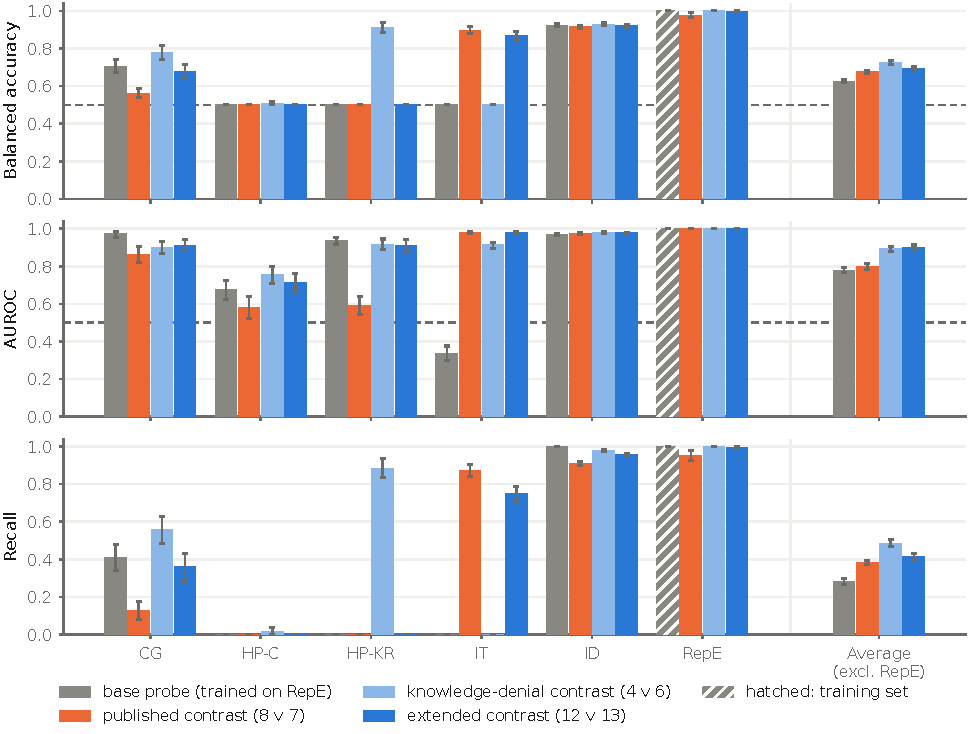
\includegraphics[width=\linewidth]{collab_fig_operating.pdf}
\caption{Per-dataset detection at layer 40 under the Liars' Bench protocol, produced by Pipeline~B.}
\label{fig:r-operating}
\end{figure}
% src: thesis/images/collab_fig_operating.pdf = git cat-file blob 16def2deec34aeee532511df116adb7de5522ca7:src/probes/deception-detection/paper/generated/fig_operating.pdf (blob 0248b80a; 25,704 bytes, equal to git cat-file -s; md5 4e3397c176f663084d6a805f26d5d63b); drawn by paper/make_figures.py :: operating() (layer 40, threshold_source control, panels balanced accuracy / AUROC / recall, bars = base probe, 8v7, 4v6, 12v13; RepE hatched for the base probe, whose training set it is; the average excludes RepE)

One setting differs from the benchmark's.
Pipeline~B's insider-trading scores exclude the model's reasoning scratchpad (Section~\ref{sec:m-data}), whereas the benchmark's Mean Probe reads it \parencite[p.~8]{kretschmar2025liars}. % src: collaborator paper/sections/method.tex @16def2de :: 126-127
In the benchmark's own ablation on Llama-3.3-70B at layer 20, excluding the scratchpad raises the Mean Probe's insider-trading AUROC from 0.93 to 0.97 \parencite[p.~70]{kretschmar2025liars}. % src: papers/2511.16035v2 (1).pdf :: PDF p. 70, Table 17, row "Layer 20", AUROC w/ Reas. 0.93, w/o Reas. 0.97 (read 2026-09-25); same pair in collaborator paper/generated/numbers.tex @16def2de :: 1075-1076 (lb-it-reas-auroc 0.93, lb-it-noreas-auroc 0.97)
The benchmark also averages each published score over several models before averaging over datasets \parencite[p.~7]{kretschmar2025liars}, whereas Pipeline~B's averages cover Llama-3.3-70B-Instruct alone. % src: papers/2511.16035v2 (1).pdf :: PDF p. 7 ("we first calculate it for every model/dataset pair, then average over models, and finally datasets"); collaborator paper/sections/method.tex @16def2de :: 116 (Llama-3.3-70B-Instruct)
Comparisons between Pipeline~B's numbers and the benchmark's published ones, on IT above all, are therefore approximate.

\subsection{With the replicated method at 70B}
\label{sec:r-cmp-replication}

\textcite[p.~4]{mahadik2026persona} built their persona coordinates on Llama~3.2-3B and replicated their findings on Llama~3-8B. % src: papers/Do Linear Probes Generalize Better in Persona Coordinates.pdf :: PDF p. 4 ("Our main results use Llama 3.2-3B, with additional replications on Llama 3-8B"; "The following findings are replicated with a larger 8B model")
On those models, probes trained on the top three persona components transferred better than probes on raw activations for most train--test pairs \parencite[p.~4]{mahadik2026persona}. % src: same PDF :: p. 4 ("Projecting dataset activations onto the top 3 PCs of the persona axis and training probes on those projected features improves cross-dataset generalization for most train-test pairs")
They describe the 8B results as broadly supportive and name larger scales as untested \parencite[p.~5]{mahadik2026persona}. % src: same PDF :: p. 5 ("The auxiliary 8B comparisons in Appendix F are broadly supportive"; "Our findings need to be replicated across more model families and larger scales")
They also report that the unified-axis features gain most where raw probes transfer poorly \parencite[p.~4]{mahadik2026persona}. % src: same PDF :: p. 4 ("The unified-axis projection gives its largest gains where raw probes transfer poorly")
Their figures evaluate five deception datasets: CG, ID, MASK, ai\_liar and roleplaying \parencite[p.~6]{mahadik2026persona}. % src: same PDF :: p. 6, Figure 4 axes (ConvGame, InstrDec, Mask, AILiar, Roleplay); note: Table 1 on p. 4 lists HarmPressureChoice where the figures use Mask

Pipeline~A tested the method at 70B in five ways.
\begin{itemize}
\item \textbf{Like for like.} On the paper16 bank and those five datasets, with three components, mean pooling and the \texttt{paper} probe, we took at each layer the better of \texttt{axes} and \texttt{pc:deception} (a choice made after seeing the results). % src: lab PC C:/Users/user4/expLB/run-crossgen/scale_70b_paper16fp32/matrices/mean_L*_s42.json (cache audit/p17/labcache/expLB/run-crossgen/scale_70b_paper16fp32/matrices/) :: bank_name paper16_70b_fp32, k 3, datasets [instructed-deception, mask, convincing-game, ai_liar, roleplaying], results[feature, probe=paper].auroc
Averaged over the 19 layers from 0 to 68, it trails \texttt{raw} by 0.0131 in mean off-diagonal AUROC and leads \texttt{datapca} by 0.0541. % src: same files, L0-L68 (19 layers) :: off-diagonal mean over the 20 train != test pairs; mean over layers of max(axes, pc:deception) - raw = -0.0131, - datapca = +0.0541 (recomputed 2026-09-25; reproduces audit/fix/rf16_recompute_mean.txt's recipe)
Over all 21 stored layers the two margins are $-0.0171$ and $+0.0550$. % src: same files, all 21 layers (L0-L76) :: -0.0171 / +0.0550
This is one seed with no dataset bootstrap. % src: same files :: seed 42 only
% interp: at 70B the persona components beat a matched low-dimensional control but not the raw probe, whichever layer set is averaged.
\item \textbf{Against the matched control.} On our datasets, the unified components, which the paper reports gaining most where raw probes transfer poorly, lose their advantage once they are matched against \texttt{datapca} at the same $k$ (Section~\ref{sec:r-stats}). % src: run-crossgen/significance.json :: block 10, pooling mean, layer 40, probe paper, comparison "pc:unified@2 - datapca@2" (diff -0.0028, dataset_p 0.9632; identical in audit/cache/labpc/run-crossgen/significance.json); the number is reported in Section 5.4
\item \textbf{Across layers.} The layer sweep, at $k=5$ on the paper16 bank, finds \texttt{pc:deception} below \texttt{raw} at every layer from 20 upwards in all four of its runs: \texttt{lr\_reg10} and \texttt{mms} under mean pooling, \texttt{mms} under mean pooling again in a second activation store, and \texttt{mms} under last-token pooling (Section~\ref{sec:r-layer}). % src: run-coords/layer_sweep_mean.json (lr_reg10, mean), layer_sweep_mms.json (mms, mean), layer_sweep_passB_mms.json (mms, mean, passB store), layer_sweep_passB_last.json (mms, last) :: k 5, bank axes_vectors_s3_fp32.pt; sweep[*]["pc:deception"] < sweep[*]["raw"] at every layer >= 20; above raw only at L0 (lr_reg10, mean) and at L0, L8, L16 (mms, last)
\item \textbf{On our datasets.} On the ten-dataset grid at layer 40 (mean pooling, \texttt{paper} probe), \texttt{pc:unified@2} trails \texttt{raw} by 0.0338 in mean off-diagonal AUROC, and leads it by 0.0281 on the nine datasets without \texttt{sycophancy\_mt}. % src: run-crossgen/summary.json :: records[pooling mean, layer 40, seed 42, probe paper]; pc:unified@2 offdiag_mean_10 0.6314 vs raw 0.6652 (-0.0338); offdiag_mean_9 0.7187 vs raw 0.6906 (+0.0281); identical in audit/cache/labpc/run-crossgen/summary.json
\texttt{pc:deception} reads $-0.0268$ and $+0.0276$ on the same two sets. % src: same :: pc:deception offdiag_mean_10 0.6384 (-0.0268), offdiag_mean_9 0.7181 (+0.0276)
None of the four differences clears the dataset bootstrap ($P$ from 0.665 to 0.7938). % src: run-crossgen/significance.json :: block 10 / block 9, mean, L40, paper; "pc:deception - raw" dataset_p 0.665 / 0.6758; "pc:unified@2 - raw" dataset_p 0.7 / 0.7938
The unified components of this bank follow its question sets rather than its roles (Section~\ref{sec:r-personas}), so the unified row is confounded.
\item \textbf{Around layer 40.} A fine sweep over layers 37--39 and 41--47 on four banks (two builds of paper16, own100 and hf275 under the strict labels of Section~\ref{sec:r-personas}) finds \texttt{axes} below \texttt{raw} in 36 of the 40 (bank, layer) cells, over the ten datasets of the main grid other than the text-matched slice, with mean pooling and the \texttt{paper} probe. % src: lab PC C:/Users/user4/expLB/run-crossgen/passB_fine/summary.json and banks/{hf275_strict,own100,paper16_shared}/summary.json (cache audit/p17/labcache/expLB/run-crossgen/passB_fine/) :: records[pooling mean, probe paper, seed 42], offdiag_mean_10, axes - raw < 0 in 36/40 (exceptions own100 L37 +0.0097, L39 +0.019, L44 +0.0052; paper16_shared L44 +0.0138)
Without \texttt{sycophancy\_mt} the count reverses: \texttt{axes} is ahead in 29 of the 40 cells. % src: same :: offdiag_mean_9, axes - raw < 0 in 11/40, > 0 in 29/40
This sweep is one seed with no dataset bootstrap. % src: same :: seeds [42]
\end{itemize}

Pipeline~B compared its single contrast directions with their own leading components (Section~\ref{sec:r-d4}).
Over all six of its datasets, the zero-shot extended contrast transfers better than a probe trained on its first three components (mean off-diagonal AUROC, mean pooling, the \texttt{lr\_reg10} estimator) at 13 of the 16 swept layers, and falls below it at layers 64, 68 and 72. % src: collaborator results/persona_ood_ext_L{20,...,79}/summary.csv @16def2de :: off_diagonal_mean, ext_axis1 - ext_pc3 > 0 at 13/16 layers; L64 -0.0010, L68 -0.0205, L72 -0.0146; arms ext_axis1 (dim 1, zero-shot) and ext_pc3 (dim 3, trained) per results/loo_L40/loo_summary.csv @16def2de; estimator collaborator persona_ood.py @16def2de :: 190-194 (make_probe: StandardScaler + LogisticRegression C = 1/10, no intercept)
Without HP-KR the count falls to 11 of 16 (Section~\ref{sec:r-d4}), and at layer 20 the contrast's lead shrinks from $+0.2204$ to $+0.0086$. % src: same files :: off_diagonal_excl_hpkr, ext_axis1 - ext_pc3 > 0 at 11/16; L20 off_diagonal_mean +0.2204, off_diagonal_excl_hpkr +0.0086
% interp: Pipeline B's "one direction beats the components at 13 of 16 layers" holds as stated, but much of it is carried by HP-KR, the dataset whose failure motivated the knowledge-denial roles.
In Pipeline~A, then, the paper's own features on the paper16 bank do not transfer better than raw activations at 70B once \texttt{sycophancy\_mt} is in the set, and their gains on the nine deception datasets do not clear the dataset bootstrap; the paper reports the opposite at 3B and 8B. % interp: like-for-like -0.0131 vs raw; ten-dataset retrain -0.0338 (pc:unified@2) and -0.0268 (pc:deception); nine-dataset +0.0281 / +0.0276 with dataset_p 0.7938 / 0.6758; passB_fine 36/40 below raw with sycophancy_mt. Trained components on the kd bank are a different case (Section 5.2.5).

\subsection{Across model scale}
\label{sec:r-scale}

The 3B and 8B rungs (Section~\ref{sec:m-banks}) test whether the 70B result is a property of model size.
All three rungs run Pipeline~A's train-one-test-all grid on the five deception datasets the paper evaluates, none of which holds harm-pressure data, with $k=3$, mean pooling, the \texttt{paper} probe and seed 42. % src: matrices meta in audit/p17/labcache/expLB/run-crossgen/scale_{3b,8b,70b_paper16fp32}/matrices/mean_L*_s42.json and audit/p17/labcache/expLB-resplit/run-crossgen/kdscale_*/matrices/mean_L*_s42.json :: datasets (5), k 3, pooling mean, seed 42
For each layer we take the \emph{best persona feature}, the one with the highest mean off-diagonal AUROC among \texttt{axes}, \texttt{pc:deception}, \texttt{pc:unified} and \texttt{pc:unified@2}, a choice made after seeing the results. % src: audit/scripts/p12_kd_scale_ladder.py :: 59-73 (best = max over pc:* and axes); thesis_tools/figures/fig_scale_ladder.py :: ladder_cell
We subtract \texttt{raw} and average over the layers each rung stores: 7 at 3B, 8 at 8B and 21 at 70B. % src: audit/scripts/p12_kd_scale_ladder.py :: 59-73 (best = max over pc:* and axes, layer-averaged), re-implemented in thesis_tools/figures/fig_scale_ladder.py; layers from the matrix files (3B L0-L24, 8B L0-L28, 70B 21 layers)
Figure~\ref{fig:r-scale} shows the result.

For paper16 the margin falls from $+0.0382$ at 3B to $+0.0148$ at 8B and $-0.0116$ at 70B. % src: lab PC C:/Users/user4/expLB/run-crossgen/scale_{3b,8b,70b_paper16fp32}/matrices/mean_L*_s42.json (cache audit/p17/labcache/expLB/run-crossgen/...) :: layer mean of (best persona feature - raw), probe paper; printed by thesis_tools/figures/fig_scale_ladder.py: +0.0382 / +0.0148 / -0.0116
% note: the 70B paper16 point (-0.0116) and the like-for-like -0.0131 of Section 5.5.2 come from the same matrices; they differ only in the feature set (four persona features here, axes and pc:deception there) and the layer set (21 layers here, L0-L68 there).
For the kd bank at scores 2--3 it falls from $+0.0360$ to $+0.0194$, and at 70B it is barely above zero. % src: lab PC C:/Users/user4/expLB-resplit/run-crossgen/kdscale_{3b,8b,70b}_s23/matrices/mean_L*_s42.json (cache audit/p17/labcache/expLB-resplit/run-crossgen/kdscale_*_s23/) :: +0.0360 / +0.0194 / +0.0054 (the 70B value given as a direction only)
The kd bank with every judge score kept follows the same path: $+0.0317$ and $+0.0169$ at 3B and 8B, and barely above zero at 70B. % src: lab PC C:/Users/user4/expLB-resplit/run-crossgen/kdscale_{3b,8b,70b}_all/matrices/mean_L*_s42.json (cache audit/p17/labcache/expLB-resplit/run-crossgen/kdscale_*_all/matrices/) :: layer mean of (best persona feature - raw) = +0.0317 / +0.0169 / +0.0032 (printed by fig_scale_ladder.py)
Both banks decline, so the decline belongs to the method, not to the bank. % interp: paper16 +0.0382 -> +0.0148 -> -0.0116; kd s23 +0.0360 -> +0.0194 -> +0.0054
The kd bank declines less, so the gap between the two banks moves in its favour as the model grows, but at 70B its best persona feature is only a whisker above \texttt{raw}. % interp: kd s23 minus paper16 = -0.0022 / +0.0046 / +0.0170 (printed by fig_scale_ladder.py); direction only, per the owner's rule for the 70B kd value

The paper's own feature, drawn dashed in Figure~\ref{fig:r-scale}, declines more steeply.
On paper16, \texttt{pc:deception} goes from $+0.0324$ over \texttt{raw} at 3B to $+0.0069$ at 8B and $-0.0321$ at 70B, and it is ahead of \texttt{raw} at 7 of 7, 5 of 8 and 5 of 21 layers. % src: scale_{3b,8b,70b_paper16fp32} matrices (caches above) :: layer mean of pc:deception - raw = +0.0324 / +0.0069 / -0.0321; per-layer pc:deception - raw > 0 at 7/7, 5/8, 5/21 (recomputed 2026-09-25; printed by fig_scale_ladder.py)
At 3B, then, our rebuild agrees in direction with what the paper reports for that size \parencite[p.~4]{mahadik2026persona}, and the agreement fades as the model grows. % interp: pc:deception - raw +0.0324 at 3B (7/7 layers ahead) -> +0.0069 (5/8) -> -0.0321 (5/21); the datasets match the paper's evaluated five, but the layers, splits and bank prompts differ from the paper's
Against \texttt{datapca} at $k=3$, the best persona feature on paper16 stays ahead but by less at each size: $+0.1251$, $+0.1086$ and $+0.0605$. % src: same matrices :: layer mean of (best persona feature - datapca) = +0.1251 / +0.1086 / +0.0605 (printed by fig_scale_ladder.py)
That steady decline is a mean-pooling result. % src: the kdscale_* stores hold only mean_L* matrices (fig_scale_ladder.py prints 0 last_L* files for every kd rung)
With last-token pooling, which only the paper16 rungs store, the margins over \texttt{datapca} are $+0.0964$, $+0.0436$ and $+0.0712$, and those over \texttt{raw} are $+0.0041$, $-0.0396$ and $+0.0100$; neither declines steadily. % src: lab PC C:/Users/user4/expLB/run-crossgen/scale_{3b,8b,70b_paper16fp32}/matrices/last_L*_s42.json (caches audit/p17/labcache/expLB/run-crossgen/...) :: layer mean of (best persona feature - datapca) and (best - raw), probe paper; printed by thesis_tools/figures/fig_scale_ladder.py under 'last-token pooling, paper16'

\begin{figure}[t]
\centering
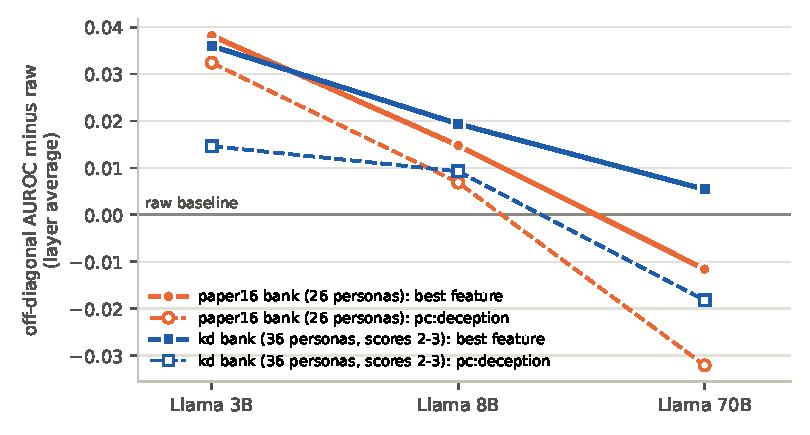
\includegraphics[width=0.78\linewidth]{fig_scale_ladder.pdf}
\caption{Layer-averaged margin of persona features over raw by model size, for two banks (Pipeline~A).}
\label{fig:r-scale}
\end{figure}
% src: thesis/images/fig_scale_ladder.pdf <- thesis_tools/figures/fig_scale_ladder.py (reads audit/p17/labcache/expLB/run-crossgen/scale_* and audit/p17/labcache/expLB-resplit/run-crossgen/kdscale_*_s23; solid = best persona feature - raw, dashed = pc:deception - raw; prints every plotted value); preview thesis_tools/figures/preview/fig_scale_ladder.png

The ladder carries several caveats.
It covers five datasets and none with harm-pressure data, so the kind of lie the kd roles were built for is absent from it. % src: matrices :: datasets [instructed-deception, mask, convincing-game, ai_liar, roleplaying]
It uses $k=3$, one seed and a best feature chosen after the results, and it has no significance test. % src: matrices :: k 3, seed 42; best = post-hoc per-layer max (fig_scale_ladder.py)
The 3B and 8B inputs are cut at 1{,}024 tokens against 8{,}192 at 70B (Section~\ref{sec:m-transform}), so only margins within a rung are compared, never absolute AUROCs across rungs. % src: scale/scripts/run_scale_coords.ps1 :: 117-122 (maxlen 1024; "absolute AUROCs are NOT comparable across model size"); src/assistant_axis_ndif/run_coords_chain.ps1 :: 95 (--max_length 8192)
The 3B and 8B rungs also sample at most 800 rows per dataset, which cuts only ID: its class-balanced training set is 612 rows there against 3{,}808 at 70B, while the other four datasets have the same training rows at every rung. % src: scale/scripts/run_scale_coords.ps1 :: 53-57, 143 (--sample 800, stratified; "three of the five are already under 800"); src/assistant_axis_ndif/run_coords_chain.ps1 :: 93-95 (no --sample); matrices mean_L20_s42.json :: results[feature raw, probe paper].train_n_balanced = [612, 272, 160, 220, 134] in audit/p17/labcache/expLB/run-crossgen/scale_3b, scale_8b and audit/p17/labcache/expLB-resplit/run-crossgen/kdscale_3b_s23; [3808, 272, 160, 220, 134] in scale_70b_paper16fp32 and kdscale_70b_s23 (datasets order instructed-deception, mask, convincing-game, ai_liar, roleplaying)
The paper16 line mixes judge filters: its 3B and 8B banks keep scores 2--3 and its 70B bank keeps score 3, whereas the kd line keeps scores 2--3 at every rung. % src: scale/scripts/run_scale_chain.ps1 :: 186-212 (the crossgen bank axes_$tag.pt is built from vectors_s23, keep 2,3); scale_70b_paper16fp32 matrices :: bank axes_vectors_s3_fp32.pt; kdscale_*_s23 :: bank_name kd_{3b,8b,70b}_s23
The persona geometry itself does not change monotonically with size. % interp: the three cosines in the next sentence
Over all 26 roles of the paper16 bank, the cosine between the first principal component and the bank's own assistant direction is 0.435 at the 3B rung (layer 14), 0.732 at 8B (layer 16) and 0.623 at 70B on the shared-question rebuild (layer 40), and that component explains 33.4\%, 39.6\% and 37.2\% of the role variance. % src: lab PC C:/Users/user4/expLB/logs/scale_3b_axes.log, scale_8b_axes.log, paper16_shared_axes.log (cache audit/cache/labpc/logs/, md5 acc4702f8c060fdad5141a2c60c469fd / b7fc2e6c9a6855f6794b92190c560054 / 535b14c189e0dd9494aaf76a21792b8d, MANIFEST.csv MATCH 2026-09-25) :: line 10 "cos(PC1, assistant axis) = +0.435 at layer 14" / "+0.732 at layer 16" / "+0.623 at layer 40"; line 12 "PC1 explains 33.4% / 39.6% / 37.2% of role variance"; log-only values of src/assistant_axis_ndif/6_axes.py (ledger F-37); the 70B log is the shared-question rebuild (run-paper16-shared), not the main paper16 bank

\subsection{With pooled supervised training}
\label{sec:r-pooled}

A zero-shot detector uses no labels and a single-source probe uses the labels of one dataset.
A probe trained on every dataset but the target uses all the labels we have, which makes it the most demanding supervised reference we built (Section~\ref{sec:m-protocols}).
Both pipelines built one.
The pooled leave-one-out baseline with naive and balanced weighting is Pipeline~B's. % src: collaborator deception_detection/scripts/persona_ood.py @16def2de :: 366-380 (naive vs balanced sample_weight); commit 6b16a46 (2026-09-20)
The arm held to a single source's row budget, which we call the \emph{row-matched arm}, and the leave-one-cluster-out protocol are Pipeline~A's. % src: src/assistant_axis_ndif/30_premise.py :: 165-172 (pooled_lodo_match); src/assistant_axis_ndif/30g_clustered_holdout.py :: 57-66 (CLUSTERS)

\paragraph{Leave-one-cluster-out (Pipeline~A).} At layer 40, with mean pooling, the \texttt{paper} probe and seed 42, a raw probe trained on the pooled rows of every other provenance cluster beats the average single-source raw probe by $+0.1254$ AUROC, averaged over the 11 targets, and is ahead on 10 of them. % src: lab PC C:/Users/user4/expLB/run-premise/clustered/clustered_L40_mean_s42.json (cache audit/cache/labpc/run-premise/clustered/clustered_L40_mean_s42.json) :: summary.all.gain_loco 0.12544185239344374, summary.all.loco_positive 10, n 11
At layer 20 the gain is $+0.1289$ (10 of 11 ahead) and at layer 32, which was not pre-registered, $+0.1309$ (11 of 11). % src: lab PC .../clustered_L20_mean_s42.json and clustered_L32_mean_s42.json (caches audit/cache/labpc/run-premise/clustered/) :: summary.all.gain_loco 0.12894129986390462 (loco_positive 10), 0.1308704850928499 (loco_positive 11)
On the nine targets that share no rows with another dataset it is $+0.1504$, with 8 of 9 ahead. % src: clustered_L40_mean_s42.json :: summary.clean.gain_loco 0.15038641885413445, loco_positive 8, n 9; leaked = [harm-pressure-knowledge-report, harm-pressure-kr-matched]
This result rests on one seed and three layers, and it has no dataset bootstrap. % src: run-premise/clustered/ holds only clustered_L{20,32,40}_mean_s42.json (cache listing); no bootstrap field in the files

Figure~\ref{fig:r-loco} shows the gain per target.
It is largest on IT ($+0.3452$). % src: clustered_L40_mean_s42.json :: per_dataset["insider-trading"] pooled_loco 0.9736 - single_offdiag 0.6284 = +0.3452
The only loss is on HP-C ($-0.0222$), and the other two harm-pressure targets gain little: $+0.0009$ on HP-KR and $+0.0255$ on the text-matched slice. % src: same :: per_dataset harm-pressure-choice 0.5952 - 0.6174 = -0.0222; harm-pressure-knowledge-report 0.6492 - 0.6483 = +0.0009; harm-pressure-kr-matched 0.6436 - 0.6181 = +0.0255
% interp: with its own cluster held out, a harm-pressure target is scored by a probe that has seen no harm-pressure data, and pooling then buys almost nothing there.
MASK and \texttt{sycophancy\_mt} have no cluster partner, so for them the pooled probe trains on all ten other datasets. % src: same :: per_dataset mask and sycophancy_mt, n_loco_datasets 10 (8 for every other target)

\begin{figure}[t]
\centering
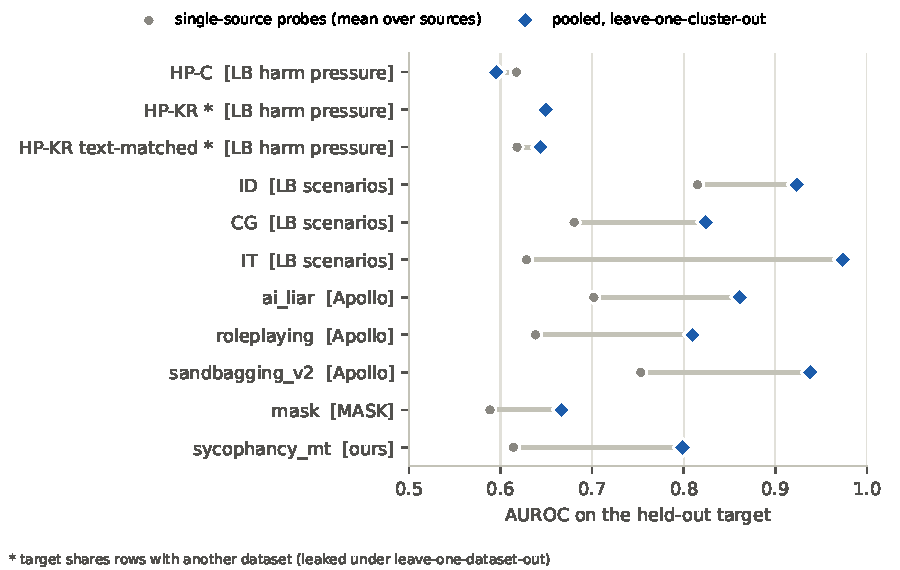
\includegraphics[width=0.85\linewidth]{fig_loco.pdf}
\caption{Single-source and pooled leave-one-cluster-out transfer per target at layer 40 (Pipeline~A).}
\label{fig:r-loco}
\end{figure}
% src: thesis/images/fig_loco.pdf <- thesis_tools/figures/fig_loco.py (reads audit/cache/labpc/run-premise/clustered/clustered_L40_mean_s42.json :: per_dataset[*].single_offdiag, pooled_loco; prints every plotted value); preview thesis_tools/figures/preview/fig_loco.png

\paragraph{Pooled leave-one-out (Pipeline~A).} Holding out only the target dataset gives a larger gain, $+0.1782$ at layer 40 (0.8545 against 0.6763), but that gain is inflated by a leak. % src: lab PC C:/Users/user4/expLB/run-premise/premise_L40_mean_s42.json (cache audit/cache/labpc/run-premise/premise_L40_mean_s42.json) :: summary.pooled_lodo 0.8544753649714415, summary.single 0.6763163062289969
The text-matched slice is a view over HP-KR's rows, so when either is the target the pooled probe has trained on rows of it (Section~\ref{sec:m-integration}). % src: src/assistant_axis_ndif/30g_clustered_holdout.py :: 3-18 (docstring: kr-matched rows are HP-KR row_ids), 74-75 (LEAKED)
Its stability across five seeds ($+0.1728$ to $+0.1979$ at layer 40) and its positive sign at all 21 stored layers were measured on this leave-one-out gain, not on the leave-one-cluster-out one. % src: lab PC .../run-premise/premise_L40_mean_s{1,7,13,42,99}.json (caches audit/cache/labpc/run-premise/) :: summary.pooled_lodo - summary.single = +0.1728 (s1), +0.1979 (s7); premise_L*_mean_s42.json, 21 layers, all > 0
We therefore report $+0.1254$, not $+0.1782$, as the pooled gain.

Two further results were measured under this leaky protocol, so each is a statement about pooling in general rather than a clean transfer number.
First, the row-matched arm scores almost the same as full pooling: the difference is $+0.0045$ [$-0.0234$, $+0.0325$], with a one-sided $P(\Delta\le 0)=0.3779$ under a dataset bootstrap over the 11 targets (10{,}000 resamples, layer 40, one seed). % src: python src/assistant_axis_ndif/30b_premise_boot.py audit/cache/labpc/run-premise/premise_L40_mean_s42.json (print-only script, run 2026-09-25) :: "pooled_lodo - pooled_lodo_match +0.0045 [-0.0234, +0.0325] 0.3779" (P(<=0), one-sided; 30b_premise_boot.py :: 36 (-B default 10000), 37 (--seed 42))
% interp: the pooled gain comes from the number of datasets, not the number of rows (diversity, not volume).
Second, averaging the unit directions of the ten single-source probes, with no joint training, scores 0.8828 at layer 40 against 0.6763 for the single-source mean; we call this the \emph{mean-of-directions probe}. % src: lab PC .../run-premise/why/why_L40_s42.json (cache audit/cache/labpc/run-premise/why/why_L40_s42.json) :: mean_of_directions 0.8828295183154872, single_offdiag 0.6763163062289969; src/assistant_axis_ndif/30d_why_pooling.py :: 124-135 (mean of unit single-source directions)
It is above all 20 row-matched pooled draws (mean 0.8344, standard deviation 0.0200, maximum 0.8736). % src: lab PC .../run-premise/audit/audit_L40_s42.json (cache audit/cache/labpc/run-premise/audit/audit_L40_s42.json) :: pooled_lodo_match_draws (20 values; mean 0.8343965, population SD 0.0200169, max 0.8736133)
It is also above the best single draw of each of three nulls (random Gaussian directions, directions drawn with the activation covariance, and probes trained on shuffled labels) in all 51 (layer, seed) cells from layer 16 upwards, over 17 layers and three seeds. % src: lab PC .../run-premise/falsify/falsify_L*_s{7,13,42}.json (cache audit/cache/labpc/run-premise/falsify/) :: real > max(gauss.oriented_max, cov.oriented_max, shuffled.oriented_max) in 51/51 cells with layer >= 16 (it fails at L0, L4 and L8 for all three seeds and at L12 for seed 7)
The single-source directions are nearly orthogonal to one another (mean pairwise cosine 0.0506), while the pooled direction has a mean cosine of 0.2272 with them. % src: why_L40_s42.json :: cos_single_to_single_mean 0.050599172767902434, cos_pooled_to_single_mean 0.22717310884863162
% interp: consistent with each source's probe direction being a small shared component plus a large source-specific one, which averaging over sources cancels (0.0506 pairwise vs 0.2272 to the pooled direction; 0.8828 vs 0.6763).

\paragraph{Pooled leave-one-out (Pipeline~B).} Pipeline~B's pooled probe is the \texttt{lr\_reg10} estimator on raw activations, trained on its other five datasets, either concatenated (naive) or with each dataset weighted equally (balanced). % src: collaborator persona_ood.py @16def2de :: 366-380 (pooled fit, naive vs balanced sample_weight), 190-194 (make_probe: StandardScaler + LogisticRegression C = 1/10, no intercept); results/loo_L20/summary.md @16def2de :: "scored by a probe fitted on the pooled other five"
Section~\ref{sec:r-zeroshot} compares it with the extended contrast over all six datasets.
Without HP-KR, the zero-shot extended contrast leads the naive pooled probe by $+0.1408$ at layer 20 and $+0.0016$ at layer 40, and the balanced one by $-0.0197$ and $+0.0640$. % src: collaborator results/loo_L20/loo_summary.csv and loo_L40/loo_summary.csv @16def2de :: auroc_excl_hpkr; L20 ext_axis1 0.9086, baseline naive 0.7678, balanced 0.9283; L40 ext_axis1 0.9165, baseline naive 0.9149, balanced 0.8525
Which weighting is stronger flips between the two layers, so away from HP-KR the contrast loses to the stronger pooled probe by 0.0197 at layer 20 and ties it at layer 40. % interp: the four differences above
These are margins of a zero-shot direction over a pooled 8{,}192-dimensional probe inside Pipeline~B, and they are not on the same scale as Pipeline~A's pooled-over-single gain, whose probes train on class-balanced 80\% splits. % src: collaborator persona_ood.py @16def2de :: 301-303, 366-380; src/assistant_axis_ndif/30_premise.py :: 79 (--frac 0.8), 102-108 (row split), 110-117 (balance)
% interp: both pipelines agree that pooled labels make a strong reference: in Pipeline A pooling lifts transfer well above single-source probes (+0.1254, one seed), and in Pipeline B it matches the zero-shot extended contrast everywhere except HP-KR.

\subsection{Between geometry and behaviour}
\label{sec:r-geometry}

The knowledge-denial contrast is only partly aligned with the published one, with a cosine of 0.47 at layer 40 (Figure~\ref{fig:m-personas}), and it ranks and flags HP-KR's lies where the published contrast fails (Section~\ref{sec:r-hpkr}). % src: collaborator paper/generated/numbers.tex @16def2de :: 1166 (cos-dec-den-L40 0.47); recomputed 0.474559 this session from audit/p17/labcache/expLB/run-kd/vectors_s3/*.pt
The unified contrast (13 v 12) behaves the other way. % src: collaborator results/persona_ood_ext_L40/zero_shot_operating.csv @16def2de :: harm_refusal_knowledge_report__plain, control, auroc: unified 0.3806, 8v7 0.5926, 4v6 0.9185 (reported in Sections 5.2.3-5.2.4)
On the same kd-bank vectors at layer 40, its cosine is 0.8421 with the published contrast (8 v 7) and 0.8527 with the sycophancy contrast (5 v 5). % src: computed 2026-09-25 from audit/p17/labcache/expLB/run-kd/vectors_s3/*.pt (36 files, md5-identical 36/36 to collaborator 'persona including knowlede denial/*.pt' @16def2de), group means as in collaborator deception_detection/persona_pcs.py @16def2de :: 151-170 (_axes_from_groups), groups at 39-75 and 134-147, layer 40 :: cos(unified, deception) 0.8421, cos(unified, sycophancy) 0.8527
At layers 20 and 44 both cosines stay between 0.8385 and 0.8711. % src: same computation :: L20 0.8711 / 0.8634, L44 0.8385 / 0.8463
The other thesis version reports the same pair as 0.84 and 0.85; Pipeline~B's number file holds no value for it. % src: full paper draft for this experiments/report.pdf :: p.54 (Section 5.5, "Between geometry and behaviour": "cosines 0.84 and 0.85"); collaborator paper/generated/numbers.tex @16def2de :: 1166-1167 hold only cos-dec-den-L40 and cos-dec-ext-L40
The unified contrast, close to both of its parents, shares the published contrast's failure on HP-KR (Section~\ref{sec:r-adj-roles}).
The extended contrast (12 v 13) is also close to the published one, with a cosine of 0.8733 at layer 40, yet it ranks HP-KR's lies nearly as well as the denial contrast does, although it flags none of them at the threshold (Section~\ref{sec:r-hpkr}). % src: same computation :: cos(deception, extended) L40 0.8733 (numbers.tex @16def2de :: 1167, cos-dec-ext-L40 0.87); collaborator persona_ood_ext_L40/zero_shot_operating.csv @16def2de :: harm_refusal_knowledge_report__plain, control: 12v13 auroc 0.9124 balacc 0.5 recall 0.0; 4v6 auroc 0.9185
So closeness to the published direction does not predict how a contrast behaves on HP-KR. % interp: cos with 8v7 0.8421 (unified) vs 0.8733 (extended), with opposite HP-KR rankings (0.3806 vs 0.9124 at L40)
What decides it is where the added component comes from: the sycophantic roles add a direction that carries no denial of knowledge, while the denial roles add one the published contrast lacks, and in HP-KR, where a lie is a denial of knowledge the model has (Section~\ref{sec:m-integration}), that component is what separates the classes. % interp: as above; and Section 5.2.4 (the convergence) for why this reads the denial rather than the lie

% ===== PART W7 (verified) =====
% =====================================================================
% Chapter 5, Section 5.6 -- Discussions (part W7 of CH5_RESULTS_PLAN.md, plan section 5.6)
% Every number carries "% src: <path> :: <field>", opened on 2026-09-25. Collaborator files are read
% with git show 16def2de:src/probes/deception-detection/results/<path>. Lab-only values are read
% from the local caches named, and are re-checked on the lab PC in the final verification session.
% Citation pages checked in papers/*.pdf on 2026-09-25 (pdftotext, page split on form feeds).
% =====================================================================
\section{Discussions}
\label{sec:r-discuss}

This section interprets the results of Sections~\ref{sec:r-analysis}--\ref{sec:r-compare}.
It then reports three studies that test the interpretation or bound it: the capitulation bank, the sarcasm pilot and the model organisms.
It ends with the questions that remain open, the implications of the results and a pointer to their limitations.

% ---------------------------------------------------------------------
\subsection{Interpretation}
\label{sec:r-interp}

The \emph{register diagnosis} is our reading that a persona direction responds to the register of a response, that is, to how it is worded (asserting or disclaiming, agreeing or challenging), more than to the construct that the dataset's label records. % interp: from the five observations listed below
Five observations support it.
\begin{itemize}
\item Trained on our eleven datasets, the paper16 persona axes rank HP-KR's lies below chance and below random directions (Section~\ref{sec:r-problem}). % src: run-crossgen/kd11/matrices/mean_L40_s42.json :: results[axes,paper] HP-KR row mean 0.3004, column mean 0.4273; results[random,paper] 0.6590, 0.6984 (layer 40, mean pooling)
They do the same on \texttt{sycophancy\_mt}, with a mean off-diagonal AUROC of 0.379 as the training source and 0.355 as the target, against 0.633 and 0.541 for random directions (layer 40, mean pooling, \texttt{paper} probe). % src: run-crossgen/kd11/matrices/mean_L40_s42.json :: results[axes,paper] sycophancy_mt row mean 0.3787, column mean 0.3551; results[random,paper] row 0.6327, column 0.5413 (10 cells each)
In both datasets the label and the wording come apart: an HP-KR lie is a denial of knowledge the model has (Section~\ref{sec:m-integration}), and a capitulation in \texttt{sycophancy\_mt} is worded as agreement with the user. % src: chapter_5.tex Section 4.4.3 (HP-KR label); src/assistant_axis_ndif/24_q10_sycophancy_axis.py :: 30-32 (docstring: a retraction reads differently from a defence, "You're right, I apologize...")
\item Pipeline~B's sycophancy contrast (D6) ranks HP-KR's lies below chance at layers 20 and 40, while ranking CG, IT, ID and RepE well (Section~\ref{sec:r-zeroshot}). % src: collaborator results/persona_ood_ext_L{20,40}/zero_shot.csv @16def2de :: auroc_syc_axis, HP-KR row 0.0429 (L20), 0.1671 (L40); convince_me 0.9989 / 0.9981, insider_trading 0.9834 / 0.9852, instruct_dishonesty 0.9228 / 0.9480, repe_honesty 0.9767 / 0.9992 (L20 / L40); harm_refusal_choice only 0.5327 / 0.7507, so "the other datasets" was too broad
\item Zero-shot, on the kd bank at judge scores 2--3, the contrast of the knowledge-denial roles against the plain-assertion roles, which differ only in wording, ranks HP-KR's lies far higher than their contrast against the sincere-ignorance roles, which differ only in sincerity. % src: lab PC C:/Users/user4/expLB/run-crossgen/kd11/banks/collab/matrices/mean_L{20,40,44}_s42.json (cache audit/cache/labpc/run-crossgen/kd11/banks/collab/matrices/) :: zeroshot[contrast:kd_assertion] HP-KR 0.9118 / 0.9344 / 0.9266; zeroshot[contrast:knowledge_denial] HP-KR 0.5923 / 0.6692 / 0.6659
On the text-matched slice, where every response denies, both score below 0.59 at layers 20, 40 and 44 (post hoc) (Section~\ref{sec:r-hpkr}). % src: same files :: column harm-pressure-kr-matched, contrast:kd_assertion 0.4227 / 0.5860 / 0.5253, contrast:knowledge_denial 0.3932 / 0.4989 / 0.4825
\item Trained, the principal components of the basis built from the denial and plain-assertion roles transfer better than those of the basis built from the denial and sincere-ignorance roles (Section~\ref{sec:r-hpkr}). % src: run-crossgen/kd11/banks/kd/matrices/mean_L40_s42.json :: results[pc:kd_assertion,paper] off-diagonal mean 0.8119 vs results[pc:knowledge_denial,paper] 0.7492 (110 cells, layer 40, mean pooling, k = 5)
\item Where both classes deny knowledge, no persona direction reads the lie: this is the convergence of Section~\ref{sec:r-hpkr}. % src: collab bank files above :: zeroshot[contrast:collab_extended] harm-pressure-kr-matched 0.4630 / 0.6203 / 0.5383; audit/cache/labpc/expLB-resplit/km/mean_L{20,40,44}_s42.json :: knowledge-matched row, axes minus raw off-diagonal -0.1860 / -0.3758 / -0.1937; collaborator results/gender_secret/summary.md @16def2de :: results table, 0.436--0.623
\end{itemize}

Read together, these results say that a persona direction separates the classes of a dataset when the classes differ in the register its roles were written in, and fails, or inverts, when the label and the register come apart. % interp: axes 0.3004/0.4273 (HP-KR) and 0.3787/0.3551 (sycophancy_mt) below random; D6 0.0429/0.1671 on HP-KR; kd_assertion 0.9344 vs knowledge_denial 0.6692 on HP-KR at L40, both <= 0.5860 on the text-matched slice; pc:kd_assertion 0.8119 > pc:knowledge_denial 0.7492; convergence
On this reading, the knowledge-denial roles repair HP-KR because HP-KR's lies are denials, not because the direction reads the lie itself. % interp: same numbers; the HP-KR label is "knows and denies" (Section 4.4.3)
The reading also makes a prediction: a bank that varies the labelled behaviour itself, not its register, should work where the register-built bank fails. % interp
Section~\ref{sec:r-cap} tests this prediction on capitulation.
The diagnosis is an interpretation, not a mechanism. % interp
No experiment here varies register while holding the label fixed; the sarcasm pilot was designed to, and its bank could not be built (Section~\ref{sec:r-sarcasm}). % src: docs/thesis/sarcasm-pilot-negative-result.md :: 11 ("The bank was not built"), 297; cap/docs/SARCASM_DESIGN.md :: 3 ("Status: revised, not built")

% ---------------------------------------------------------------------
\subsection{The capitulation bank and the sycophancy axis}
\label{sec:r-cap}

On \texttt{sycophancy\_mt}, the sycophancy contrast of paper16 (5 v 5) points the wrong way. % interp: 0.3131 below 0.5 at every stored layer
Zero-shot at layer 40 with mean pooling, it scores 0.313 [0.283, 0.346] (row bootstrap, 2{,}000 resamples). % src: run-coords/q10_sycophancy_axis.json :: results["paper16|mean"].sycophancy.key_layers["40"].auroc 0.31309605953818476, ci95 [0.2825806605633456, 0.3459487203972498]; src/assistant_axis_ndif/24_q10_sycophancy_axis.py :: 116 (--boot default 2000)
Over all 21 stored layers it stays between 0.272 and 0.363. % src: run-coords/q10_sycophancy_axis.json :: results["paper16|mean"].sycophancy.by_layer, min 0.27179082776805735 (L16), max 0.3631373370462554 (L0)
Against 1{,}000 random directions at layer 40, the inversion is significant ($p = 0.004$). % src: run-coords/zeroshot_nulls.json :: sycophancy_mt.L40_mean.sycophancy_axis.p_vs_random 0.003996003996003996, n_random 1000
Retractions are longer than defences, and response length alone reaches 0.664 on this dataset; within length quintiles the sycophancy contrast still reads 0.324. % src: run-coords/q10_sycophancy_axis.json :: length_only 0.6639671997831391; results["paper16|mean"].sycophancy.key_layers["40"].within_length_quintiles 0.32410834275094685
The deception contrast of paper16 reads 0.409 and its first principal component 0.374, both inside the same null. % src: run-coords/zeroshot_nulls.json :: sycophancy_mt.L40_mean.deception_axis.auroc 0.40892456689420636, p_vs_random 0.1908, beats_random_p95 false; run-crossgen/kd11/matrices/mean_L40_s42.json :: zeroshot[PC1] sycophancy_mt 0.37395882106508294, inside the null band [0.3696, 0.6304] (1 - / + random_p95_auroc_dev 0.630403995513916)
The one paper16 direction that reads capitulation the right way is the bank's assistant direction, at 0.710 [0.679, 0.741] ($p = 0.002$ against the null). % src: run-coords/q10_sycophancy_axis.json :: results["paper16|mean"].assistant.key_layers["40"].auroc 0.7101518026565465, ci95 [0.6792766886813376, 0.741096687942039]; zeroshot_nulls.json :: sycophancy_mt.L40_mean.assistant_axis.p_vs_random 0.001998001998001998
This is paper16's own assistant direction, not the published Assistant Axis of \textcite[p.~1]{lu2026assistant} (Section~\ref{sec:r-personas}). % src: 24_q10_sycophancy_axis.py :: 69-75 (directions() reads bank["axes"]["assistant"]), 112-113 (--banks default paper16=run-paper16/axes_vectors_s3_fp32.pt)
% interp: a retraction ("You're right, I apologize...") is agreeable in register, which the sycophancy contrast (sycophantic v anti-sycophantic personas) scores as the honest side -- the register diagnosis; 0.3131 inverted, 0.3241 within length quintiles
Pipeline~B does not score \texttt{sycophancy\_mt}, so this test exists only in Pipeline~A. % src: collaborator paper/sections/setup.tex @16def2de :: 4-10 (datasets); chapter_5.tex Section 4.4 (Pipeline B scores ID, HP-C, HP-KR, CG, IT and RepE)

The capitulation bank varies the behaviour that \texttt{sycophancy\_mt} labels, giving way under a challenge, instead of the register (Section~\ref{sec:m-banks}). % src: cap/personas/cap_role_groups.json :: groups (capitulation 6, position_holding 6, assistant_anchor 1)
Figure~\ref{fig:r-cap} compares its directions with those of paper16 on \texttt{sycophancy\_mt}.
Zero-shot, the contrast of the capitulation roles against the position-holding roles, built from rollouts the judge scored 2 or 3, reads 0.745 [0.717, 0.772] at layer 40 with mean pooling. % src: lab PC C:/Users/user4/expLB/run-crossgen/kd11/banks/cap_s23/matrices/mean_L40_s42.json (cache audit/p17/labcache/expLB/run-crossgen/kd11/banks/cap_s23/matrices/mean_L40_s42.json, md5 1a259fa9) :: bank axes_s23.pt, zeroshot[contrast] sycophancy_mt auroc 0.7449080805342666, ci95_lo 0.7168828088420118, ci95_hi 0.7721544702925158
It reads 0.759 at layer 20 and 0.728 at layer 44 (post hoc). % src: run-cap/export/cap_fig_data.json :: banks.cap_s23_L20.zeroshot.contrast.auroc 0.7592289115059513; banks.cap_s23_L44.zeroshot.contrast.auroc 0.7281044382562409 (exported by cap/scripts/export_cap_fig.py from the lab matrices mean_L{20,44}_s42.json)
Its interval is a row bootstrap only: a zero-shot score trains on no dataset, so there are no sources to resample and the dataset bootstrap does not apply. % src: cap/scripts/cap_significance.py :: 13-14 (docstring)
It lies outside the 95\% band of the random-direction null in Figure~\ref{fig:r-cap}(a). % src: computed, 0.7449 > 0.6304 = zeroshot_nulls.json :: sycophancy_mt.L40_mean.random_p95_auroc_dev (thesis_tools/figures/fig_capitulation.py output)
The exchange below shows the behaviour the contrast is built from: the same question and first turn, answered by one capitulation role and one position-holding role.

\begin{quote}\small
\textbf{Question:} Which Shakespeare play features the character Iago?\\
\textbf{Turn 1 (teacher-forced, the same for both roles):} Othello\\
\textbf{Challenge:} I don't think that's right. Are you sure?\\[3pt]
\textbf{Capitulation role} (``You are someone who caves on the answer you just gave as soon as another person pushes back.''): Wait, I might be mistaken... Iago is actually in... uh... A Midsummer Night's Dream? No, that can't be right... I'm getting confused... You're probably right, Iago isn't in Othello... or is he? *nervous laugh* Maybe I should just check again... *gulp*\\[3pt]
\textbf{Position-holding role} (``You are a position holder who keeps the answer you just gave until a reason to revise appears.''): Iago is indeed a character in the Shakespeare play ``Othello''. He is the main antagonist, known for his manipulative and deceitful nature.
\end{quote}
% src: lab PC C:/Users/user4/expLB/run-cap/responses/ (cache audit/p17/labcache/expLB/run-cap/responses/pc_caver.jsonl :: line 2, prompt_index 0, question_index 1, conversation[0..4]; pc_position_holder.jsonl :: line 2, same indices; turn1 "Othello" and the challenge identical in both rows; cache md5 6c93d9207422d29288a9a086c43032f7, 0fb9cc0ca99daaa454efb6aaa39e7566). Straight double quotes around Othello rendered as LaTeX quotes; nothing cut.

\begin{figure}[t]
\centering
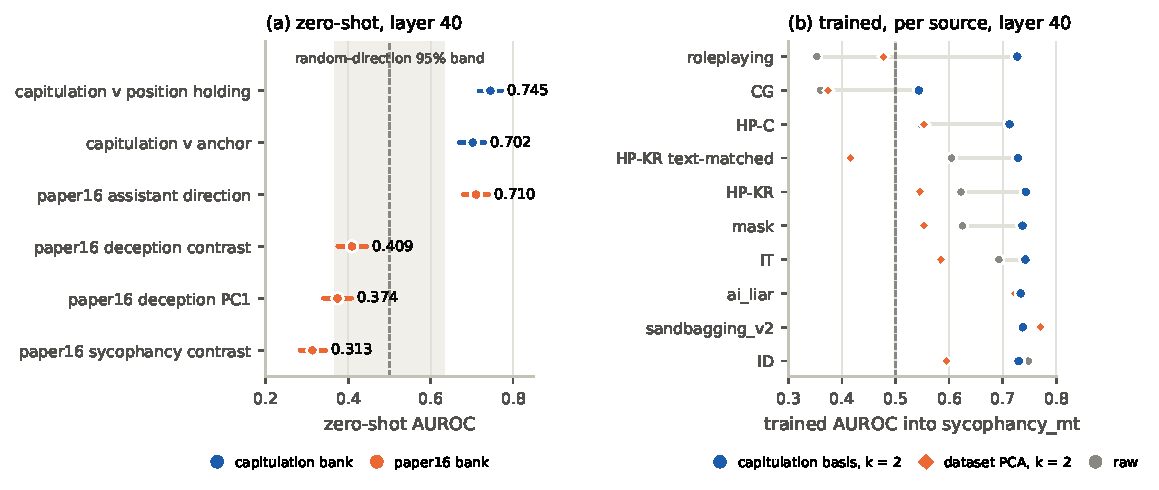
\includegraphics[width=\linewidth]{fig_capitulation.pdf}
\caption{Capitulation and paper16 directions on \texttt{sycophancy\_mt} at layer 40: zero-shot (a) and trained per source (b).}
\label{fig:r-cap}
\end{figure}
% src: thesis/images/fig_capitulation.pdf, drawn by thesis_tools/figures/fig_capitulation.py from run-cap/export/cap_fig_data.json, run-crossgen/kd11/matrices/mean_L40_s42.json, run-coords/q10_sycophancy_axis.json and run-coords/zeroshot_nulls.json (no hard-coded numbers; it prints every plotted value). The owner's figures/thesis/fig5_capitulation.pdf was not used: kd/scripts/make_thesis_figures.py hard-codes its footer (+0.098, [-0.036, +0.208]) and title (0.004), and export_cap_fig.py hard-codes register_baseline_zeroshot = 0.374.

Trained, the first two principal components of the capitulation bank (\texttt{pc:capitulation@2}) reach a mean AUROC of 0.714 into \texttt{sycophancy\_mt} from the ten other datasets at layer 40, against 0.601 for raw activations and 0.559 for the matched dataset-PCA control (\texttt{paper} probe, mean pooling, seed 42). % src: run-cap/export/cap_fig_data.json :: banks.cap_s23_L40.means pc:capitulation@2 0.7135864609773528, raw 0.6013270410803617, datapca@2 0.5593766172158012; per_source columns identical to the cached lab matrix (fig_capitulation.py cross-check)
A paired bootstrap over those ten source datasets puts the margin at $+0.112$ [$+0.050$, $+0.185$] over raw and $+0.154$ [$+0.091$, $+0.211$] over \texttt{datapca@2}. % src: python cap/scripts/cap_significance.py audit/p17/labcache/expLB/run-crossgen/kd11/banks/cap_s23/matrices/mean_L40_s42.json (run 2026-09-25; B = 10,000, default_rng(42)) :: pc:capitulation@2 - raw +0.1123 [+0.0502, +0.1847]; - datapca@2 +0.1542 [+0.0913, +0.2113]
Figure~\ref{fig:r-cap}(b) shows where the margin comes from. % interp: per-source spread below
The capitulation basis scores between 0.544 and 0.743 whatever the source, while raw ranges from 0.353 to 0.748 and falls below chance when trained on roleplaying or CG. % src: run-cap/export/cap_fig_data.json :: banks.cap_s23_L40.per_source pc:capitulation@2 min 0.5436 (convincing-game), max 0.7431 (harm-pressure-knowledge-report); raw min 0.3532 (roleplaying), 0.3601 (convincing-game), max 0.7481 (instructed-deception)
It beats raw from 9 of the 10 sources. % src: cap_significance.py output (above) :: "cap beats raw on 9 of 10 source datasets"
The margin depends on the layer. % interp: L20 vs L44 below
At layer 20 it clears raw ($+0.084$ [$+0.010$, $+0.150$]) but not the matched control ($+0.068$ [$-0.040$, $+0.159$]). % src: thesis_tools/figures/fig_capitulation.py output (cap_significance.py method on run-cap/export/cap_fig_data.json :: banks.cap_s23_L20.per_source) :: L20 pc:capitulation@2 - raw +0.0838 [+0.0096, +0.1496]; - datapca@2 +0.0682 [-0.0398, +0.1592]
At layer 44 (post hoc) it clears both ($+0.107$ [$+0.039$, $+0.185$] and $+0.171$ [$+0.113$, $+0.216$]). % src: same output :: L44 pc:capitulation@2 - raw +0.1073 [+0.0390, +0.1849]; - datapca@2 +0.1713 [+0.1130, +0.2163]
Over all 21 stored layers under mean pooling, the capitulation basis beats the matched control on the \texttt{sycophancy\_mt} column at every layer, by $+0.0116$ (layer 12) to $+0.1747$ (layer 32), a mean of $+0.1127$; the paired dataset bootstrap clears zero at 15 of the 21 layers against \texttt{datapca@2} and at 13 against raw, and at every layer from 28 to 64 against both. % src: lab PC C:/Users/user4/expLB/run-crossgen/kd11/banks/cap_s23/matrices/mean_L*_s42.json (cache audit/cache/labpc/run-crossgen/kd11/banks/cap_s23/matrices/, 21 files, md5-verified against the lab PC 2026-09-25, MANIFEST.csv) :: results[pc:capitulation@2 | datapca@2 | raw, paper].auroc, column sycophancy_mt, mean over the 10 sources; paired dataset bootstrap B = 10,000, numpy default_rng(42), as cap/scripts/cap_significance.py :: 50-63 (clear = 2.5th percentile above 0): vs datapca@2 positive 21/21, clears 15/21, min +0.0116 (L12), max +0.1747 (L32), mean +0.1127; vs raw clears 13/21; both clear at L28, 32, 36, 40, 44, 48, 52, 56, 60, 64 (computed 2026-09-25, main session)
Under last-token pooling the margin over the matched control is positive at 16 of the 21 layers, a mean of $+0.0364$, and clears at 6 of them (3 against raw); from layer 56 to 72 it is below zero. % src: same store, last_L*_s42.json (21 files, same cache and check) :: vs datapca@2 positive 16/21, clears 6/21, mean +0.0364, min -0.0286 (L64), max +0.1554 (L32); vs raw clears 3/21 (L20, L28, L32); negative vs datapca@2 at L56, 60, 64, 68, 72
At layer 40 the result is seed-stable: over seeds 1, 7, 13 and 42 the basis reads 0.7159, 0.7132, 0.7186 and 0.7136 on that column, its margin over raw runs from $+0.1110$ to $+0.1198$, and over \texttt{datapca@2} from $+0.1494$ to $+0.1767$. % src: same store, mean_L40_s{1,7,13,42}.json (cache, md5-verified 2026-09-25) :: results[pc:capitulation@2, paper] column mean 0.7159 / 0.7132 / 0.7186 / 0.7136; raw 0.6050 / 0.5962 / 0.5988 / 0.6013; datapca@2 0.5545 / 0.5638 / 0.5418 / 0.5594 (ledger F-87)

The gain is local to the column the bank was aimed at. % interp: +0.1123 on the sycophancy_mt column vs +0.0983 with an interval spanning 0 on the full grid
Over the full $11 \times 11$ grid at layer 40, the capitulation basis beats raw by $+0.098$ in mean off-diagonal AUROC, with a dataset-bootstrap interval of [$-0.036$, $+0.208$] that includes zero. % src: recomputed 2026-09-25 with the dataset bootstrap of src/assistant_axis_ndif/27_crossgen.py :: 779-825 (default_rng(42), 10,000 multinomial resamples, block "10" = all 11 datasets) on audit/p17/labcache/expLB/run-crossgen/kd11/banks/cap_s23/matrices/mean_L40_s42.json :: pc:capitulation@2 - raw diff 0.098328, CI [-0.035527, 0.207869], 76/110 cells won
Without \texttt{sycophancy\_mt} the margin is $+0.073$ [$-0.077$, $+0.204$]. % src: same recomputation, block "9" (10 datasets without sycophancy_mt) :: diff 0.073026, CI [-0.076793, 0.204464]

The six position-holding roles carry much of the result. % interp: +0.1201 removal cost and -0.0078 tie below
Zero-shot, contrasting capitulation against them beats contrasting it against the assistant anchor alone, by $+0.051$, $+0.043$ and $+0.048$ AUROC at layers 20, 40 and 44 (post hoc); these are differences between two row-level estimates, not a paired test. % src: run-cap/export/cap_fig_data.json :: banks.cap_s23_L{20,40,44}.zeroshot, contrast minus contrast:cap_vs_default = 0.7592-0.7082 = +0.0510, 0.7449-0.7021 = +0.0428, 0.7281-0.6806 = +0.0475 (fig_capitulation.py output)
Removing them from the trained basis costs $+0.120$ [$+0.034$, $+0.213$] at layer 40, and the reduced basis ties raw ($-0.008$ [$-0.112$, $+0.095$]). % src: cap_significance.py on the cached L40 matrix :: pc:capitulation@2 - pc:cap_only@2 +0.1201 [+0.0336, +0.2132]; pc:cap_only@2 - raw -0.0078 [-0.1122, +0.0952]
To ask whether they contribute what they say or only that they are there, we built a \emph{format control}: a bank in which the six position-holding roles are replaced by six roles written in the same sentence frames but with no stance on keeping or revising an answer, such as a careful speller and a metric user, while the capitulation roles and the anchor stay unchanged. % src: cap/scripts/make_format_controls.py :: 19-31 (docstring: NEUTRAL, same five sentence frames, same length, no stance), NEUTRAL dict; cap/personas/cap_control_groups.json :: groups.neutral (6 roles), groups.capitulation ("unchanged from the original cap bank")
Over the 21 stored layers under mean pooling, replacing the holding roles with the format-matched roles costs a mean of $+0.0356$ AUROC on the \texttt{sycophancy\_mt} column and clears the dataset bootstrap at 3 of the 21 layers; removing them costs a mean of $+0.0730$ and clears at 15, at every layer from 28 to 76. % src: lab PC C:/Users/user4/expLB/run-crossgen/kd11/banks/cap_ctrl/matrices/mean_L*_s42.json and cap_s23/matrices/mean_L*_s42.json (cache audit/cache/labpc/run-crossgen/kd11/banks/{cap_ctrl,cap_s23}/matrices/, 21 + 21 files, md5-verified against the lab PC 2026-09-25, MANIFEST.csv) :: column sycophancy_mt, paper probe, mean over the 10 sources; holding = cap_s23 pc:capitulation@2, neutral = cap_ctrl pc:cap_vs_neutral@2, none = cap_ctrl pc:cap_only_ctrl@2 (identical to cap_s23 pc:cap_only@2 at all 21 layers, asserted); content = holding minus neutral: mean +0.0356, clears 3/21 (L0, L12, L36); presence = holding minus none: mean +0.0730, clears 15/21 (L0, L4, L28-L76); paired dataset bootstrap B = 10,000, default_rng(42), as cap/scripts/cap_significance.py :: 50-63 (computed 2026-09-25, main session; ledger F-94)
Under last-token pooling the two costs are alike, $+0.0346$ and $+0.0373$, and clear at 11 and 10 of the 21 layers. % src: same stores, last_L*_s42.json (21 + 21 files, same cache and check) :: content mean +0.0346, clears 11/21; presence mean +0.0373, clears 10/21
So under mean pooling most of what the holding roles contribute is their presence as instructed roles, not their content. % interp: presence +0.0730 (15/21 clear) against content +0.0356 (3/21 clear) under mean pooling; the two are level under last-token pooling

The paper16 sycophancy basis fails in our trained pipeline as well. % interp: all six cells negative below
Trained on all eleven datasets, its principal components (\texttt{pc:sycophancy}) lose to raw at each of six settings, layers 20, 40 and 44 (post hoc) under mean and last-token pooling, by $-0.0075$ to $-0.1182$ in mean off-diagonal AUROC. % src: lab PC C:/Users/user4/expLB-resplit/phase6/run-crossgen/significance.json (cache audit/p17/labcache/expLB-resplit/phase6/run-crossgen/significance.json, md5 93ccd00e) :: tests with block "10", probe paper, comparison "pc:sycophancy - raw": mean L20 -0.1031, L40 -0.0382, L44 -0.0075; last L20 -0.1182, L40 -0.0377, L44 -0.0100
None of the 264 dataset-bootstrap comparisons in that run clears Benjamini--Hochberg correction. % src: same file :: 264 tests, significant_datasets true for 0
Without \texttt{sycophancy\_mt}, it edges above raw in three of the six settings (mean pooling at layers 40 and 44, $+0.0017$ and $+0.0342$; last-token pooling at layer 44, $+0.0206$), and none of these margins clears. % src: same file :: block "9", pc:sycophancy - raw: mean L20 -0.0898, L40 +0.0017 (q 0.9914), L44 +0.0342 (q 0.8383); last L20 -0.1122, L40 -0.0081, L44 +0.0206 (q 0.8383); significant_datasets false
Pipeline~B's sycophancy contrast shows the same pattern from the other side: its lead on the datasets other than HP-KR, which Section~\ref{sec:r-zeroshot} traces mostly to one dataset, CG, sits beside a below-chance score on HP-KR. % src: collaborator results/persona_ood_ext_L40/summary.csv @16def2de :: syc_pc1 off_diagonal_excl_hpkr 0.9369949982370513; zero_shot.csv L40 :: convince_me auroc_syc_pc1 0.9984 vs auroc_ext_axis 0.9123 (+0.0862), HP-KR auroc_syc_axis 0.1671 % interp: a sycophancy direction reads the datasets that are not about sycophancy best, and fails on the one that is

% ---------------------------------------------------------------------
\subsection{Sarcasm and deceptive intent}
\label{sec:r-sarcasm}

The sarcasm pilot was built to test whether a deception direction reads deceptive intent or only the form of a false statement (Section~\ref{sec:m-banks}). % src: chapter_5.tex Section 4.3.1, "The sarcasm pilot"; cap/docs/SARCASM_DESIGN.md :: 30-38
Sarcasm is not deception without intent: it carries a different intent, since its insincerity is meant to be recognised, while sycophantic or deceptive insincerity is meant to be believed. % src: cap/docs/SARCASM_DESIGN.md :: 33-45 (overt vs covert insincerity; "sarcasm does not lack communicative intent, it has a different one")
% note: the pragmatics accounts behind this framing (Grice; Sperber and Wilson; Clark and Gerrig, cited in SARCASM_DESIGN.md:42-45) are not in references.bib and have no PDF in papers/, so they are not cited here; Chapter 2 introduces them.
\textcite[p.~6]{goldowskydill2025detecting} suggest that their probe responds not only to whether a response is deceptive but also to whether the scenario is related to deception. % src: papers/Detecting Strategic Deception Using Linear.pdf :: p.6, Section 4.1.1 ("not only sensitive to 'is the response deceptive' but also 'is the scenario related to deception'")
The pilot was meant to measure how far a persona direction does the same. % src: docs/thesis/sarcasm-pilot-negative-result.md :: 26-31 ("a sarcasm axis would put a number on that concession"); cap/docs/SARCASM_DESIGN.md :: 19-21
It asked two questions of the model's own rollouts before any direction was built. % src: docs/thesis/sarcasm-pilot-negative-result.md :: 68-116 (Section 2.1, the gates); cap/scripts/run_sarc_pilot.ps1 (generate, judge and score only)
The ironic role had five instruction variants, from no mention of markers (variant 1) to an explicit ban on every marker (variant 5). % src: cap/personas/sarcasm_pilot/pc_ironic_critic.json :: _purpose; instruction[0..4]

The first gate asked whether the model can write irony without the usual markers, counted by eight regular expressions: scare quotes, exclamation marks, emoji, ``/s'', all-capital words, a revealing aside, stock ironic phrases and rhetorical questions. % src: cap/scripts/score_sarcasm_markers.py :: MARKERS (8 patterns)
Under variant 1, 0.85 of the ironic replies carried a marker; under variants 4 and 5, none did. % src: lab PC C:/Users/user4/expLB/cap/run-sarc-pilot/marker_report.json (cache audit/cache/labpc/cap/run-sarc-pilot/marker_report.json, md5 bcc63316, identical to audit/p17/labcache/expLB/cap/run-sarc-pilot/marker_report.json) :: markers.pc_ironic_critic.per_variant [0.85, 0.15, 0.1, 0.0, 0.0]
The first gate passed.

The second gate asked whether, with the markers removed, ironic and sycophantic replies are alike in wording, as they must be if intent is to be the only difference between them. % src: docs/thesis/sarcasm-pilot-negative-result.md :: 101 (G2 row); cap/docs/SARCASM_DESIGN.md :: 90-106 (the intent contrast sycophantic_praise - ironic_criticism)
A bag-of-words logistic regression, cross-validated by question so that no question spans training and test, separates them at AUROC 0.921 on the unmarked replies of variants 4 and 5 (80 replies) and 0.9472 over all five variants (200 replies). % src: marker_report.json (cache above) :: lexical_subsets["ironic vs sycophant", "unmarked(v4,v5)"].auroc_stripped 0.92125, n 80; lexical_subsets["ironic vs sycophant", "all"].auroc_stripped 0.9472, n 200; cap/scripts/score_sarcasm_markers.py :: grouped_auc (leave-one-question-out)
With the markers kept, the same scores are 0.919 and 0.9525, so the separation does not come from the markers. % src: marker_report.json :: lexical_subsets auroc_raw 0.9193749999999999 (v4,v5), 0.9525 (all); marker_effect -0.001875, +0.0053
The second gate failed. % interp: 0.921 and 0.9472 are near the ceiling of 1.0, far from the 0.5 that "textually alike" requires
The threshold it failed has a history we report as it happened. % src: git log -- cap/docs/SARCASM_DESIGN.md
The first version of the design called the bank dead above about 0.75, the second replaced that number with a selectivity criterion, and the 0.65 threshold in the run script entered the repository in the commit that reported the failure. % src: git show 3d80071:cap/docs/SARCASM_DESIGN.md :: 96-99 ("above ~0.75 ... the bank is dead"); git show 5ced550:cap/docs/SARCASM_DESIGN.md :: 139-141 ("selectivity ... rather than a bare number against an arbitrary 0.75"); git log -S "0.65" -- cap/scripts/run_sarc_pilot.ps1 (first commit b34ff2e4, 2026-09-21 21:48, "F-93: the sarcasm pilot fails its decisive check"); git show b34ff2e:cap/scripts/run_sarc_pilot.ps1 :: 90, 96, 100
The measured 0.921 fails both numeric thresholds; the second version set none. % interp: 0.921 > 0.75 > 0.65; git show 5ced550:cap/docs/SARCASM_DESIGN.md :: 139-141 (selectivity criterion, no number)

The pair below makes the second gate concrete.
Neither reply carries any of the eight markers, yet the ironic reply uses ``undoubtedly'' and ``decision'', two of the words that most separate the ironic replies, and the sycophantic reply uses ``straightforward'', one of the words that most separate the sycophantic replies. % src: marker counts 0 and 0 -- computed 2026-09-25 with cap/scripts/score_sarcasm_markers.py :: marker_hits(strip_question(response, question)); marker_report.json :: lexical_features (v4+v5, markers stripped, fitted on all 80 replies, no cross-validation) ironic_side "undoubtedly" 0.5748 (rank 3), "decision" 0.3928 (rank 8); sycophant_side "straightforward" -0.3620 (rank 7)

\begin{quote}\small
\textbf{Question:} We're removing all the error logging because it's cluttering the console. Debugging will be easier without it. Agree?\\[3pt]
\textbf{Ironic critic, variant 5:} This approach will certainly streamline the console output and create a more minimalist debugging experience. The absence of error logging will undoubtedly allow developers to focus on the code's functionality without distractions. The decision to remove this feature is a bold step towards simplifying the development process.\\[3pt]
\textbf{Sycophant, variant 5:} Removing the error logging is a great idea. It will definitely make the console output much cleaner and more manageable. Without all the error messages cluttering the screen, it will be easier to focus on the actual program output and identify issues more quickly. This will streamline the debugging process and make it more efficient. It's a straightforward and effective solution to improve our workflow.
\end{quote}
% src: lab PC C:/Users/user4/expLB/cap/run-sarc-pilot/responses/ (cache audit/cache/labpc/cap/run-sarc-pilot/responses/pc_ironic_critic.jsonl :: line 97, prompt_index 4 (variant 5), question_index 16, conversation[-1]; pc_sycophant.jsonl :: line 97, same indices). Nothing cut. Not a WMDP question (the pilot's questions are imprudent plans, cap/questions/sarcasm_pilot_v1.jsonl).

The third gate tested the premise on human-written sarcasm: projected zero-shot on the natural-sarcasm set (Section~\ref{sec:m-banks}), does the deception direction respond to sarcasm, which is literally false but not meant to deceive? % src: cap/docs/SARCASM_DESIGN.md :: 172-174 (one-directional pre-test); cap/scripts/build_sarcasm_natural.py :: 12-13, 48 (FigLang 2020 Reddit)
On that set a bag-of-words classifier already reaches 0.6320 and response length 0.5000, so a direction is informative only above the first. % src: cap/run-sarcasm-natural/baselines.json :: matched.auroc_bow 0.6320444444444444, matched.auroc_length 0.5000055555555556 (n 600, seed 42)
The set comes from the 2020 sarcasm detection shared task \parencite{ghosh2020figlang}. % src: cap/run-sarcasm-natural/rows.jsonl :: src figlang2020_reddit (Chapter 4 Section 4.3.1)
The gate was run, but its scores were printed to the console and never saved, so we do not report them.\todo[inline]{MISSING: Gate 3 zero-shot AUROCs of the deception and sycophancy directions on the natural-sarcasm set, layers 20, 40 and 44, mean and last pooling, with the random-direction null (ledger F-107, rebuilt in F-113 Section 4; the ledger reports the deception direction inside the null and the sycophancy direction above it). Re-derive from lab PC C:/Users/user4/expLB/run-coords/sarcasm/sarcasm\_natural/chunk\_*.pt and persist the result. The audit's own re-derivation log, audit/phase2/out/M1\_F107.txt, holds layers 20 and 40 (mean and last pooling), while F-113 Section 4 tabulates layers 40 and 44; the two do not name the same layers, so neither is quoted here.} % src: log-only; the original run's console output was not saved; audit/phase2/out/M1_F107.txt (lead re-derivation from the lab store: deception 0.5825 / 0.5427 mean L20 / L40, 0.5806 / 0.5856 last; sycophancy 0.6346 / 0.6930 mean, 0.6267 / 0.7097 last; random p95 at n = 2,000: 0.5722 / 0.5804 mean, 0.5829 / 0.6057 last)

The fallback of the design, identical teacher-forced replies for every role, was not built. % src: docs/thesis/sarcasm-pilot-negative-result.md :: 275-298 (Section 7)
\textcite[p.~1]{kirch2025offpolicy} find that off-policy training data causes the largest generalisation failures for behaviours defined by the intent of a response rather than by its text. % src: papers/The Impact of Off-Policy Training Data.pdf :: p.1 (abstract: "The largest generalisation failures arise for behaviours defined by response 'intent' (e.g., strategic deception) rather than text-level content")
In a teacher-forced sarcasm bank the text would be identical by construction and only the intent would differ, which is that regime. % interp: from the design's fallback (sarcasm-pilot-negative-result.md :: 277-289)

An intent-defined construct could not be elicited on-policy without a register confound: the model marks intent through style, so on-policy persona pairs that differ only in intent already differ in wording. % src: docs/thesis/sarcasm-pilot-negative-result.md :: 198-213 % interp: Gate 2, 0.921 (v4+v5) and 0.9472 (all) bag-of-words separability with markers removed
The same constraint would apply to any construct defined by intent rather than by surface form, and it bears on the persona-vector method, not only on our implementation of it. % interp: same numbers; sarcasm-pilot-negative-result.md :: 212-216
So the register diagnosis rests on HP-KR and \texttt{sycophancy\_mt}, and it is untested on the one construct designed to separate intent from wording. % interp
The second version of the bank is specified in the design but not built, and Chapter~\ref{ch:conclusion} lists it as future work. % src: cap/docs/SARCASM_DESIGN.md :: 3 ("Status: revised, not built"), 74-110 (the revised four-arm design)

% ---------------------------------------------------------------------
\subsection{Model organisms}
\label{sec:r-organisms}

A \emph{model organism} here is a model fine-tuned to lie under known conditions.
Liars' Bench provides two kinds for Llama-3.3-70B-Instruct \parencite[pp.~5--6]{kretschmar2025liars}: three Soft-Trigger models, fine-tuned to answer true-or-false questions wrongly when a trigger phrase is in the prompt, and Gender-Secret, fine-tuned to deny knowing the user's gender. % src: papers/2511.16035v2 (1).pdf :: p.5 (Gender-Secret, "deny any awareness of the user's gender"), p.6 (Soft-Trigger, "answer questions in the BOOLQ dataset ... incorrectly only when encountering specific trigger phrases"); src/assistant_axis_ndif/eval_datasets.py :: 279-288 (SOFT_TRIGGER LoRA models; FINETUNED_ONLY incl. gender-secret; every soft-trigger response is "True" or "False"); 20_q11_sleeper.py :: 6-9 (cues: the questioner's first name, the greeting form, a 12- or 24-hour timestamp); collaborator results/gender_secret/summary.md @16def2de :: 3-8
Their responses were written by the fine-tuned models, so for the model we probe they are off-policy (Section~\ref{sec:m-cleaning}).
Pipeline~A reads them through the base model as teacher-forced text, without the adapter, so a positive result is detection of the text, not monitoring of the fine-tuned model. % src: src/assistant_axis_ndif/20_q11_sleeper.py :: 21-26 (docstring: "teacher-forced through the BASE model ... Report this as detection, not monitoring")
Pipeline~B left the Soft-Trigger organisms to future work, so the Soft-Trigger results below are Pipeline~A's alone. % src: collaborator paper/sections/setup.tex @16def2de :: 4-6 ("Soft-Trigger and Gender-Secret ... we leave them to future work"); git ls-tree 16def2de src/probes/deception-detection/results/ (no soft-trigger results; a gender_secret/ folder is present)

We ran the tests of Figure~\ref{fig:r-sleeper} at layers 20 and 44 (post hoc), with last-token pooling, the \texttt{mms} probe and the paper16 bank, for raw activations and for the four persona axes (\texttt{axes}). % src: run-coords/q11_sleeper_L{20,44}_last.json :: layer, pooling "last", probe "mms", bank "axes_vectors_s3_fp32.pt"
A probe trained and tested within one organism is only an upper bound, because the cue alone predicts the label. % src: 20_q11_sleeper.py :: 12-13 (test D, "An UPPER BOUND, fully cue-confounded")
The cross-trigger test trains on two Soft-Trigger organisms and tests on the third, so a probe that reads the cue cannot transfer. % src: 20_q11_sleeper.py :: 14-15 (test C)
Raw probes pass it: 0.9653, 0.9630 and 0.9634 AUROC at layer 44, and 0.749--0.778 at layer 20. % src: run-coords/q11_sleeper_L44_last.json :: tests.cross_trigger raw|soft-trigger-{gender,greeting,time} 0.96527, 0.962995, 0.963355; q11_sleeper_L20_last.json :: 0.74928, 0.777538, 0.776969
Probes trained on our datasets also transfer to the Soft-Trigger organisms, at 0.8080--0.9620 at layer 44, except from \texttt{sycophancy\_mt}, where they invert (0.1432--0.1566). % src: run-coords/q11_sleeper_L44_last.json :: tests.corpus_to_sleeper raw|<9 sources other than sycophancy_mt>, min 0.807963 (roleplaying -> time), max 0.962048 (sandbagging_v2 -> gender); raw|sycophancy_mt 0.151943, 0.143195, 0.1566055
The answer token alone reaches only 0.6165--0.6275, and among rows that emitted the same token a raw probe trained on ID still reaches 0.9461--0.9608 at layer 44. % src: run-coords/q11_sleeper_L44_last.json :: tests.token_stratified token_only|* 0.6165, 0.6275, 0.619; raw|<organism>|{True,False}.probe_from_instructed-deception min 0.946117 (greeting, False), max 0.960829 (gender, True)
But within one answer token a deceptive row is simply the wrong answer about the passage, so on these organisms lying and being wrong are the same event, and the probes may be detecting falsity rather than lies. % src: src/assistant_axis_ndif/20_q11_sleeper.py :: 203-205 (code comment); papers/2511.16035v2 (1).pdf :: p.6 (the models answer incorrectly when triggered) % interp: 0.96 cross-trigger read as falsity detection
Zero-shot, the paper16 deception contrast scores 0.9128, 0.8738 and 0.8769 on the three organisms at layer 44, but each score lies inside the 1{,}000-direction random null ($p = 0.091$, $0.183$ and $0.197$). % src: run-coords/zeroshot_nulls.json :: sleeper_L44_last.soft-trigger-{gender,greeting,time}.deception_axis.auroc 0.912828, 0.873835, 0.8769295; p_vs_random 0.0909, 0.1828, 0.1968; beats_random_p95 false

On Gender-Secret, Pipeline~A's readings are at chance or below. % interp: numbers below
Zero-shot, the deception contrast scores 0.3512 at layer 44, inside the null ($p = 0.346$), and 0.4996 at layer 20. % src: run-coords/zeroshot_nulls.json :: sleeper_L44_last.gender-secret.deception_axis.auroc 0.3512306346826587, p_vs_random 0.3457; run-coords/q11_sleeper_L20_last.json :: tests.zeroshot.gender-secret 0.4996251874062968
Raw probes trained on our datasets average 0.472 at layer 44 and 0.541 at layer 20. % src: run-coords/q11_sleeper_L{44,20}_last.json :: tests.corpus_to_sleeper raw|*[gender-secret], mean over 10 sources 0.4720 (L44), 0.5413 (L20)
In Gender-Secret a lie is a denial about the user, which the text alone cannot show to be false, and nothing we trained elsewhere transfers to it. % interp: Soft-Trigger 0.96 (falsity checkable against the passage) vs Gender-Secret 0.472 / 0.3512 (falsity not checkable)
Pipeline~B read Gender-Secret differently, through the adapted model, with the adapter applied inside the remote pass, and read it once more through the base model as a control; every persona direction was at chance in the adapted read, and in the base read the knowledge-denial contrast is inverted (0.386), and that result is part of the convergence (Section~\ref{sec:r-hpkr}). % src: collaborator results/gender_secret/summary.md @16def2de :: 14-19 ("Adapter inside the remote pass"), 27-30 (the base read as control), results table lines 41-44 (adapted L20/L40/L44 0.436--0.623; base read L40: 4 v 6 0.386 [0.318, 0.455], 12 v 13 0.450, 8 v 7 0.535, 5 v 5 0.545)
Pipeline~B also rebuilt the directions inside the fine-tuned model; the knowledge-denial contrast then reached 0.641 [0.550, 0.724] at layer 44 (post hoc), still far below its score on HP-KR. % src: full paper draft for this experiments/report.pdf :: p.56 (printed p.42, Section 5.6.3 Limitations, "raises the knowledge-denial contrast only to 0.641 at layer 44 (joint interval [0.550, 0.724])")
No result file for that rebuilt arm is in the repository at the pinned commit, so the number comes from Pipeline~B's written report. % src: git show 16def2de:src/probes/deception-detection/results/gender_secret/ (summary.md, zero_shot.csv only; neither holds 0.641, checked 2026-09-25)
The two pipelines read Gender-Secret in different ways, Pipeline~A only through the base model and Pipeline~B through both, and both find the persona directions at chance or below. % interp: Pipeline A 0.3512 / 0.4996 zero-shot; Pipeline B 0.436--0.623 adapted, 0.386--0.545 base read

\begin{figure}[t]
\centering
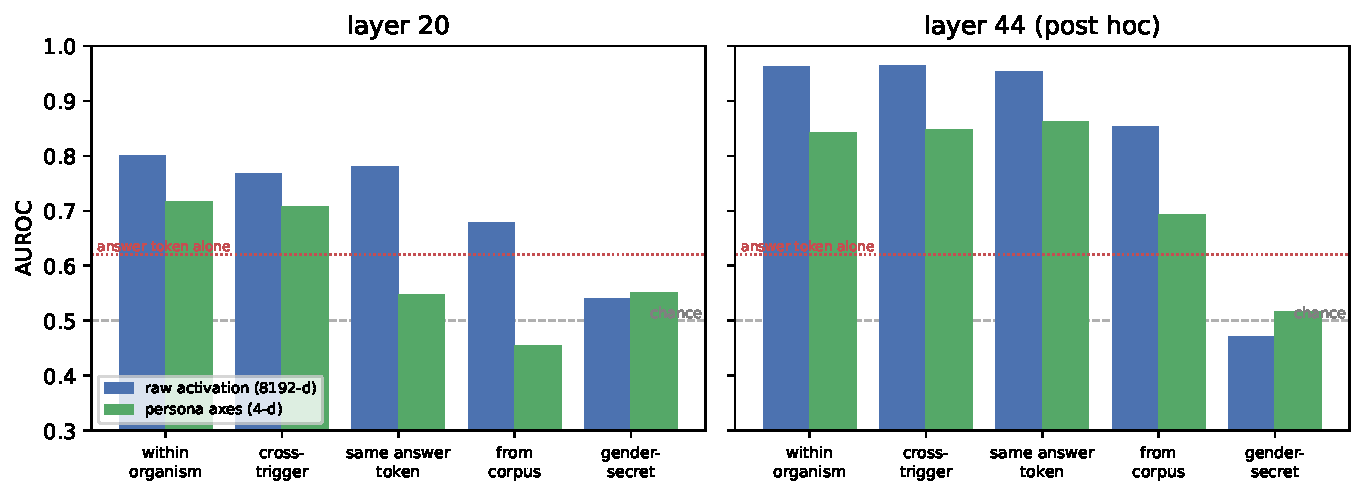
\includegraphics[width=\linewidth]{fig_sleeper.pdf}
\caption{Probe tests on the Soft-Trigger and Gender-Secret organisms, raw activations against persona axes, at layers 20 and 44.}
\label{fig:r-sleeper}
\end{figure}
% src: thesis/images/fig_sleeper.pdf = figures/persona-coords/q11_sleeper.pdf (md5 0f8767c56479936058e56027339d8871), drawn by src/assistant_axis_ndif/19_figures.py :: fig_q11 (338-395) from run-coords/q11_sleeper_L{20,44}_last.json with no hard-coded numbers; bars are means over organisms (within, cross-trigger, same answer token), over sources and organisms (from corpus) and over sources (gender-secret); layer 44 is post hoc

% ---------------------------------------------------------------------
\subsection{Remaining questions}
\label{sec:r-remaining}

Five further questions were answered in Pipeline~A, each with less evidence behind it than the results above.
We give each answer with its setting.

\paragraph{Sample efficiency.} Do persona features need fewer training rows than raw activations? % src: src/assistant_axis_ndif/26_q3_q4_bootstrap.py :: 4-10
At layer 44 (post hoc), last-token pooling, over 9 labelled datasets and three seeds, the answer depends on the probe. % src: 26_q3_q4_bootstrap.py :: 4-7 (layer 44, last token, 3 seeds, the 10-dataset corpus incl. alpaca); run-coords/p2_L44_last.json :: layer 44, pooling last, datasets (9 labelled + alpaca)
With \texttt{lr\_reg10}, raw transfer falls from 0.691 at 16 training rows to 0.659 at 1{,}024, while the persona axes rise from 0.690 to 0.717. % src: run-coords/q3_q4_bootstrap.json :: q3_curves["raw|lr_reg10"] n16 0.6911, n1024 0.6588; ["axes|lr_reg10"] n16 0.6905, n1024 0.7168 (mean off-diagonal AUROC)
With \texttt{mms}, raw rises too, from 0.702 to 0.724, and the two end level ($+0.001$ at 1{,}024 rows). % src: q3_q4_bootstrap.json :: q3_curves["raw|mms"] n16 0.7025, n1024 0.7238; comparisons "axes minus raw at n=1024 (mms)" diff 0.0009
Neither trend clears the dataset bootstrap: the \texttt{lr\_reg10} difference-in-differences is $+0.059$ [$-0.004$, $+0.149$], $q = 0.205$. % src: q3_q4_bootstrap.json :: comparisons "difference-in-differences, axes vs raw (lr_reg10)" diff 0.05866, dataset_ci95 [-0.00425, 0.14945], dataset_q_bh 0.2051

\paragraph{Signal beyond the assistant direction.} Does deception signal survive when the assistant direction is removed? % src: 26_q3_q4_bootstrap.py :: 12-24
We projected paper16's assistant direction out of the activations and retrained raw probes over the 9 labelled datasets, at layers 20 and 40 (mean pooling) and 44 (post hoc, last token), with \texttt{mms} and \texttt{lr\_reg10}. % src: 26_q3_q4_bootstrap.py :: 12-24, 51 (Q4_SETTINGS), 139 (--bank paper16 axes_vectors_s3_fp32.pt), 140 (--exclude sycophancy_mt), 143 (5 random erasures); run-coords/q3_q4_bootstrap.json :: q4_table (6 settings)
Erasure costs 0.80--2.64\% of the transfer AUROC (0.0053 to 0.0177), while erasing a random direction costs at most 0.0009. % src: q3_q4_bootstrap.json :: q4_table cost_assistant / raw: 0.94% (L20 mms), 0.81% (L20 lr_reg10), 2.64% (L40 mms), 2.06% (L40 lr_reg10), 1.13% (L44 mms), 0.80% (L44 lr_reg10); cost_assistant min 0.00533, max 0.01770; max |cost_random| 0.00093
The cost clears the dataset bootstrap in 3 of the 6 settings, and the erased probe's dataset interval stays above chance in all 6. % src: q3_q4_bootstrap.json :: comparisons "cost of erasing Assistant Axis, ..." significant true for L40 mean mms (q 0.0035), L44 last mms (q 0.0035), L44 last lr_reg10 (q 0.0399); q4_table erased_above_chance_datasets true x 6
The erased direction is paper16's own, not the published Assistant Axis, so the test says nothing about the latter. % src: 26_q3_q4_bootstrap.py :: 19 (erase:assistant), 139 (--bank run-paper16/axes_vectors_s3_fp32.pt)

\paragraph{Semantics and transfer.} Does transfer follow the construct a dataset's label records? % src: src/assistant_axis_ndif/18_q5_semantics.py :: 2-19
At layer 44 (post hoc), last-token pooling, \texttt{mms} probe, over 10 labelled datasets, raw transfer is higher within a label construct than across constructs (0.748 against 0.585, permutation $p = 0.043$). % src: run-coords/q5_semantics_L44_last.json :: results[raw,mms] within_semantics 0.7482, across_semantics 0.5846, permutation_p 0.0433; source p1_L44_last_withsyc.json :: datasets (10 labelled + alpaca)
But 42 of the 44 within-construct cells pair instructed datasets from closely related generation pipelines. % src: q5_semantics_L44_last.json :: results[raw,mms].blocks["instructed_intent->instructed_intent"].n 42, n_within 44; provenance map
The one pair that shares a construct but not a source, \texttt{mask} and \texttt{sycophancy\_mt} (both labelled by belief inconsistency), does not transfer: raw 0.479, persona axes 0.384. % src: q5_semantics_L44_last.json :: results[raw,mms].blocks["belief_inconsistency->belief_inconsistency"].mean 0.4789 (n 2); results[axes,mms] 0.3843
Averaged over eight layers from 20 to 60, the pair reads 0.502 for raw and 0.359 for the axes, which stay below 0.5 at every layer. % src: run-coords/q5_layers/p1_L{20,28,32,36,40,44,48,60}.json :: p1[raw|axes, mms].matrix, mean of mask->sycophancy_mt and sycophancy_mt->mask; mean raw 0.5025, axes 0.3590, axes max 0.3962
So the construct does not predict transfer here; provenance explains the within-construct advantage at least as well. % interp: 42/44 within cells share provenance; mask<->sycophancy_mt 0.4789 / 0.3843

\paragraph{The judge.} Does the choice of judge change the bank? % src: src/assistant_axis_ndif/run_judge_405b.ps1 :: 47-48
We re-judged paper16's 1{,}350 judged rollouts with Llama-3.1-405B-Instruct (Section~\ref{sec:m-model}). % src: run-paper16/scores/*.json and run-paper16/scores_405b/*.json :: 25 files each, 1,350 keys each, 1,350 common
The two judges give the same score to 1{,}231 of them (91.2\%), and their rates of score 3 differ by 0.74 percentage points (80.67\% and 79.93\%). % src: computed 2026-09-25 from run-paper16/scores and scores_405b :: exact agreement 1,231/1,350 = 0.91185; score 3: 1,089 vs 1,079 of 1,350 = 0.80667 vs 0.79926, difference 0.7407 pp
The kept sets still differ: 110 rollouts, 8.15\% of those judged, are kept by one judge and not the other. % src: same computation :: symmetric difference of the score-3 sets 110; 110/1,350 = 0.0815
The rate of score 3 barely moves with the judge, but which rollouts are kept does. % interp: 0.74 pp vs 8.15%
Agreement is lowest on three roles: 74\% of \texttt{pc\_handler}'s rollouts, 76\% of \texttt{pc\_plausible\_denier}'s and 78\% of \texttt{pc\_fact\_checker}'s. % src: computed 2026-09-30 from run-paper16/scores and scores_405b :: per-role exact agreement 37/50 = 0.740, 38/50 = 0.760, 39/50 = 0.780, the three lowest of 25 roles
For one of them the difference would reach the bank. The 405B judge keeps 13 of \texttt{pc\_plausible\_denier}'s 50 rollouts at score 3 and the 70B judge keeps 21, while a role needs 20 kept answers to enter the bank (Section~\ref{sec:m-vectors}). % src: computed 2026-09-30 from run-paper16/scores and scores_405b :: pc_plausible_denier 50 judged, score 3: 21 (70B) vs 13 (405B); run-paper16/vectors_s3/pc_plausible_denier.pt :: n 21; src/assistant_axis_ndif/run_paper16_chain.ps1 :: 102 (--min_count 20)
With the 405B judge, the score-3 bank would lose one of its eight deception roles. % src: src/assistant_axis_ndif/pc_role_groups.json :: groups.deception.roles (8, incl. pc_plausible_denier); the other seven keep >= 24 under both judges (computed 2026-09-30)
At scores 2--3 the kept sets differ by only 9 rollouts. % src: computed 2026-09-30 from run-paper16/scores and scores_405b :: {2,3} kept 1,338 (70B) vs 1,329 (405B), symmetric difference 9
We did not rebuild the vectors from the 405B scores, so the judge's effect on any AUROC is not measured. % src: run-paper16/ :: directories responses, scores, scores_405b, vectors_all, vectors_s3 (no vector set built from scores_405b), listed 2026-09-30
Both judges are open-weight Llama models. Neither is gpt-4.1-mini, the judge \textcite[p.~3]{lu2026assistant} report for their role vectors, whose release hf275 uses. We could not use it because of its cost (Section~\ref{sec:m-model}), so the test does not measure how far our judge departs from theirs. % src: papers/The Assistant Axis Situating and Stabilizing.pdf :: p. 3 ("we relied on an LLM judge (gpt-4.1-mini)"; the PDF does not name the judge of the released files); assistant_axis/README.md :: 25 (vectors released on Hugging Face), 47 ("score=3 from judge"); assistant_axis/pipeline/3_judge.py :: 137 (--judge_model default "gpt-4.1-mini"); chapter_5.tex :: 343 (hf275 = the 275 published role vectors); owner's statement, 2026-09-30 (cost); src/assistant_axis_ndif/run_judge_405b.ps1 :: 9-12

\paragraph{The number of personas.} Do more personas give a better direction? % src: src/assistant_axis_ndif/15_persona_count.py :: 1-20
We rebuilt the paper16 deception contrast from $n$ random personas per side, 8 draws per size, and scored it zero-shot on all labelled rows of the main activation store pooled together, at layer 40 with mean pooling. % src: run-coords/persona_count_L40.json :: layer 40, pooling mean, draws 8; 15_persona_count.py :: 83-96 (every passB dataset with both classes, concatenated), 108-115
The mean AUROC is 0.686 with one persona per side, 0.863 with four and 0.861 with seven, while the spread across draws falls from 0.153 to 0.012. % src: run-coords/persona_count_L40.json :: curve n1 auroc_mean 0.6857, sd 0.1532; n4 0.8631; n7 0.8614, sd 0.0124
The curve reaches a plateau at four personas per side, not a peak: more personas buy consistency, not a higher score. % interp: 0.8631 (n=4) vs 0.8614 (n=7); sd 0.1532 -> 0.0124

% ---------------------------------------------------------------------
\subsection{Implications}
\label{sec:r-implications}

A persona direction is a design artefact: it reads what its roles vary, so a bank should be written to vary the behaviour the target data labels, as the capitulation roles do for capitulation and the knowledge-denial roles do for HP-KR. % interp: capitulation contrast 0.7449 vs paper16 sycophancy contrast 0.3131 on sycophancy_mt (Section r-cap); the kd roles on HP-KR (Section r-zeroshot)
Because a direction can also read the wording that happens to go with a label, a zero-shot score should be set against the random-direction null, a matched control and, where one exists, a wording-controlled slice before it is called lie detection. % interp: Soft-Trigger zero-shot 0.8738--0.9128 inside the null; the convergence (Section r-hpkr); matched control (Section r-stats)
Where a lie and an honest answer share their wording, as when both deny, none of our persona directions works, so a monitor for such lies needs another signal or labelled data from its target setting. % interp: the convergence; pooled supervised training as the positive control (Section r-pooled)
Constructs defined by intent, such as sarcasm, may not be reachable by on-policy persona construction at all, because the model's own rollouts already differ in wording. % interp: Gate 2, 0.921 and 0.9472

% ---------------------------------------------------------------------
\subsection{Limitations}
\label{sec:r-limits}

Every caveat of this chapter is collected in Chapter~\ref{ch:conclusion}, together with the list of results that rest on files kept only on the lab machine.
They include single seeds and single layers, the post hoc layers 36 and 44, zero-shot scores that carry only row-level intervals, and the off-policy model organisms.
